\documentclass[aspectratio=169, 10pt]{beamer}
\useinnertheme{rounded}
\useoutertheme{infolines}
\usecolortheme{whale}
\usecolortheme{orchid}
\usefonttheme{serif}

% Package for non-counting appendix slide numbers
\usepackage{appendixnumberbeamer}

% Standard Packages
\usepackage[utf8]{inputenc}
\usepackage[T1]{fontenc}
\usepackage[english]{babel}
\usepackage{graphicx}
\usepackage{booktabs}
\usepackage{amsmath, amssymb, amsthm}
\usepackage{hyperref}
\usepackage{xcolor}
\usepackage{subcaption} 
\usepackage{bbm} 
\usepackage{array}
\usepackage{tabularx}
\usepackage{multirow}
\usepackage[most]{tcolorbox}
\usepackage{tikz}

% Custom Color Palette
\definecolor{forestgreen}{RGB}{46, 90, 60}
\definecolor{lightleaf}{RGB}{240, 245, 238}
\definecolor{moss}{RGB}{138, 154, 91}
\definecolor{darkforest}{RGB}{30, 65, 42}
\definecolor{alertred}{RGB}{180, 50, 40}
\definecolor{terracotta}{RGB}{209, 107, 89}
\definecolor{mutedgold}{RGB}{217, 178, 76}
\definecolor{emerald}{RGB}{35, 130, 75}
\definecolor{lightemerald}{RGB}{90, 215, 170}
\definecolor{cobaltblue}{RGB}{64, 133, 184}



% Beamer Theme Color Customizations
\setbeamercolor{frametitle}{bg=lightleaf, fg=forestgreen}
\setbeamercolor{headline}{bg=forestgreen, fg=white}
\setbeamercolor{footline}{bg=lightleaf, fg=forestgreen}
\setbeamercolor{structure}{fg=forestgreen}
\setbeamercolor{normal text}{fg=black, bg=white}
\setbeamercolor{block title}{bg=forestgreen!15, fg=forestgreen!70!black}
\setbeamercolor{block body}{bg=white}

% Suppress navigation symbols and configure clean 16:9 headline/footline
\setbeamertemplate{navigation symbols}{}
\setbeamertemplate{headline}{%
  \leavevmode%
  \hbox{%
  \begin{beamercolorbox}[wd=.5\paperwidth,ht=2.5ex,dp=1.1ex,right]{section in head/foot}%
    \usebeamerfont{section in head/foot}\textbf{\insertsectionhead}\hspace*{2ex}
  \end{beamercolorbox}%
  \begin{beamercolorbox}[wd=.5\paperwidth,ht=2.5ex,dp=1.1ex,left]{subsection in head/foot}%
    \usebeamerfont{subsection in head/foot}\hspace*{2ex}\insertsubsectionhead
  \end{beamercolorbox}}%
  \vskip0pt%
}

% Custom tcolorbox Environments with tight padding to prevent overfull vbox
\tcbset{
  leafbox/.style={
    enhanced,
    colback=lightleaf!80!white,
    colframe=forestgreen!60!black,
    coltitle=forestgreen!70!black,
    fonttitle=\bfseries,
    boxrule=0.5pt,
    frame hidden,
    borderline west={3pt}{0pt}{forestgreen!70!black},
    sharp corners,
    colbacktitle=forestgreen!10!white,
    top=2pt, bottom=2pt, left=4pt, right=4pt,
    toptitle=1pt, bottomtitle=1pt
  },
  takeawaybox/.style={
    enhanced,
    colback=lightleaf!40!white,
    colframe=forestgreen,
    coltitle=forestgreen!80!black,
    fonttitle=\bfseries\small,
    boxrule=0.5pt,
    borderline west={3.5pt}{0pt}{forestgreen},
    sharp corners,
    colbacktitle=lightleaf,
    top=2pt, bottom=2pt, left=4pt, right=4pt,
    toptitle=1pt, bottomtitle=1pt
  },
  alertleafbox/.style={
    enhanced,
    colback=red!5!white,
    colframe=alertred!80!black,
    coltitle=alertred!90!black,
    fonttitle=\bfseries\small,
    boxrule=0.5pt,
    borderline west={3.5pt}{0pt}{alertred},
    sharp corners,
    colbacktitle=red!10!white,
    top=2pt, bottom=2pt, left=4pt, right=4pt,
    toptitle=1pt, bottomtitle=1pt
  }
}

\newcommand{\ind}[1]{\mathbbm{1}_{\{#1\}}}

% Presentation Metadata
\title[Should I Save \textit{and} Should I Go?]{\textbf{Should I Save \textit{and} Should I Go?}}
\subtitle{A Spatial Model of Climate Change Adaptation with Saving and Migration}
\author[L. Chapuis]{\textbf{Léon Chapuis}}
\institute[PSE / ENS--PSL]{Paris School of Economics / École normale supérieure--PSL}
\date[Summer 2026]{Master APE Thesis Defense --- Summer 2026}

\begin{document}

% =========================================================================
% TITLE SLIDE (Uncounted)
% =========================================================================
\begin{frame}[plain, noframenumbering]
  \titlepage
\end{frame}

% =========================================================================
% SECTION 1: INTRODUCTION (SLIDES 1 TO 5)
% =========================================================================
\section{Introduction}

% SLIDE 1: OUTLINE
\begin{frame}{Presentation Outline}\label{main:outline}
    \begin{enumerate}\setlength{\itemsep}{6pt}
        \item[\textbf{I.}] \textbf{Motivation \& Research Question} 
        \item[\textbf{II.}] \textbf{The Dynamic Spatial Framework}
        \item[\textbf{III.}] \textbf{Saving Motives \& Calibration} 
        \item[\textbf{IV.}] \textbf{Quantitative Results \& Counterfactuals}
        \item[\textbf{V.}] \textbf{Conclusion \& Limitations} 
    \end{enumerate}
\end{frame}

% SLIDE 2: FACT #1 — CLIMATE CHANGE IS UNDERWAY
\begin{frame}{Fact \#1: Climate Change is Underway \hfill \hyperlink{backup:climate_facts}{\scriptsize\beamergotobutton{IPCC Details}}}\label{main:fact1}
    \begin{itemize}\small
        \item \textbf{Global Warming Trajectory:}
        \begin{itemize}\footnotesize
            \item Global mean surface temperature is already $+1.1^\circ\text{C}$ above pre-industrial baseline.
            \item IPCC AR6 projects $+2.0^\circ\text{C}$ to $+4.0^\circ\text{C}$ warming by 2100 under SSP5-8.5 (IPCC, 2023).
        \end{itemize}
        \vspace{0.06cm}
        \item \textbf{Mitigation Policies Repeatedly Fall Short:}
        \begin{itemize}\footnotesize
            \item Paris Agreement commitments face an emissions gap of $15\text{--}20\text{ GtCO}_2\text{e}$ by 2030 (Barrage \& Nordhaus, 2023).
        \end{itemize}
        \vspace{0.06cm}
        \item \textbf{Surging Frequency of Extreme Climatic Events:}
        \begin{itemize}\footnotesize
            \item 1-in-50 year extreme heat events occur $4.8\times$ more frequently; Western US wildfire burn area up $>400\%$ since 1984.
        \end{itemize}
    \end{itemize}
    \vspace{0.1cm}
    \begin{tcolorbox}[takeawaybox, title=Economic Implication]
        \footnotesize Households cannot rely solely on international mitigation; \textbf{individual adaptation} and behavioral adjustments (saving and migration) have become first-order economic necessities.
    \end{tcolorbox}
\end{frame}

% SLIDE 3: FACT #2 — SPATIALLY HETEROGENEOUS IMPACT
\begin{frame}{Fact \#2: Climate Change is Spatially Heterogeneous \hfill \hyperlink{backup:hsiang_method}{\scriptsize\beamergotobutton{Hsiang Method}}}\label{main:fact2}
    \begin{columns}[T]
        \begin{column}{0.48\textwidth}
            \begin{itemize}\footnotesize
                \item \textbf{Extreme Spatial Disparity:}
                \begin{itemize}\scriptsize
                    \item Climate damages do not affect all regions equally (Burke et al., 2015; Hsiang et al., 2017).
                \end{itemize}
                \vspace{0.04cm}
                \item \textbf{Severe Losses in the US South:}
                \begin{itemize}\scriptsize
                    \item Southern and Gulf states face direct damages up to $20\text{--}28\%$ of county GDP (mortality, labor productivity, agriculture).
                \end{itemize}
                \vspace{0.04cm}
                \item \textbf{Northern Climate Havens:}
                \begin{itemize}\scriptsize
                    \item Northern states suffer milder damages or enjoy amenity gains (reduced winter mortality).
                \end{itemize}
            \end{itemize}
            \vspace{0.06cm}
            \begin{tcolorbox}[takeawaybox, title=Economic Margin]
                \scriptsize Spatial heterogeneity makes \textbf{spatial mobility (migration)} a critical individual mechanism to escape localized shocks.
            \end{tcolorbox}
        \end{column}
        
        \begin{column}{0.50\textwidth}
            \centering
            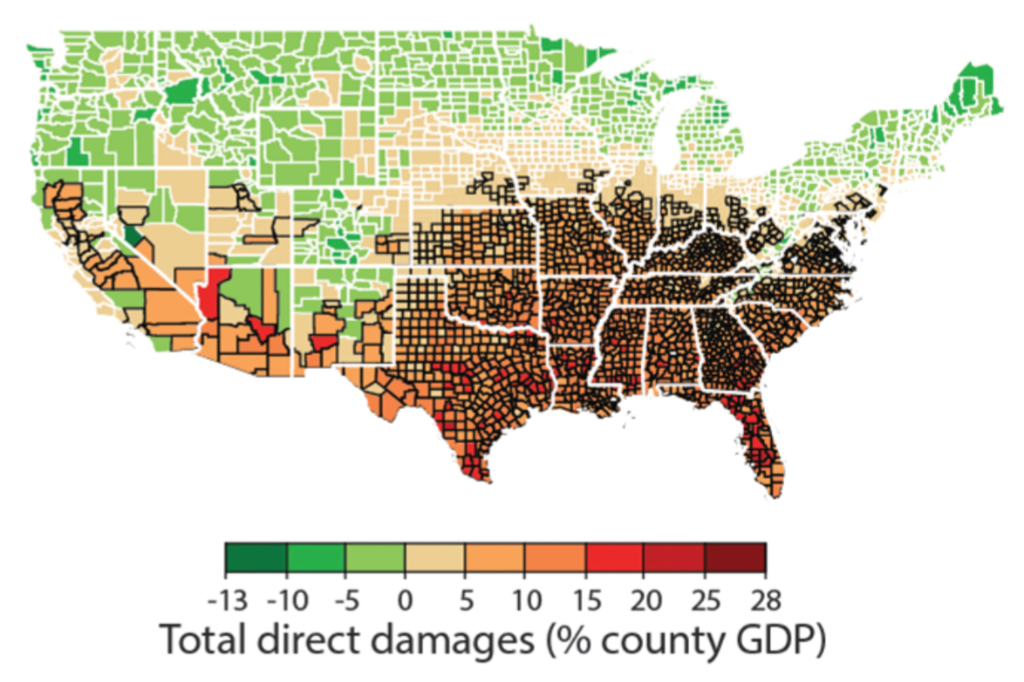
\includegraphics[width=\textwidth, height=0.50\textheight, keepaspectratio]{hsiang_map.png}\\
            \vspace{0.04cm}
            {\scriptsize County-level total direct damages (\% GDP) under RCP 8.5 (Hsiang et al., 2017).}
        \end{column}
    \end{columns}
\end{frame}

% SLIDE 4: FACT #3 — SPATIAL MACRO & THE DIMENSIONALITY CURSE
\begin{frame}{Fact \#3: Spatial Macro Models Struggle with Saving \hfill \hyperlink{backup:lit_taxonomy}{\scriptsize\beamergotobutton{Literature}}}\label{main:fact3}
    \begin{itemize}\small
        \item \textbf{The Curse of Dimensionality in Spatial Macroeconomics:}
        \begin{itemize}\footnotesize
            \item Standard dynamic spatial models (Desmet et al., 2018; Caliendo et al., 2019) capture forward-looking migration, but assume \textit{hand-to-mouth workers} or \textit{immobile capitalists} (Kleinman et al., 2023).
            \item Tracking the joint distribution of wealth and population across $J$ locations over time creates an intractable aggregate state space (Desmet, Nagy, Rossi-Hansberg, 2025).
        \end{itemize}
        \vspace{0.05cm}
        \item \textbf{Intertemporal Saving \& Distributional Impact:}
        \begin{itemize}\footnotesize
            \item Wealth accumulation provides vital self-insurance against uninsurable shocks (Caballero, 1990).
            \item Saving and migration interact dynamically: location acts as an asset (Bilal \& Rossi-Hansberg, 2021).
        \end{itemize}
        \vspace{0.05cm}
        \item \textbf{Computational Frontiers:}
        \begin{itemize}\footnotesize
            \item Recent efforts use deep neural networks (Sun, 2025) or OLG models (Giannone et al., 2023), but sacrifice analytical tractability and transparent policy decompositions.
        \end{itemize}
    \end{itemize}
    \vspace{0.08cm}
    \begin{tcolorbox}[takeawaybox, title=The Challenge]
        \footnotesize We need an \textbf{analytically tractable dynamic spatial model} where heterogeneous workers jointly choose consumption-saving and migration.
    \end{tcolorbox}
\end{frame}

% SLIDE 5: RESEARCH QUESTION & CONTRIBUTIONS
\begin{frame}{Research Question \& Contributions \hfill \hyperlink{backup:siam_comparison}{\scriptsize\beamergotobutton{S-IAM Comparison}}}\label{main:contributions}
    \begin{tcolorbox}[leafbox, title=Research Question]
        \small What are the aggregate and distributional impacts of climate change when individuals can both save and migrate, and how do these two adaptive margins interact?
    \end{tcolorbox}
    \vspace{0.06cm}
    {\small \textbf{Theoretical Foundation: Dvorkin \& Greaney (2025) (DG)}}
    \begin{itemize}\footnotesize
        \item Macro-finance spatial model with CARA preferences, Weibull preference shocks, and incomplete markets $\to$ yields closed-form decision rules and analytical independence of migration from wealth $a$.
    \end{itemize}
    \vspace{0.06cm}
    {\small \textbf{Three Core Extensions in this Paper:}}
    \begin{enumerate}\footnotesize\setlength{\itemsep}{2pt}
        \item \textit{Transitional Dynamics (2010--2500):} Explicitly solve 500-year dynamic transition path with backward induction and forward simulation (DG only compares static steady states).
        \item \textit{Empirical Climate Trajectory (2010--2100):} Map Hsiang et al. (2017) 6-sector damages into 3 structural channels: wages ($D^w$), amenities ($D^A$), and housing costs ($D^q$).
        \item \textit{Disentangling Moving Frictions \& Amenities:} 2-parameter gravity specification ($\psi_{\text{fix}}, \psi_{\text{dist}}$) breaks collinearity, isolating baseline amenities $\{A_\ell\}$.
    \end{enumerate}
\end{frame}

% =========================================================================
% SECTION 2: MODEL (SLIDES 6 TO 8)
% =========================================================================
\section{Model}

% SLIDE 6: ECONOMIC ENVIRONMENT (4 PILLARS)
\begin{frame}{Economic Environment: Spatial Structure, Risk, and Climate \hfill \hyperlink{backup:migration_frictions}{\scriptsize\beamergotobutton{US Mobility}}}\label{main:environment}
    \begin{enumerate}\small\setlength{\itemsep}{4pt}
        \item \textbf{Spatial Structure \& Geography:}
        \begin{itemize}\footnotesize
            \item $J = 51$ local labor markets (US States) with an associated wage $w_{t,j}$ and amenity $A_{t,j}$. Bilateral moving frictions: $\psi_{j\ell} = \psi_{\text{fix}} + \psi_{\text{dist}} \ln(1 + d_{j\ell})$ with $\psi_{jj}=0$.
            \item Idiosyncratic location preferences $\varepsilon \sim \text{i.i.d. Weibull}(\nu, \lambda)$ with shape $\nu$ governing migration elasticity.
        \end{itemize}
        \item \textbf{Income Processes \& Multiplicative Sorting:}
        \begin{itemize}\footnotesize
            \item Total labor earnings: $\tilde{w}_{j,t}(1 + z^\prime + \eta^\prime)$ with persistent shock $z^\prime = \rho z + \epsilon^\prime$ ($\epsilon \sim \mathcal{N}(0, \sigma_{\epsilon,\ell}^2)$) and transitory shock $\eta \sim \mathcal{N}(0, \sigma_{\eta,\ell}^2)$. High-$z$ workers gain proportionally more in high-wage states $\implies$ generates spatial sorting.
        \end{itemize}
        \item \textbf{Incomplete Financial Markets:}
        \begin{itemize}\footnotesize
            \item No state-contingent claims against $(z^\prime, \eta^\prime, \varepsilon)$. Single risk-free bond with constant interest rate $r$. Self-insurance operates solely via risk-free wealth $a$ at price $\frac{1}{1+r}$ that yields one unit of consumption next period.
        \end{itemize}
        \item \textbf{Climate Change Shocks (2010--2100):}
        \begin{itemize}\footnotesize
            \item Exogenous permanent damage paths from Hsiang et al. (2017) across 3 channels: wages $w_{\ell,t} = w_{\ell,0}(1 - D^w_{\ell,t})$, amenities $A_{\ell,t} = A_{\ell,0}(1 - D^A_{\ell,t})$, and housing expenditures $q_{\ell,t} = q_{\ell,0}(1 + D^q_{\ell,t})$.
        \end{itemize}
    \end{enumerate}
\end{frame}

% SLIDE 7: AGENT PREFERENCES, BUDGET CONSTRAINT & TIMING
\begin{frame}{Model: Preferences, Budget Constraint, and Timing \hfill \hyperlink{backup:rouwenhorst}{\scriptsize\beamergotobutton{Income Process}}}\label{main:preferences}
    \begin{itemize}\small\setlength{\itemsep}{3pt}
        \item \textbf{Preferences \& Demographics:}
        $$u(c_{j,t}, A_{j,t}) = -\tfrac{1}{\gamma} \exp\left(-\gamma c_{j,t} - \tilde{A}_{j,t}\right), \quad \tilde{A}_{j,t} = A_{j,t}(1 - D^A_{j,t})$$
        Annual turnover death rate $\delta$ (Blanchard-Yaari); newborns arrive with $a^0 = 0, z=0$.
        \item \textbf{Flow Budget Constraint:}
        $$c_{j,t} + \tfrac{a_{j,t+1}}{1 + r} = \tilde{y}_{j,t} + \tilde{w}_{j,t}(z^\prime + \eta^\prime) + a$$
        where effective wage is $\tilde{w}_{j,t} \equiv w_{j,t}(1-D^w_{j,t})$ and disposable income is $\tilde{y}_{j,t} \equiv \tilde{w}_{j,t} - q_{j,t}(1+D^q_{j,t})$.
        \item \textbf{Intra-Period 6-Step Sequence} (\textit{bold indicates agent choice}):
        \begin{enumerate}\footnotesize\setlength{\itemsep}{1pt}
            \item Enter period in location $j$ with wealth $a$ and past productivity $z$.
            \item Observe fundamentals, draw preference shocks $\boldsymbol{\varepsilon} \in \mathbb{R}^J_+$, and observe $(w, A, q)$.
            \item \textbf{Choose destination location} $\ell \in \{1,\dots,J\}$ facing moving friction $\psi_{j\ell}$.
            \item Realize destination income shocks $(z^\prime, \eta^\prime)$ in location $\ell$.
            \item \textbf{Choose consumption and savings} ($c_{\ell,t}, a_{\ell,t+1}$).
            \item Survive with probability $1-\delta$; die with probability $\delta$, replaced by newborn ($a^0=0, z=0$).
        \end{enumerate}
    \end{itemize}
    \vspace{0.06cm}
\end{frame}

% SLIDE 8: PROPOSITION 1 — CLOSED-FORM POLICIES
\begin{frame}{Closed-Form Policies and Tractability \hfill \hyperlink{backup:prop1_proof}{\scriptsize\beamergotobutton{Proof \& Ex-Ante}}}\label{main:prop1}
    \begin{itemize}\small\setlength{\itemsep}{2pt}
        \item \textbf{1. Closed-Form Consumption and Asset Policies:}
        \begin{align*}
        c_{\ell,t}(a, z^\prime, \eta^\prime) &= \Xi_{\ell,t}(z^\prime) + \tfrac{r}{1+r} \left[ \tilde{y}_{\ell,t} + \tilde{w}_{\ell,t}\eta^\prime + a \right] \\
        a_{\ell,t+1}(a, z^\prime, \eta^\prime) &= \tilde{y}_{\ell,t} + \tilde{w}_{\ell,t}\eta^\prime + a + (1+r)(\tilde{w}_{\ell,t}z^\prime - \Xi_{\ell,t}(z^\prime))
        \end{align*}
        \item \textbf{2. Bilateral Migration Probability Policy:}
        $$\mu_{j\ell,t}(z) = \frac{ \exp\left(\nu \mathbb{B}_{1,j\ell,t}\right) \left(\mathbb{E}_{z^\prime | z, \ell} \left[ e^{-\gamma \Xi_{\ell,t}(z^\prime)} \right]\right)^{-\nu} }{ \sum_{m=1}^J \exp\left(\nu \mathbb{B}_{1,jm,t}\right) \left(\mathbb{E}_{z^\prime | z, m} \left[ e^{-\gamma \Xi_{m,t}(z^\prime)} \right]\right)^{-\nu} }$$
        where $\mathbb{B}_{1,j\ell,t} = \tilde{A}_{\ell,t} - \psi_{j\ell} + \frac{\gamma r \tilde{y}_{\ell,t}}{1+r} - \frac{1}{2}\left(\frac{\gamma r \tilde{w}_{\ell,t}}{1+r}\right)^2 \sigma_{\eta,\ell}^2$.
    \end{itemize}
    \vspace{0.02cm}
    \begin{tcolorbox}[takeawaybox, title=Tractability Breakthrough]
        \footnotesize
        \begin{itemize}\setlength{\itemsep}{1pt}
            \item Continuation value $\Xi_{\ell,t}(z^\prime)$ and mobility shares $\mu_{j\ell,t}(z)$ are strictly independent of financial wealth $a$. Aggregate state space collapses from $(a, z, \ell)$ to $(z, \ell)$ (no curse of dimensionality).
        \end{itemize}
    \end{tcolorbox}
\end{frame}


\begin{frame}{$\Xi$ Recursion \& Certainty Equivalent Welfare Metric \label{backup:xi_ce_metric}}
    \begin{columns}[T]
        \begin{column}{0.485\textwidth}
            \textbf{\small Value Function Index $\Xi_{\ell,t}(z)$}
            \vspace{0.04cm}
            \begin{itemize}\scriptsize\setlength{\itemsep}{2pt}
                \item Factorized Ex-Ante Value Function:
                $$v_{\ell,t}(a, z) = \mathbb{E}_\varepsilon(V_{\ell,t}(z)) = -\tfrac{1}{\gamma} \exp\left( -\gamma \left[ \tfrac{r}{1+r} a + \Xi_{\ell,t}(z) \right] \right)$$
                \item $\Xi$ Recursion:
                {\tiny
                \begin{align*}
\Xi_{\ell,t}(z) &= \underbrace{\tfrac{r \tilde{w}_{\ell,t} z}{1+r}}_{\text{Current Income}} - \underbrace{\tfrac{\tilde{A}_{\ell,t} + \ln \bar{\lambda}}{\gamma(1+r)}}_{\text{Current Amenities}} \\
&\quad + \underbrace{\begin{aligned}
    &\tfrac{1}{\gamma\nu(1+r)} \ln \sum_{m=1}^J \exp\Bigl( \nu \mathbb{B}_{1,\ell m, t+1} \\
    &\qquad - \nu \ln \mathbb{E}_{z'|z,m}[e^{-\gamma \Xi_{m,t+1}(z')}] \Bigr)
\end{aligned}}_{\text{Future Spatial Option Value}}
\end{align*}
                }
                \item \textbf{Economic Role:}
                \begin{itemize}\tiny
                    \item Non-assetconsumption intercept ($c = \Xi + \kappa[a + \tilde{y} + \tilde{w}\eta']$).
                    \item Summarizes future wages, amenities, and spatial mobility option value.
                    \item Strictly independent of assets $a \to$ state space collapses from 3D to 2D.
                \end{itemize}
            \end{itemize}
        \end{column}
        
        \begin{column}{0.495\textwidth}
            \textbf{\small Certainty Equivalent Welfare Metric}
            \vspace{0.04cm}
            \begin{itemize}\scriptsize\setlength{\itemsep}{2pt}
                \item Individual Certainty Equivalent ($\text{CE}$):
                $$\text{CE}_{\ell,t}(a, z) = \kappa a + \Xi_{\ell,t}(z), \quad \kappa \equiv \tfrac{r}{1+r}$$
                \item State \& National Aggregation:
                {\tiny
                \begin{align*}
                \overline{\text{CE}}_{\ell,t} &= \tfrac{1}{L_{\ell,t}} \sum_{z=1}^{N_z} \Lambda_t(\ell, z) \left[ \kappa \bar{a}_t(\ell, z) + \Xi_{\ell,t}(z) \right] \\
                \text{CE}_t^{\text{agg}} &= \sum_{\ell=1}^J L_{\ell,t} \overline{\text{CE}}_{\ell,t}
                \end{align*}
                }
                \item Consumption Equivalent Variation ($\lambda_{\text{nat}}$):
                {\tiny
                $$\lambda_{\text{nat}, t} = \frac{\sum_{\ell=1}^J (\overline{\text{CE}}_{\ell,t} - \overline{\text{CE}}_\ell^{\text{init}}) \Lambda_{\ell,t}}{\sum_{\ell=1}^J c_\ell^{\text{init}} \Lambda_\ell^{\text{init}}}$$
                }
            \end{itemize}
        \end{column}
    \end{columns}
\end{frame}

% =========================================================================
% SECTION 3: SAVING MOTIVES & WEALTH ACCUMULATION (SLIDES 9 TO 12)
% =========================================================================
\section{Saving Rule \& Wealth Accumulation}

% SLIDE 9: DETERMINISTIC BASELINE & DAMAGE SMOOTHING
\begin{frame}{Saving Motives: Deterministic Baseline \& Damage Smoothing \hfill \hyperlink{backup:shift_share_algo}{\scriptsize\beamergotobutton{Shift-Share}}}\label{main:saving_det}
    \begin{itemize}\small\setlength{\itemsep}{4pt}
        \item \textbf{Setting:} Immobile autarky ($J = 1$) without idiosyncratic income shocks ($z = 0, \eta = 0$).
        \item \textbf{The Incremental Climate Damage Smoothing Saving Rule:}
        \begin{equation}
        \Delta a_{t+1} = \sum_{s=0}^{\infty} \frac{1}{(1+r)^s} \left[ \underbrace{w \Delta D^w_{t+s+1}}_{\text{Wage loss smoothing}} + \underbrace{q \Delta D^q_{t+s+1}}_{\text{Housing cost smoothing}} + \underbrace{\tfrac{A}{\gamma} \Delta D^A_{t+s+1}}_{\text{Amenity loss smoothing}} \right]
        \label{eq:saving_smooth}
        \end{equation}
        where $\Delta D_{t+s+1} = D_{t+s+1} - D_{t+s}$ is the incremental annual climate shock degradation.
    \end{itemize}
    \vspace{0.15cm}
    \begin{tcolorbox}[takeawaybox, title=Economic Takeaway]
        \small Precautionary asset accumulation is driven strictly by the \textbf{growth rate / ramp of damages} ($\Delta D$). Once climate damages stabilize ($\Delta D = 0$), deterministic accumulation ceases ($\Delta a_{t+1} = 0$).
    \end{tcolorbox}
\end{frame}

% SLIDE 10: INCOME RISK & DAMAGE-LEVEL DAMPENING
\begin{frame}{Saving Motives: Income Risk and Damage-Level Dampening \hfill \hyperlink{backup:uncertainty_var}{\scriptsize\beamergotobutton{Variance Risk}}}\label{main:saving_risk}
    \begin{itemize}\footnotesize\setlength{\itemsep}{2pt}
        \item Persistent AR(1) shock $z^\prime = \rho z + \epsilon^\prime$ and transitory shock $\eta^\prime$. Disposable income: $\tilde{Y}_{t+s} = \tilde{y}_{t+s} + \tilde{w}_{t+s} z_{t+s} + \tilde{w}_{t+s}\eta_{t+s}$.
        \item \textbf{General Stochastic Saving Rule:}
        \begin{equation}
        \Delta a_{t+1}(z) = \sum_{s=0}^{\infty} \frac{1}{(1+r)^s} \left[ \left(\mathbb{E}_t[\tilde{Y}_{t+s}] - \mathbb{E}_t[\tilde{Y}_{t+s+1}]\right) + \tfrac{1}{\gamma} (A_{t+s} - A_{t+s+1}) + \textcolor{mutedgold}{\mathbf{\tfrac{\gamma}{2} \sigma_{C, t+s+1}^2 \quad \text{\small (2)}}} \right]
        \label{eq:saving_stoch}
        \end{equation}
        where innovation variance is $\sigma_{C, t+s}^2 = \left( \tfrac{r}{1+r} \tilde{w}_{t+s} \right)^2 \sigma_{\eta, t+s}^2 + \Omega_{t+s}^2 \sigma_{\epsilon, t+s}^2$.
        \item \textbf{Expected Income Drop Decomposition:}
        \begin{equation}
        \mathbb{E}_t[\tilde{Y}_{t+s}] - \mathbb{E}_t[\tilde{Y}_{t+s+1}] = w \Delta D^w_{t+s+1} (1 + z_t \rho^{s+1}) + q \Delta D^q_{t+s+1} + z_t \rho^s (1 - \rho) w - \textcolor{terracotta}{\mathbf{z_t \rho^s (1 - \rho) w D^w_{t+s} \quad \text{\small (1)}}}
        \label{eq:income_drop}
        \end{equation}
    \end{itemize}
    \vspace{0.04cm}
    \begin{tcolorbox}[takeawaybox, title=Two Competing Income Risk Motives]
        \footnotesize
        \begin{itemize}\setlength{\itemsep}{1pt}
            \item \textcolor{terracotta}{\textbf{(1) Damage Dampening Effect:}} Accumulated damages $D^w$ permanently depress base wages, contracting the dollar spread of mean-reversion and \textit{depressing} target savings.
            \item \textcolor{mutedgold}{\textbf{(2) Precautionary Risk Motive:}} Uninsurable income risk generates positive precautionary savings  ($\frac{\gamma}{2} \sigma_C^2$).
        \end{itemize}
    \end{tcolorbox}
\end{frame}

% SLIDE 11: SPATIAL OPTION VALUE & ADAPTIVE MARGINS
\begin{frame}{Saving Motives: Spatial Option Value \& Adaptive Margins \hfill \hyperlink{backup:ushape}{\scriptsize\beamergotobutton{U-Shape Sweep}}}\label{main:saving_option}
    \begin{itemize}\small\setlength{\itemsep}{2pt}
        \item \textbf{Setting:} Multi-location spatial economy ($J = 51$), abstracting from idiosyncratic income risk.
        \item \textbf{Saving Rule with Spatial Option Value:}
        \begin{equation}
        \Delta a_{\ell, t+1} = \sum_{s=0}^{\infty} \frac{1}{(1+r)^s} \left[ (\tilde{y}_{\ell, t+s} - \tilde{y}_{\ell, t+s+1}) + \tfrac{1}{\gamma} (A_{\ell, t+s} - A_{\ell, t+s+1}) + \textcolor{emerald}{\mathbf{\tfrac{1}{\gamma \nu} \ln \mu_{\ell \ell, t+s} \quad \text{\small (3)}}} \right]
        \label{eq:saving_spatial}
        \end{equation}
        where \textcolor{emerald}{\textbf{(3) Spatial Option Value}} enters with $\ln \mu_{\ell\ell,t+s} \le 0$ because staying probability $\mu_{\ell\ell} \le 1$.
    \end{itemize}
    \vspace{0.04cm}
    \begin{columns}[T]
        \begin{column}{0.48\textwidth}
            \begin{tcolorbox}[leafbox, title=Substitutability (Spatial Insurance)]
                \scriptsize
                \begin{itemize}\setlength{\itemsep}{1pt}
                    \item \textbf{Damaged states:} Fundamentals drop $\implies \mu_{\ell\ell} \downarrow \implies \ln \mu_{\ell\ell}$ more negative $\implies$ substitute to migration, \textbf{save less}.
                    \item \textbf{Haven states:} Outside options worsen $\implies \mu_{\ell\ell} \to 1 \implies \ln \mu_{\ell\ell} \to 0 \implies$ spatial insurance vanishes, \textbf{save more}.
                \end{itemize}
            \end{tcolorbox}
        \end{column}
        \begin{column}{0.48\textwidth}
            \begin{tcolorbox}[leafbox, title=Complementarity (Taste Buffering)]
                \scriptsize
                \begin{itemize}\setlength{\itemsep}{1pt}
                    \item Drawing a strong idiosyncratic preference shock $\varepsilon$ for a lower-wage/damaged state requires financial savings to smooth consumption.
                \end{itemize}
            \end{tcolorbox}
        \end{column}
    \end{columns}
\end{frame}

% SLIDE 12: THE 5 MECHANISMS ACROSS STEADY STATES
\begin{frame}{Wealth Accumulation: The 5 Mechanisms Across Steady States}\label{main:mechanisms}
    \begin{itemize}\footnotesize\setlength{\itemsep}{1pt}
        \item \textbf{Cross-Steady-State Intensive Margin:}
        \begin{equation}
        \Delta a_\ell^{\text{Saving Rule}}(z) \propto \sum_{s=0}^{\infty} \frac{1}{(1+r)^s} \left[ \underbrace{- z \rho^s (1-\rho) w \Delta^{SS} D^w_\ell}_{\text{\textcolor{terracotta}{(1) Damage Dampening}}} + \underbrace{\tfrac{\gamma}{2} \Delta^{SS} \sigma_{C, \ell}^2}_{\text{\textcolor{mutedgold}{(2) Precautionary Risk}}} + \underbrace{\tfrac{1}{\gamma \nu} \Delta^{SS} \ln \mu_{\ell \ell}(z)}_{\text{\textcolor{emerald}{(3) Spatial Option Value}}} \right]
        \label{eq:intensive_margin}
        \end{equation}
        \item \textbf{State-Level Shift-Share Wealth Decomposition:}
        \begin{equation}
        \Delta^{SS} \bar{a}_\ell = \sum_z \pi_\ell^{\text{init}}(z) \big[\Delta a_\ell^{\text{Saving Rule}}(z) + \underbrace{\Delta a_\ell^{\text{Transition}}(z)}_{\text{\textcolor{lightemerald}{\textbf{(4) Spatial Transition}}}}\big] + \underbrace{\sum_z \big[\pi_\ell^{\text{term}}(z) - \pi_\ell^{\text{init}}(z) \big] a_\ell^{\text{term}}(z)}_{\text{\textcolor{cobaltblue}{\textbf{(5) Compositional Sorting}}}}
        \label{eq:shift_share}
        \end{equation}
    \end{itemize}
    \vspace{0.04cm}
    \begin{tcolorbox}[leafbox, title=Recap of the 5 Mechanisms]
        \scriptsize
        \begin{columns}[T]
            \begin{column}{0.50\textwidth}
                \begin{enumerate}\setlength{\itemsep}{0pt}
                    \item \textcolor{terracotta}{\textbf{(1) Damage Dampening:}} Lower base wages reduce spread of mean-reversion $\to$ depresses savings.
                    \item \textcolor{mutedgold}{\textbf{(2) Precautionary Risk:}} Shifts in variance $\Delta \sigma_C^2 \to$ alters precautionary wealth target.
                    \item \textcolor{emerald}{\textbf{(3) Spatial Option Value:}} Changes in $\ln \mu_{\ell\ell} \to$ adjusts spatial insurance substitution.
                \end{enumerate}
            \end{column}
            \begin{column}{0.48\textwidth}
                \begin{enumerate}\setcounter{enumi}{3}\setlength{\itemsep}{0pt}
                    \item \textcolor{lightemerald}{\textbf{(4) Spatial Transition:}} Inflow of migrants carrying historical wealth from origin.
                    \item \textcolor{cobaltblue}{\textbf{(5) Compositional Sorting:}} Selective sorting of high-$z$ workers shifts demographic composition.
                \end{enumerate}
            \end{column}
        \end{columns}
    \end{tcolorbox}
\end{frame}

% =========================================================================
% SECTION 4: CALIBRATION & DAMAGES (SLIDES 13 TO 14)
% =========================================================================
\section{Calibration \& Damages}

% SLIDE 13: CALIBRATION & NU IDENTIFICATION
\begin{frame}{Calibration: Internal vs. External Identification \hfill \hyperlink{backup:data_sources}{\scriptsize\beamergotobutton{Data Sources}} \hyperlink{backup:param_table}{\scriptsize\beamergotobutton{Parameters}}}\label{main:calibration}
    \begin{columns}[T]
        \begin{column}{0.48\textwidth}
            \textbf{Externally Set Parameters (Dvorkin \& Greaney, 2025):}
            \begin{itemize}\small\setlength{\itemsep}{1pt}
                \item Wages $\{w_\ell\}$, shock variances $\{\sigma_{\epsilon,\ell}^2, \sigma_{\eta,\ell}^2\}$ from CPS-ORG \& IRS SOI
                \item Macro parameters: $r = 0.03$, $\beta = 1/(1+r) = 0.971$, $\gamma = 3.0$, $\delta = 0.025$, $\rho = 0.934$, $\alpha_h = 0.30$
                \item Migration elasticity: $\nu = 3.95$ \textit{(DG 2025, Caliendo et al. 2019)}
            \end{itemize}
            \vspace{0.06cm}
            \textbf{Internally Calibrated (Nested Loop):}
            \begin{itemize}\small\setlength{\itemsep}{1pt}
                \item Outer loop $\psi_{\text{fix}} = 1.633$ matches empirical inter-state migration rate, $\psi_{\text{dist}} = 0.405$ the average distance of migration, $\bar{\lambda} = 0.371$ the empirical Wealth-to-Earnings ratio.
                \item Inner loop mapping: Amenities $\{A_\ell\}$ match population shares
            \end{itemize}
        \end{column}
        \begin{column}{0.50\textwidth}
            \begin{tcolorbox}[leafbox, title=The Identification Challenge of $\nu$]
                \footnotesize
                \begin{itemize}\setlength{\itemsep}{1.5pt}
                    \item Bilateral moving costs use 2-parameter gravity:
                    $$\psi_{j\ell} = \psi_{\text{fix}} + \psi_{\text{dist}} \ln(1 + d_{j\ell})$$
                    \item \textbf{Collinearity break:} Separates $\psi_{j\ell}$ from baseline amenities $A_\ell$.
                    \item Why fix $\nu = 3.95$ externally? Smooth gravity cannot fit idiosyncratic asymmetric flows. Internal calibration of $\nu$ would force $\nu \downarrow 2.16$, injecting artificial noise to fit spatial sorting.
                    \item Fixing $\nu = 3.95$ preserves a realistic macroeconomic migration elasticity to climate shocks.
                \end{itemize}
            \end{tcolorbox}
        \end{column}
    \end{columns}
\end{frame}

% SLIDE 14: CLIMATE DAMAGE MAPPING (HSIANG ET AL. 2017)
\begin{frame}{Climate Damage Mapping: 6 Sectors into 3 Channels \hfill \hyperlink{backup:damage_channels}{\scriptsize\beamergotobutton{Damage Channels}}}\label{main:damage_mapping}
    \textbf{\small Sector-to-Channel Mapping Equations (Hsiang et al., 2017):}
    \vspace{-0.1cm}
    \begin{itemize}\footnotesize\setlength{\itemsep}{1pt}
        \item \textbf{Wage Channel:} $\Delta w_\ell = \frac{\bar L_\ell}{100} + \frac{\bar Y_\ell^{\text{agri}}}{100} s_\ell^{\text{agri}} - \frac{\bar C_\ell}{100}$ \quad \textit{(Labor productivity $\bar{L}_\ell$, Agriculture $\bar{Y}_\ell^{\text{agri}}$, Coastal storms $\bar{C}_\ell$)}
        \item \textbf{Amenity Channel:} $\Delta A_\ell = \gamma \left[ \frac{\bar M_\ell}{10^5} \frac{\text{VSL}}{\bar Y_{\text{US}}} + \frac{\bar R_\ell}{10^5} \frac{\mathbb{E}[\text{VSC}]}{\bar Y_{\text{US}}} \right]$ \quad \textit{(Mortality $\bar{M}_\ell$ [VSL=\$9M], Crime $\bar{R}_\ell$ [VSC], $\bar Y_{\text{US}}=\$48.7\text{k}$)}
        \item \textbf{Housing Channel:} $\Delta q_\ell = \frac{\bar E_\ell}{100} s_\ell^{\text{energy}}$ \quad \textit{(Energy expenditure share)}
    \end{itemize}
    \vspace{0.04cm}
    \textbf{\footnotesize Spatial Damage Distribution (at 2100):}
    \vspace{0.02cm}
    \begin{center}
        \begin{minipage}{0.32\textwidth}
            \centering
            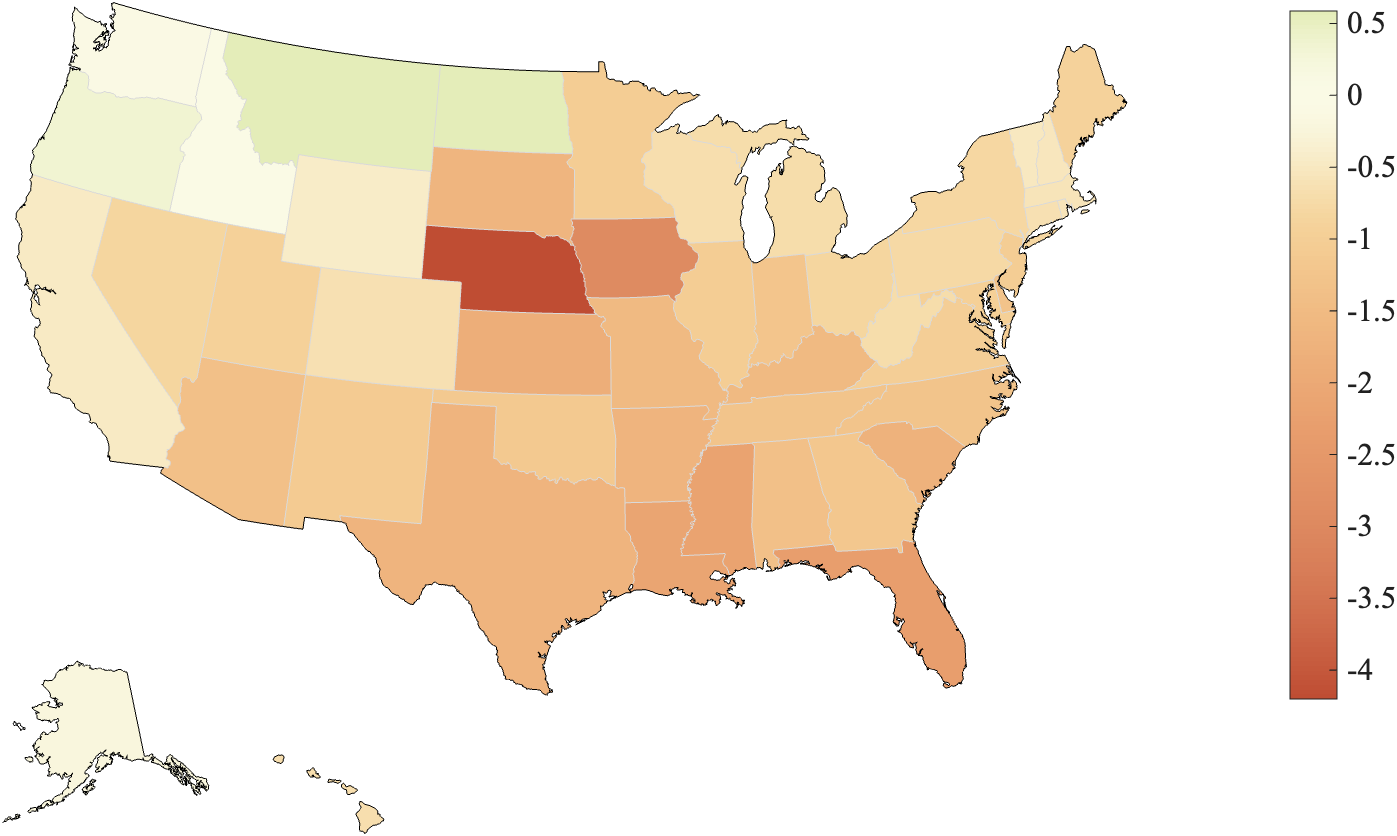
\includegraphics[width=\textwidth, height=0.34\textheight, keepaspectratio]{../Output/big_nu/graph_perfect_foresight/damage_maps/damage_maps_damage_wage.png}\\
            \vspace{0.02cm}
            {\scriptsize \textbf{(a) Wage Damage ($\Delta w_\ell$ [\%])}}
        \end{minipage}\hfill
        \begin{minipage}{0.32\textwidth}
            \centering
            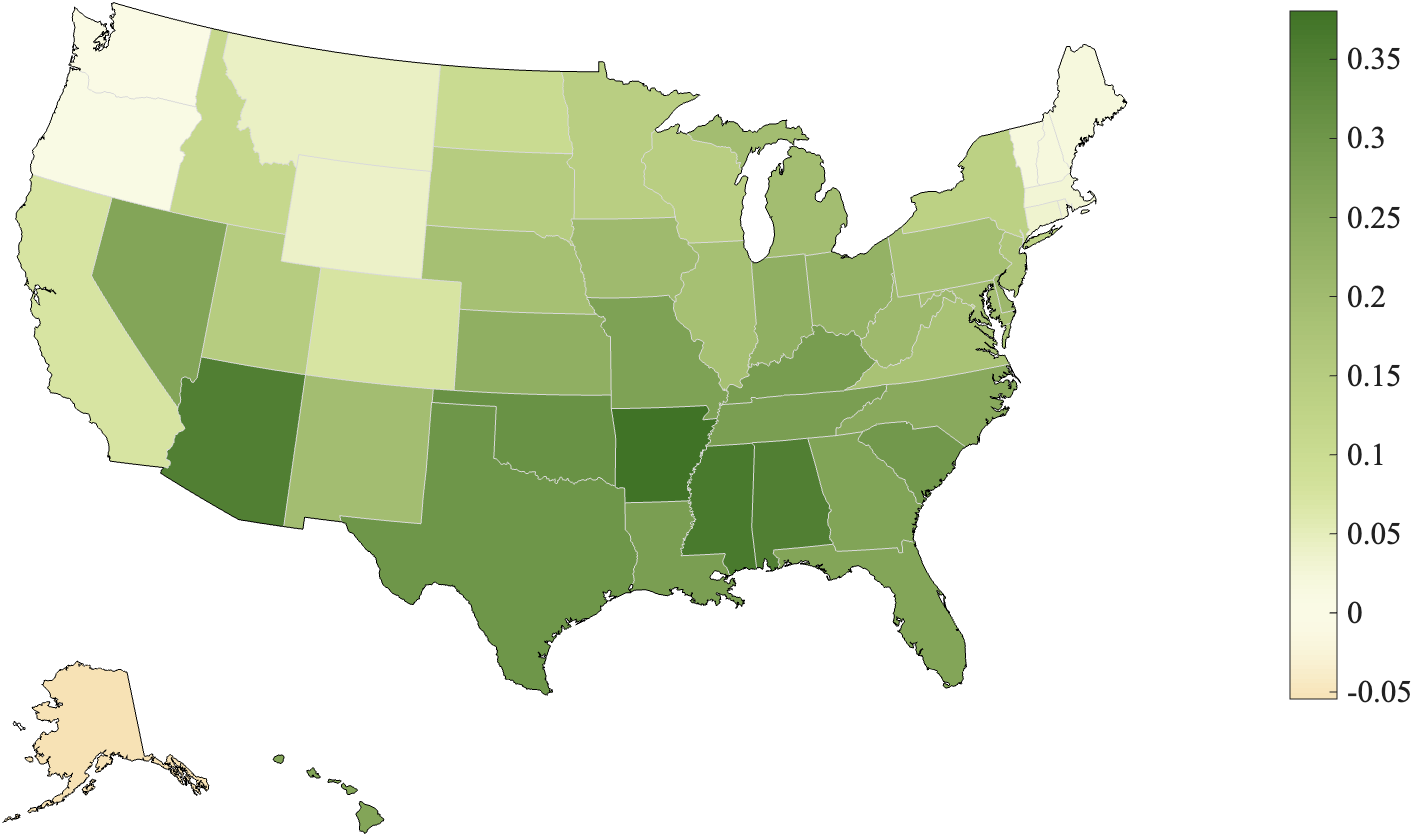
\includegraphics[width=\textwidth, height=0.34\textheight, keepaspectratio]{../Output/big_nu/graph_perfect_foresight/damage_maps/damage_maps_damage_housing.png}\\
            \vspace{0.02cm}
            {\scriptsize \textbf{(b) Housing Cost Damage ($\Delta q_\ell$ [\%])}}
        \end{minipage}\hfill
        \begin{minipage}{0.32\textwidth}
            \centering
            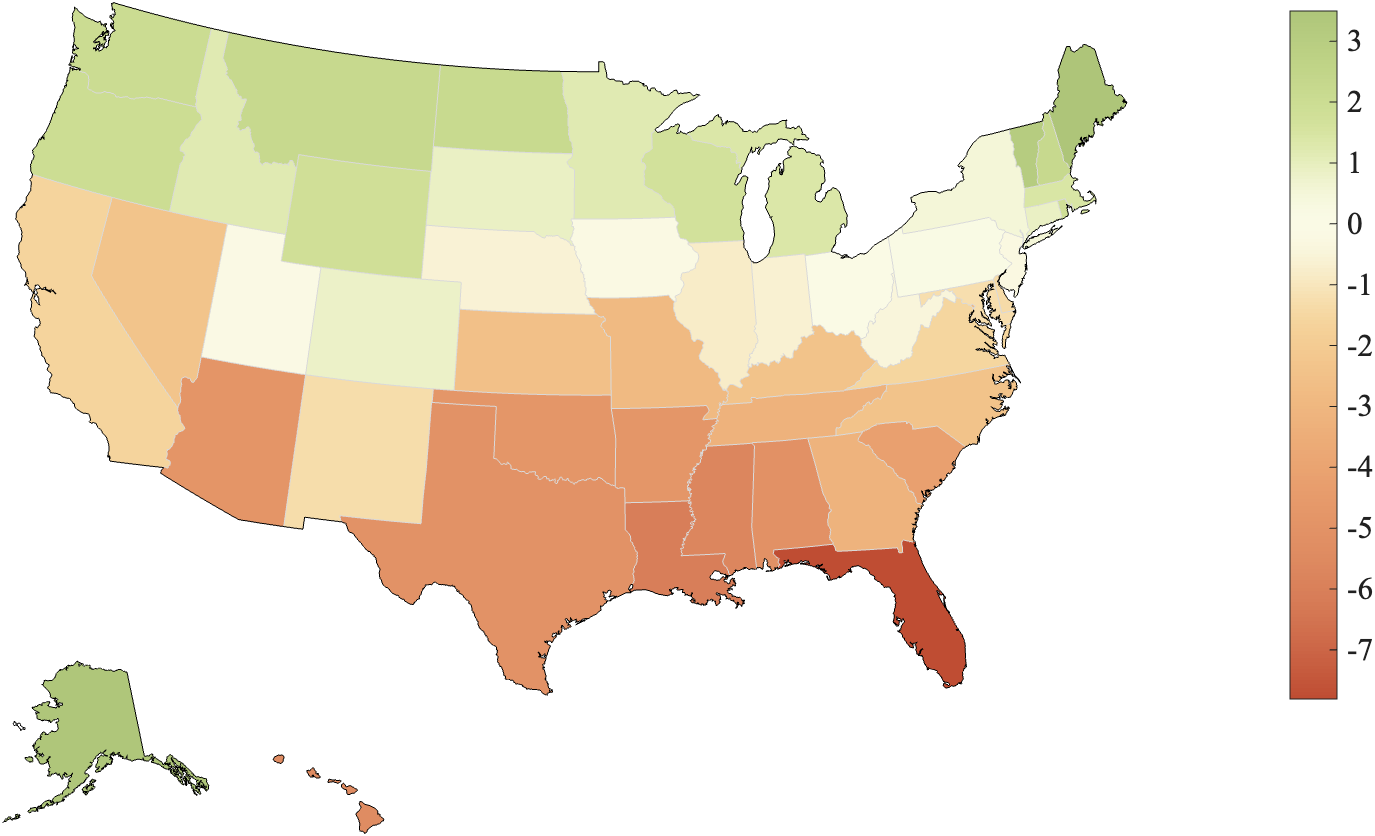
\includegraphics[width=\textwidth, height=0.34\textheight, keepaspectratio]{../Output/big_nu/graph_perfect_foresight/damage_maps/damage_maps_damage_amenity.png}\\
            \vspace{0.02cm}
            {\scriptsize \textbf{(c) Amenity Damage ($\Delta A_\ell$ [\% Equiv.])}}
        \end{minipage}
    \end{center}
\end{frame}

% =========================================================================
% SECTION 5: QUANTITATIVE RESULTS (SLIDES 15 TO 19)
% =========================================================================
\section{Quantitative Results}

% SLIDE 15: NATIONAL AGGREGATE DYNAMICS (3 TIME SERIES)
\begin{frame}{National Aggregate Dynamics: Precautionary Saving \& Sorting \hfill \hyperlink{backup:solution_algo}{\scriptsize\beamergotobutton{Algorithm}} \hyperlink{backup:peak_maps}{\scriptsize\beamergotobutton{Peak Maps}}}\label{main:agg_dynamics}
    \begin{columns}[T]
        \begin{column}{0.33\textwidth}
            \centering
            \textbf{\footnotesize (a) Earnings ($Y_t$ [Normalized])}\\
            \vspace{0.04cm}
            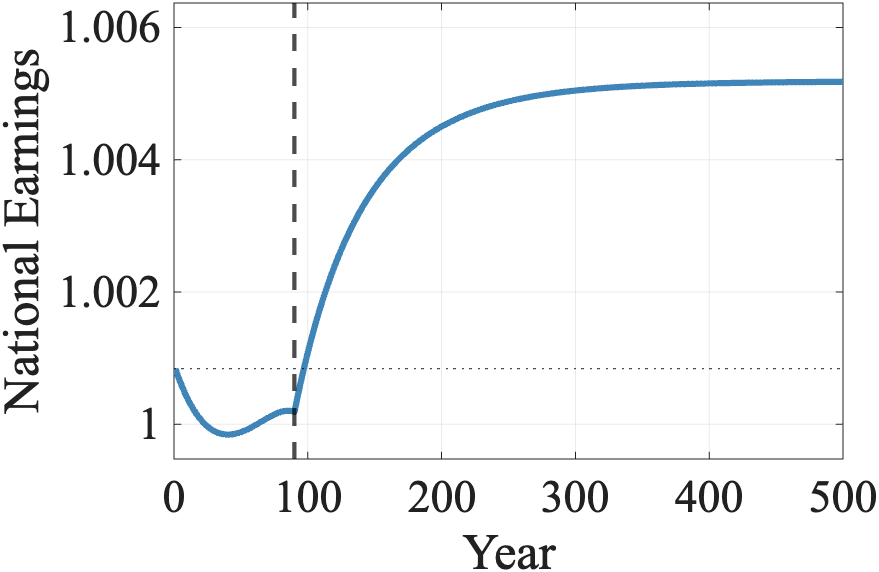
\includegraphics[width=\textwidth]{../Output/big_nu/graph_perfect_foresight/dynamic_moments/dynamic_moments_national_earnings.png}
            \vspace{-0.15cm}
            \begin{itemize}\scriptsize\setlength{\itemsep}{1pt}
                \item Falls $-0.2\%$ initially.
                \item Rises $+0.4\%$ ($+\$250/\text{yr}$) by 2100 as workers sort into higher-wage Northern states.
            \end{itemize}
        \end{column}
        \begin{column}{0.33\textwidth}
            \centering
            \textbf{\footnotesize (b) Total Wealth ($W_t$)}\\
            \vspace{0.04cm}
            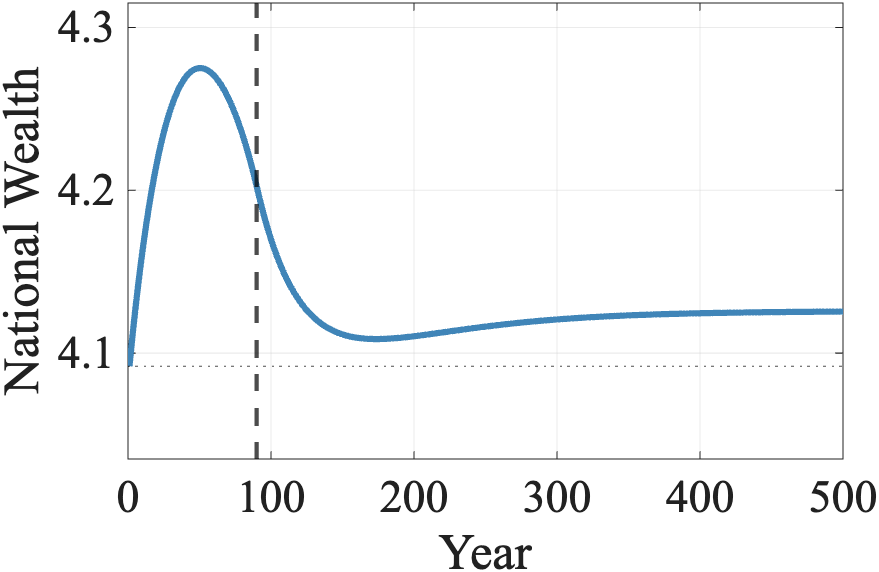
\includegraphics[width=\textwidth]{../Output/big_nu/graph_perfect_foresight/dynamic_moments/dynamic_moments_national_wealth.png}
            \vspace{-0.15cm}
            \begin{itemize}\scriptsize\setlength{\itemsep}{1pt}
                \item \textbf{Precautionary peak:} $+4.5\%$ wealth accumulation by 2090.
                \item Decumulates over 300-year transition to smooth consumption.
            \end{itemize}
        \end{column}
        \begin{column}{0.33\textwidth}
            \centering
            \textbf{\footnotesize (c) Migration Rate ($m_t$ [Share])}\\
            \vspace{0.04cm}
            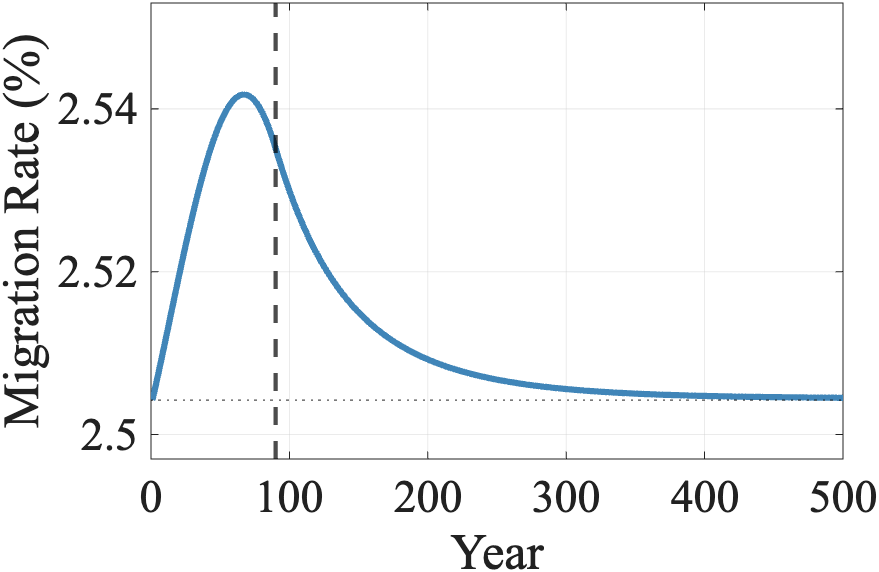
\includegraphics[width=\textwidth]{../Output/big_nu/graph_perfect_foresight/dynamic_moments/dynamic_moments_national_mobility.png}
            \vspace{-0.15cm}
            \begin{itemize}\scriptsize\setlength{\itemsep}{1pt}
                \item Slight rise from $2.50\%$ to $2.60\%$ during peak shock ramp.
                \item Small aggregate change hides huge cumulative state reallocation.
            \end{itemize}
        \end{column}
    \end{columns}

\end{frame}

% SLIDE 16: SPATIAL HETEROGENEITY (MAPS)
\begin{frame}{Spatial Heterogeneity: Population Flight \& Wealth Destruction \hfill \hyperlink{backup:inequality_dynamics}{\scriptsize\beamergotobutton{Inequality}} \hyperlink{backup:xi_mechanics}{\scriptsize\beamergotobutton{$\Xi$ Gradients}}}\label{main:spatial_hetero}
    \begin{columns}[T]
        \begin{column}{0.48\textwidth}
            \centering
            \textbf{\small Local Population Change ($\Delta \text{Pop}_\ell$ [\%])}\\
            \vspace{0.04cm}
            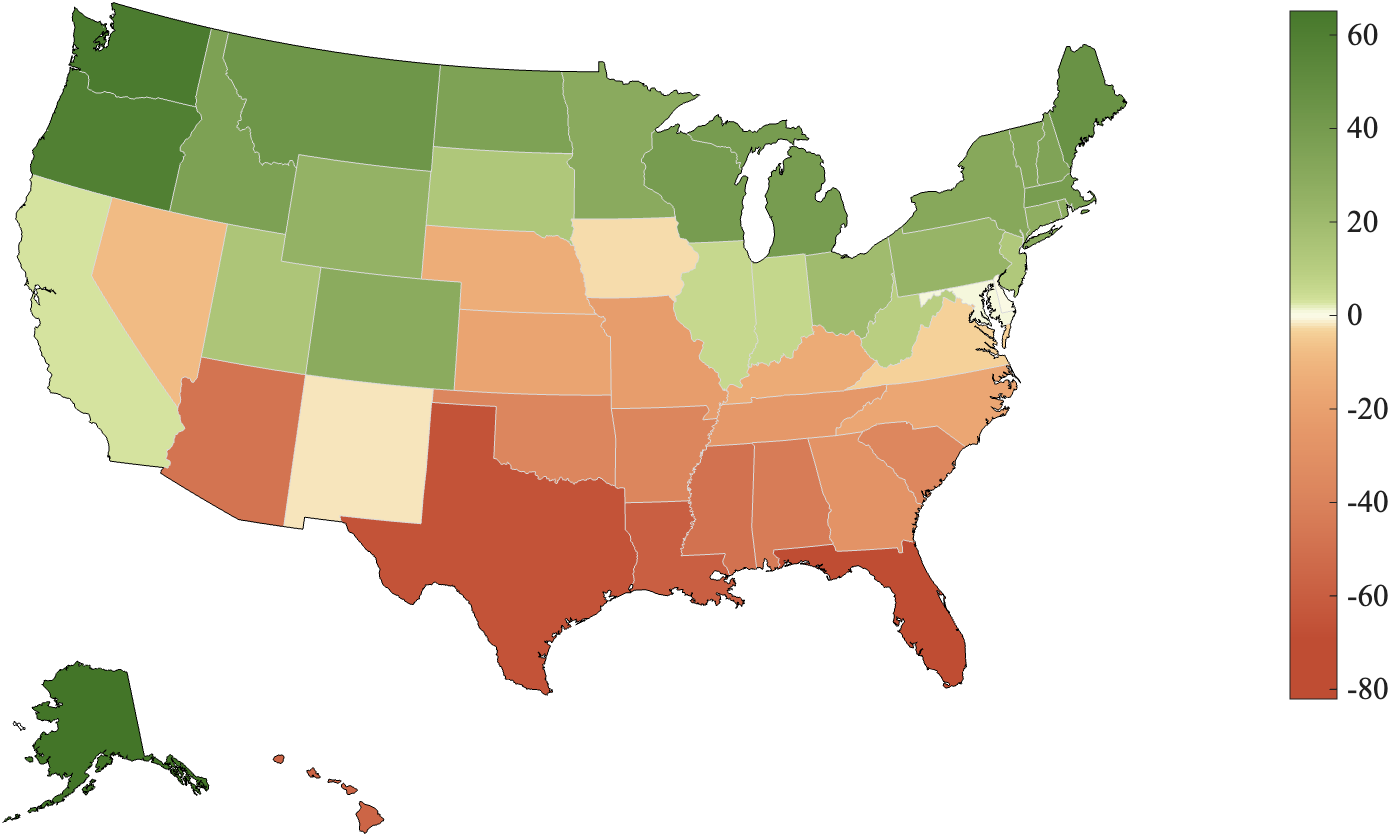
\includegraphics[height=0.43\textheight]{../Output/big_nu/graph_perfect_foresight/transition_maps/transition_maps_local_pop_changes_pct.png}
            \begin{itemize}\scriptsize\setlength{\itemsep}{1pt}
                \item \textbf{South empties:} Florida loses $>80\%$ of population; Southeast drops $20\text{--}30\%$.
                \item \textbf{North expands:} Alaska, Maine, Pacific NW gain $+20\text{--}60\%$.
            \end{itemize}
        \end{column}
        \begin{column}{0.48\textwidth}
            \centering
            \textbf{\small Wealth-to-Income Ratio Change ($\Delta (W/Y)_\ell$)}\\
            \vspace{0.04cm}
            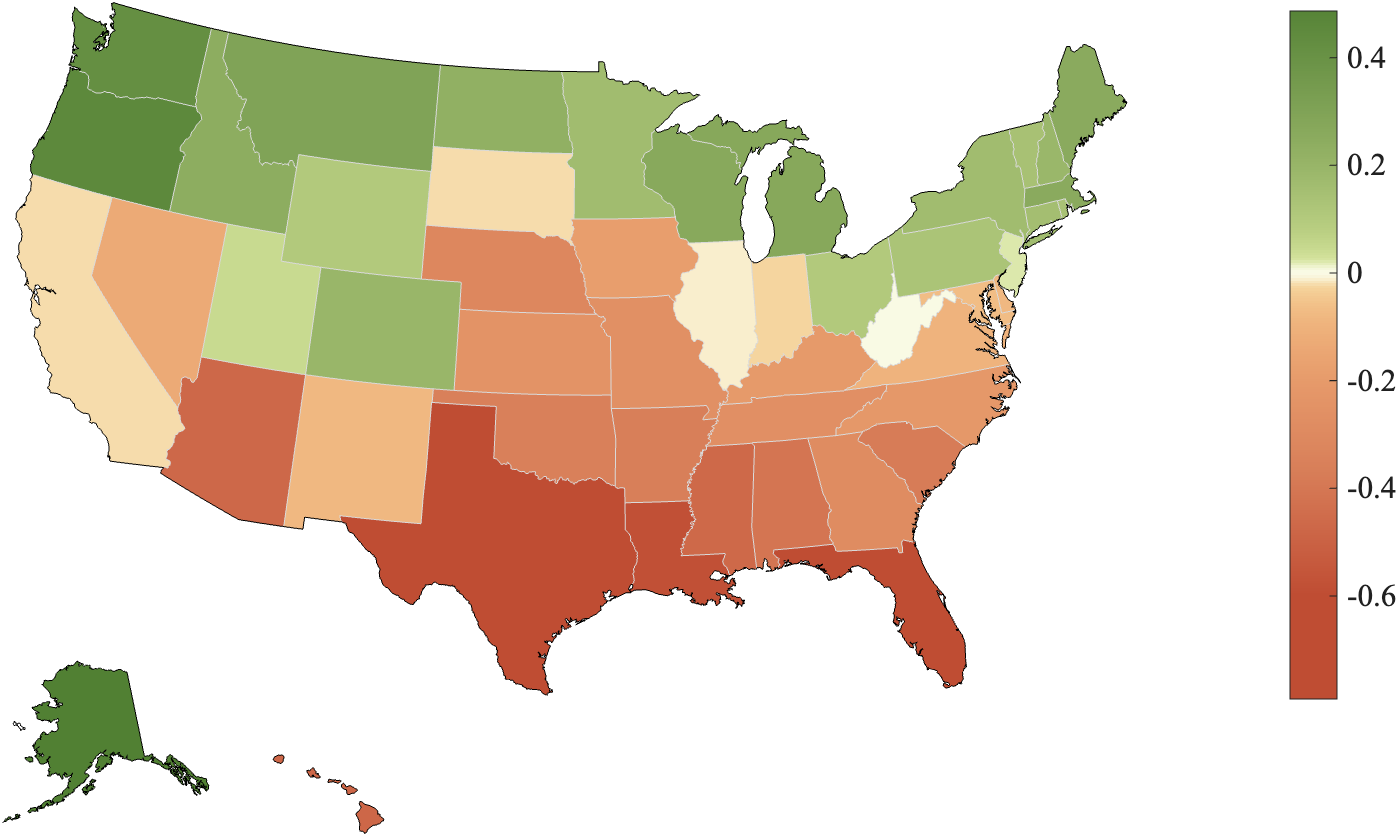
\includegraphics[height=0.43\textheight]{../Output/big_nu/graph_perfect_foresight/transition_maps/transition_maps_wealth_income_ratio_changes.png}
            \begin{itemize}\scriptsize\setlength{\itemsep}{1pt}
                \item \textbf{Southern contraction:} Wealth drops $>20\%$ in FL and LA due to lost spatial option value.
                \item \textbf{Northern accumulation:} Wealth surges $>10\%$ in MT and OR to buffer future migration risk.
            \end{itemize}
        \end{column}
    \end{columns}
\end{frame}


\begin{frame}{5-Channel Spatial Wealth Change Decomposition}\label{backup:5channel_decomp}
    \begin{columns}[T]
        \begin{column}{0.54\textwidth}
            \centering
            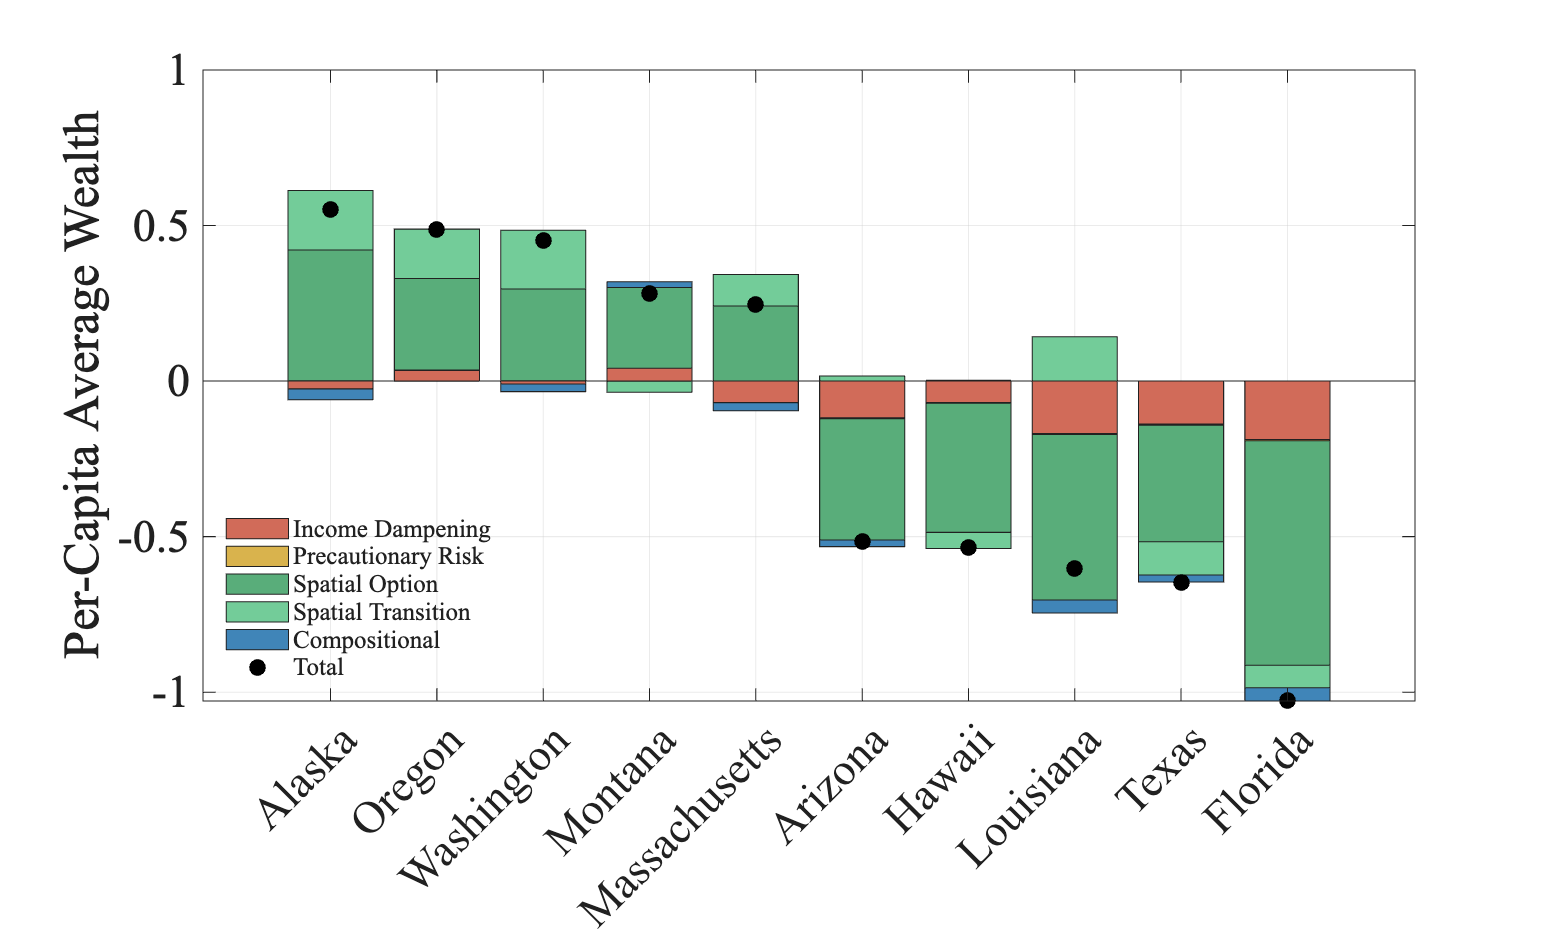
\includegraphics[width=\textwidth, height=0.72\textheight, keepaspectratio]{../Output/big_nu/graph_perfect_foresight/exact_percapita_decomposition_bar_no_counterfactual_no_counterfactual.png}
        \end{column}
        \begin{column}{0.44\textwidth}
            \begin{tcolorbox}[leafbox, title=Decomposition Insights]
                \scriptsize
                \begin{itemize}\setlength{\itemsep}{2pt}
                    \item \textbf{Damaged States (e.g., FL, MS):} Dominated by negative \textcolor{emerald}{Spatial Option Value} and negative \textcolor{terracotta}{Damage Dampening}.
                    \item \textbf{Haven States (e.g., MT, ME, OR):} Dominated by positive \textcolor{lightemerald}{Spatial Transition}  (inflow of historical wealth) and \textcolor{emerald}{Spatial Option Value}.
                    \item \textcolor{cobaltblue}{Compositional Sorting:} Mildly negative in damagedststates as high-productivity workers selectively concentrate.
                    \item \textcolor{mutedgold}{Precautionary Risk:} Creates almost no effect.
                \end{itemize}
            \end{tcolorbox}
        \end{column}
    \end{columns}
\end{frame}

% SLIDE 17: MYOPIA COUNTERFACTUAL
\begin{frame}{The Importance of Anticipation: Myopia Counterfactual \hfill \hyperlink{backup:myopia_dynamics}{\scriptsize\beamergotobutton{Myopia Audit}}}\label{main:myopia}
    \begin{columns}[T]
        \begin{column}{0.44\textwidth}
            \begin{tcolorbox}[leafbox, title=Mechanism: Myopia vs. Foresight]
                \scriptsize
                \begin{itemize}\setlength{\itemsep}{1pt}
                    \item \textbf{Myopic expectations:} Agents assume current fundamentals persist forever; no backward induction.
                    \item \textbf{No Precautionary Saving:} Instead of accumulating wealth ($+4.5\%$), myopic wealth \textit{falls} as shocks hit unexpectedly.
                    \item \textbf{Welfare Penalty:} Welfare loss in 2100 is $4\times$ larger under myopia ($-0.8\%$ vs $-0.2\%$).
                    \item \textbf{Delayed Convergence:} Takes 400 years vs 300 years to reach the terminal steady state.
                \end{itemize}
            \end{tcolorbox}
        \end{column}
        \begin{column}{0.54\textwidth}
            \centering
            \textbf{\scriptsize Aggregate Wealth ($W_t$ [Normalized]) under Myopia}\\
            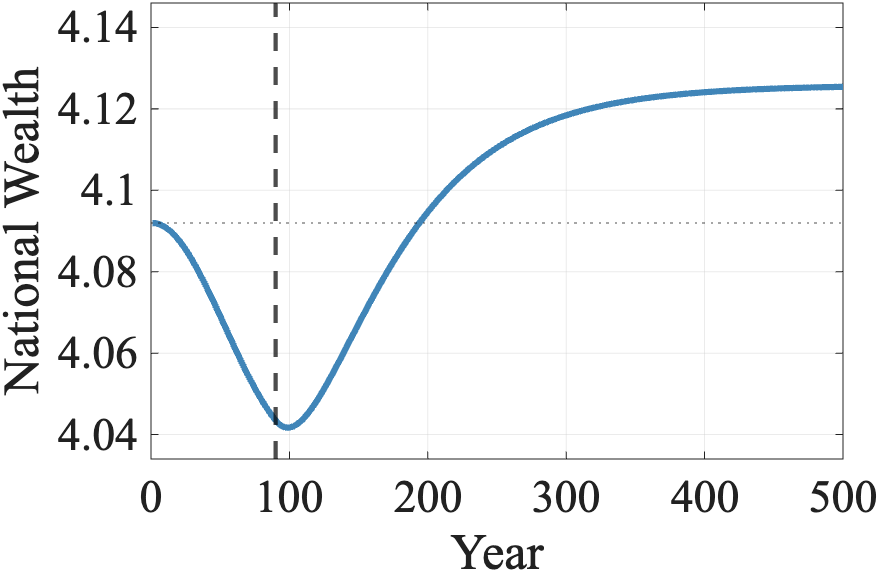
\includegraphics[height=0.34\textheight]{../Output/big_nu/graph_myopia/dynamic_moments/dynamic_moments_national_wealth.png}\\
            \vspace{0.04cm}
            \textbf{\scriptsize Wealth-to-Income Ratio ($(W/Y)_t$) under Myopia}\\
            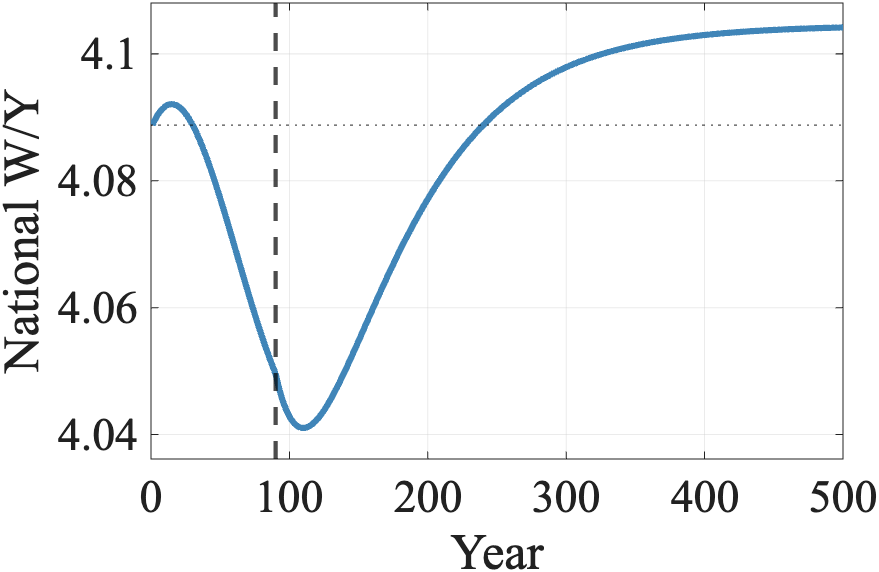
\includegraphics[height=0.34\textheight]{../Output/big_nu/graph_myopia/dynamic_moments/dynamic_moments_national_wy.png}
        \end{column}
    \end{columns}
\end{frame}

% SLIDE 18: COUNTERFACTUALS (NO MIGRATION VS NO SAVING)
\begin{frame}{Evaluating Adaptive Margins: Autarky vs. Hand-to-Mouth \hfill \hyperlink{backup:nomig_did}{\scriptsize\beamergotobutton{Autarky DiD}} \hyperlink{backup:nosaving_struct}{\scriptsize\beamergotobutton{No Saving}}}\label{main:margins}
    \begin{columns}[T]
        \begin{column}{0.485\textwidth}
            \textbf{\small Counterfactual 1: No Migration ($\psi_{j\ell} = 10^8$)}
            \begin{itemize}\scriptsize\setlength{\itemsep}{1pt}
                \item \textbf{Substitutability:} Workers cannot move $\to$ rely exclusively on financial savings.
                \item Peak W/Y ratio surges to \textbf{$+6.0\%$} (vs $+4.5\%$ baseline).
                \item \textbf{Flat Wealth Map:} Spatial wealth distribution becomes completely uniform.
                \item \textbf{Welfare Loss:} \textbf{$-1.5\%$} ($3\times$ baseline loss).
            \end{itemize}
            \vspace{0.04cm}
            \centering
            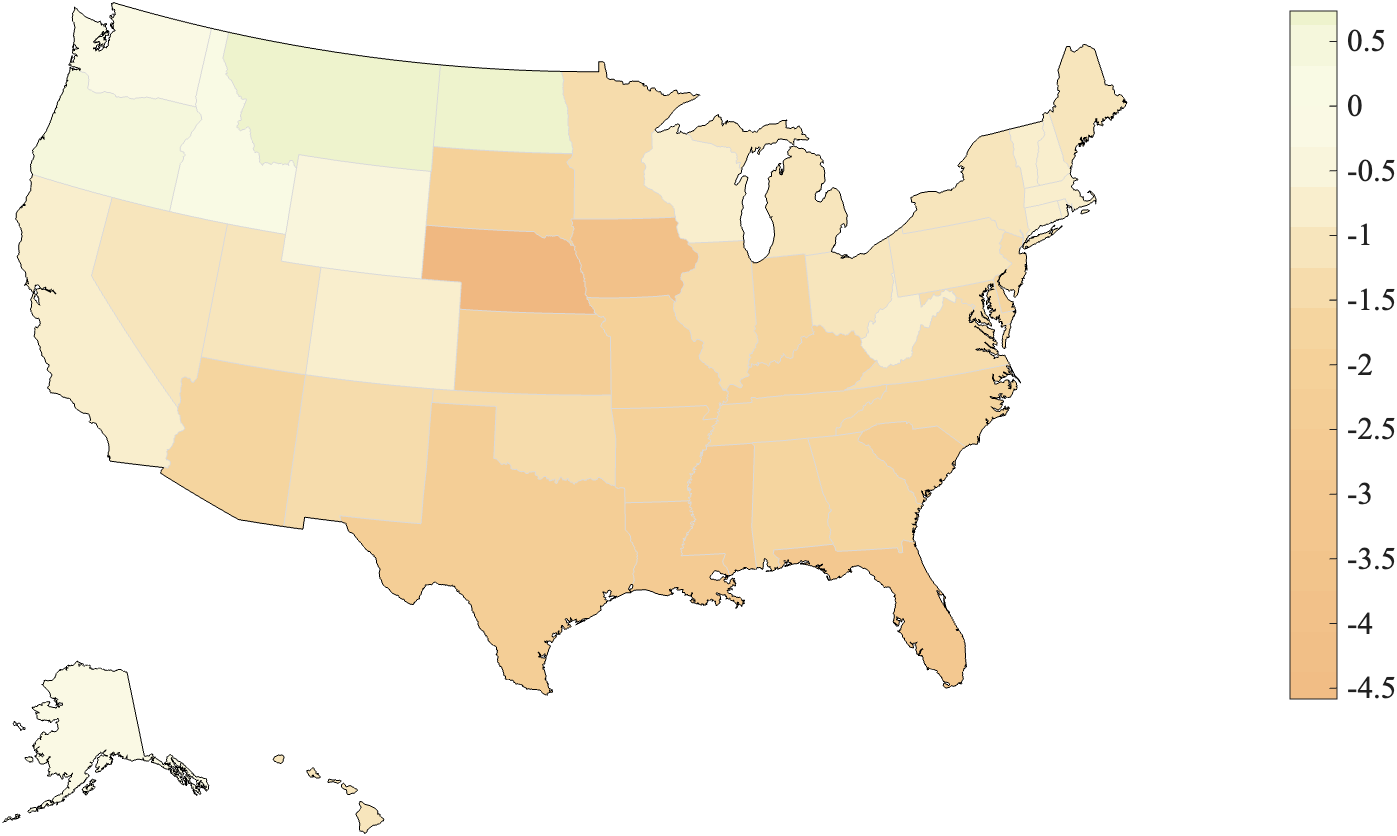
\includegraphics[width=\textwidth, height=0.36\textheight, keepaspectratio]{../Output/big_nu/graph_no_migration_did/transition_maps/transition_maps_pop_changes_pp.png}\\
            \vspace{0.02cm}
            {\scriptsize \textbf{Wealth Change (\%)under Autarky}}
        \end{column}
        \begin{column}{0.485\textwidth}
            \textbf{\small Counterfactual 2: No Saving ($a \equiv 0$)}
            \begin{itemize}\scriptsize\setlength{\itemsep}{1pt}
                \item \textbf{Substitutability:} Mobility rate rises from $2.5\%$ to $2.75\%$ to smooth shocks.
                \item \textbf{Variance Barrier:} High-wage North imposes higher uninsurable risk $\frac{1}{2}(\gamma \tilde{w}_\ell)^2 \sigma_\eta^2$; migrants get trapped.
                \item \textbf{Welfare Loss:} \textbf{$-2.8\%$} ($5.6\times$ baseline loss).
            \end{itemize}
            \vspace{0.04cm}
            \centering
            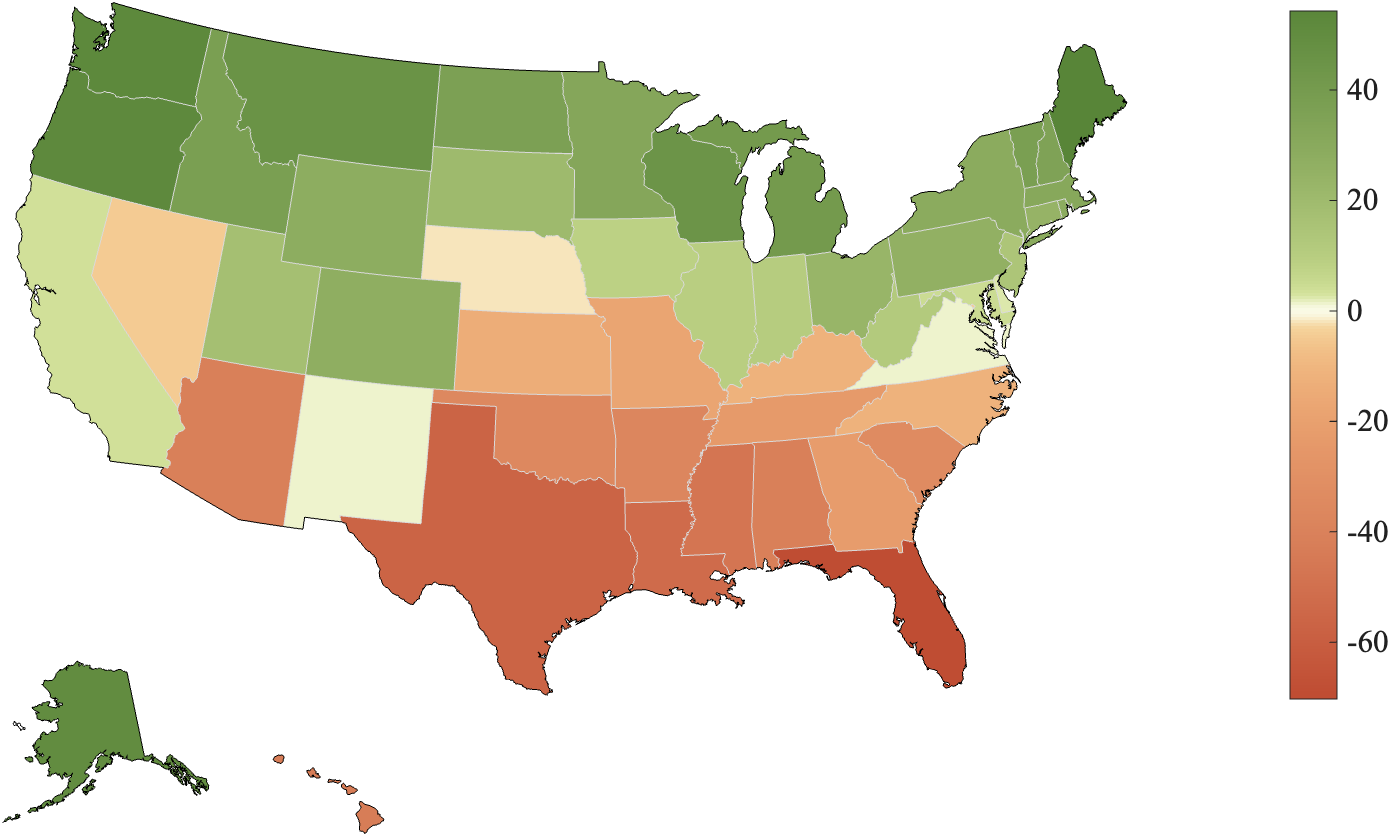
\includegraphics[width=\textwidth, height=0.36\textheight, keepaspectratio]{../Output/big_nu/graph_no_saving_struct/transition_maps/transition_maps_local_pop_changes_pct.png}\\
            \vspace{0.02cm}
            {\scriptsize \textbf{Local Population Change (\%) under Hand-to-Mouth}}
        \end{column}
    \end{columns}
\end{frame}

% SLIDE 19: COMPARISON & CROSS-SCENARIO SYNTHESIS
\begin{frame}{Cross-Scenario Synthesis: Substitutes, Complements, and Welfare \hfill \hyperlink{backup:welfare_metric}{\scriptsize\beamergotobutton{CE Derivation}}}\label{main:synthesis}
    \begin{columns}[onlytextwidth, T]
        \begin{column}{0.485\textwidth}
            \centering
            \textbf{\scriptsize Aggregate Welfare Loss (\% of Baseline Cons.)}\\
            \vspace{0.01cm}
            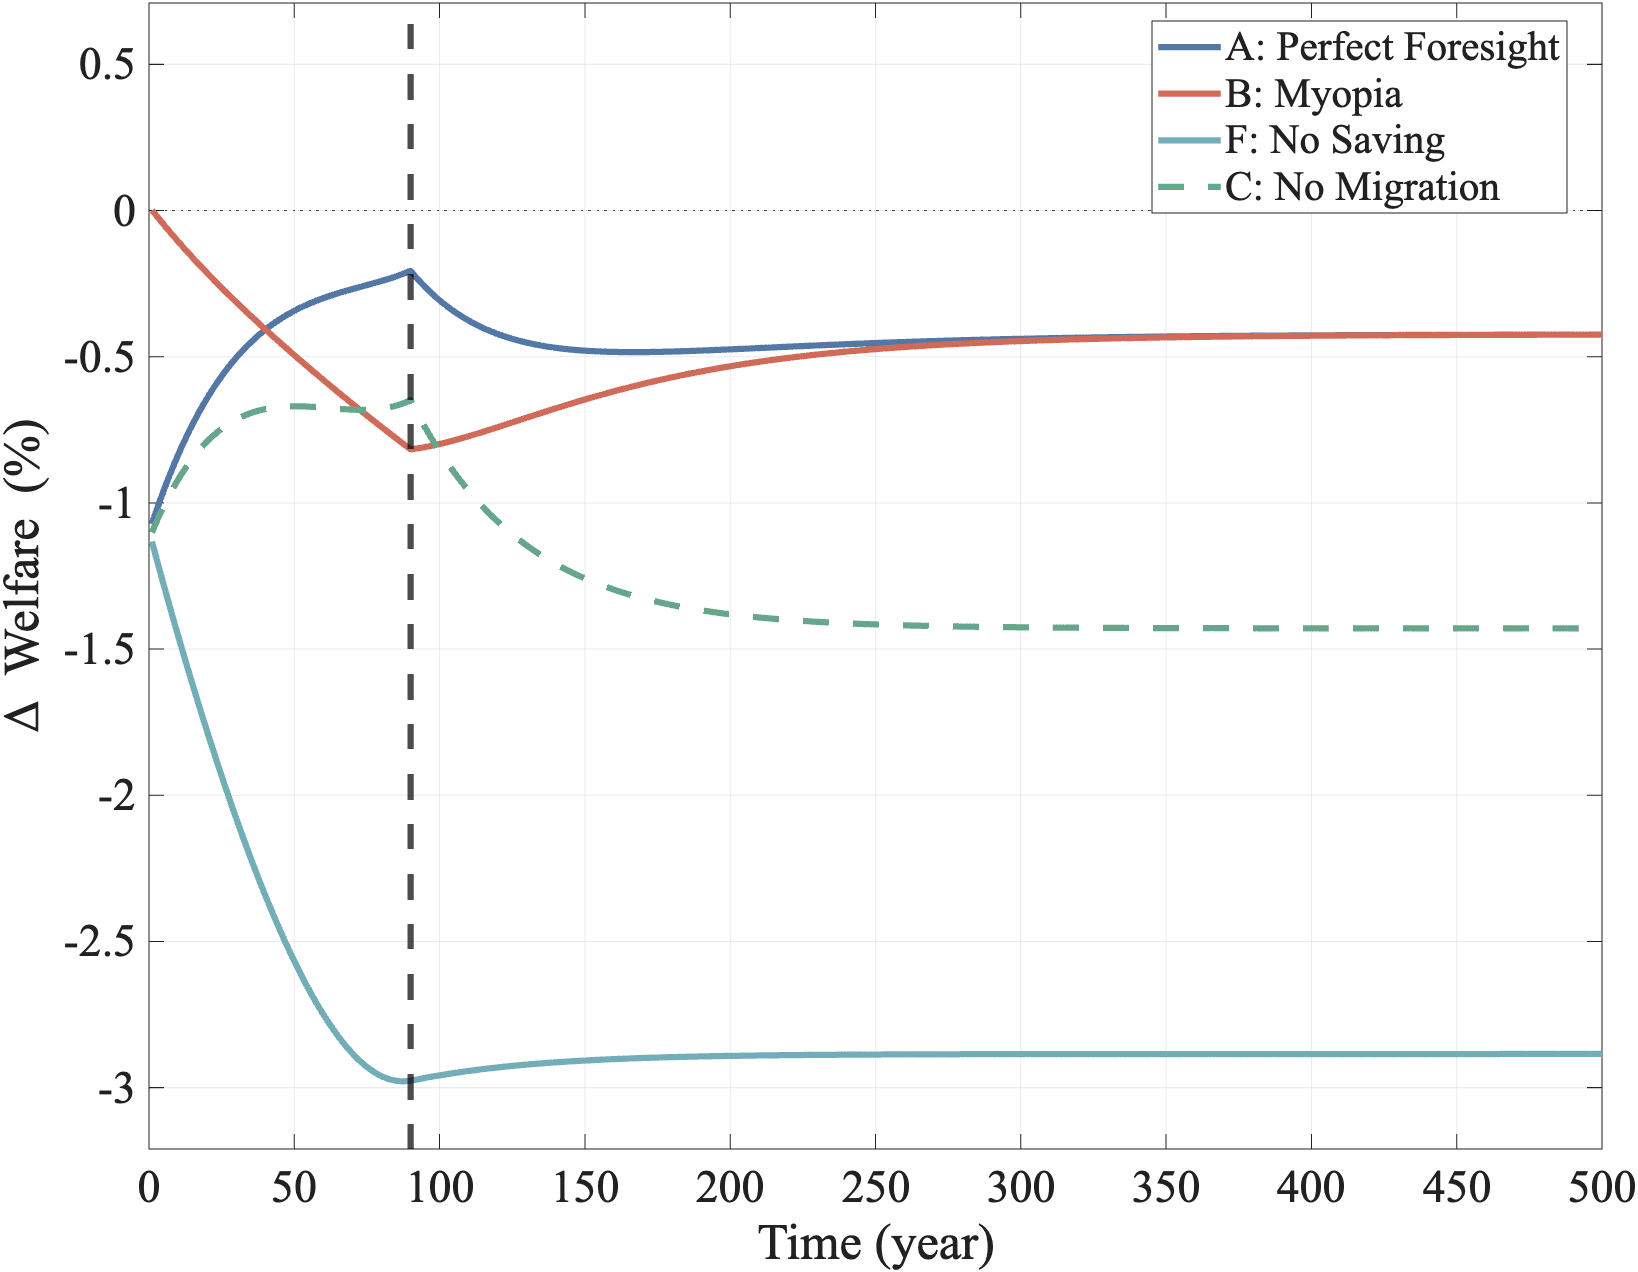
\includegraphics[width=\textwidth, height=0.50\textheight, keepaspectratio]{../Output/big_nu/graph_welfare_audit/welfare_audit_all_scenarios_ce_pct_frictions.png}\\
            \vspace{0.02cm}
            \scriptsize
            \setlength{\tabcolsep}{2.0pt}
            \renewcommand{\arraystretch}{0.88}
            \begin{tabular}{lcccc}
                \toprule
                \textbf{Scenario} & \textbf{Foresight} & \textbf{Save} & \textbf{Move} & \textbf{Term. $\Delta\text{CE}$} \\
                \midrule
                \textbf{Baseline} & \checkmark & \checkmark & \checkmark & \textbf{$-0.50\%$} \\
                \textbf{Myopia} & $\times$ & \checkmark & \checkmark & $-0.50\%$ \tiny($4\times$ in 2100) \\
                \textbf{No Migration} & \checkmark & \checkmark & $\times$ & \textbf{$-1.50\%$} \\
                \textbf{No Saving} & \checkmark & $\times$ & \checkmark & \textbf{$-2.80\%$} \\
                \bottomrule
            \end{tabular}
        \end{column}
        \begin{column}{0.485\textwidth}
            \centering
            \textbf{\scriptsize Wealth-to-Earnings Ratio Transition ($\Delta(W/Y)_t$ [\%])}\\
            \vspace{0.01cm}
            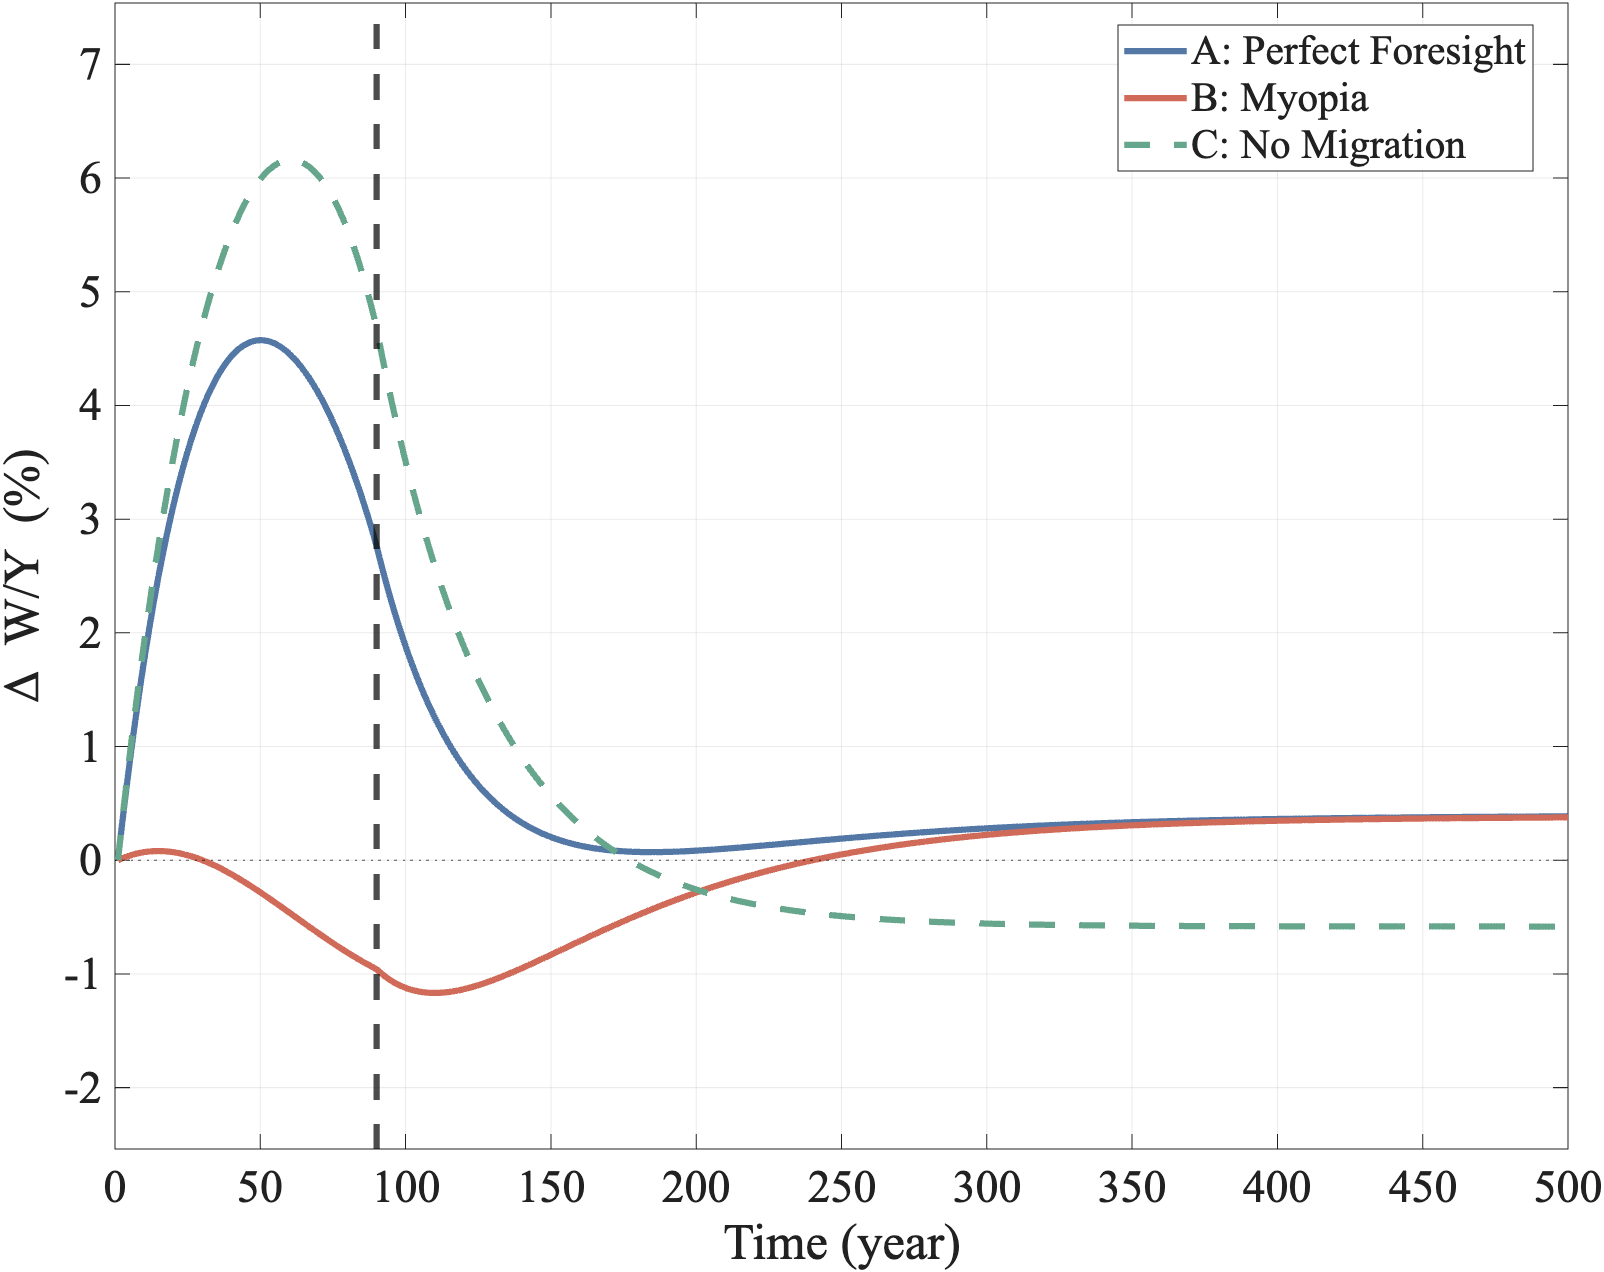
\includegraphics[width=\textwidth, height=0.50\textheight, keepaspectratio]{../Output/big_nu/graph_macro_audit/macro_wy_frictions/macro_wy_frictions_macro_wy_delta_wy_pct.png}\\
            \tiny
                \begin{itemize}\setlength{\itemsep}{0.5pt}
                    \item \textbf{Substitutes:} Closing one margin inflates reliance on the other ($W/Y \uparrow +6\%$ without mobility; $m_t \uparrow 2.75\%$ without saving).
                    \item \textbf{Complements:} Savings enable workers to bear uninsurable income variance when sorting into high-wage states.
                \end{itemize}
      
        \end{column}
    \end{columns}
\end{frame}

% =========================================================================
% SECTION 6: CONCLUSION (SLIDE 20)
% =========================================================================
\section{Conclusion}

% SLIDE 20: CONCLUSION & LIMITATIONS
\begin{frame}{Conclusion \& Research Limitations \hfill \hyperlink{backup:toc}{\scriptsize\beamergotobutton{Appendix TOC}}}\label{main:conclusion}
    \begin{columns}[onlytextwidth, T]
        \begin{column}{0.49\textwidth}
            \textbf{Summary of Contributions:}
            \begin{itemize}\footnotesize\setlength{\itemsep}{2pt}
                \item \textbf{Methodology:} Overcome the curse of dimensionality with CARA preferences. Introduce dynamic transition, climate change, distinction between amenities and migration costs, and a 5-channel decomposition of spatial wealth change.
                \item \textbf{Quantitative Findings:} Aggregate US climate damages remain moderate ($-0.5\%$ welfare loss) due to joint adaptation, but with massive spatial reshaping (Florida loses $>80\%$ population, Northern wealth rises $>10\%$).
                \item \textbf{Adaptive Margins:} Demonstrates that saving and migration act simultaneously as substitutes and complements.
            \end{itemize}
        \end{column}
        \begin{column}{0.49\textwidth}
            \begin{tcolorbox}[leafbox, title=Structural Limitations \& Future Research]
                \scriptsize
                \begin{itemize}\setlength{\itemsep}{2pt}
                    \item \textbf{CARA Utility \& Credit Markets:} Constant absolute risk aversion abstracts from wealth effects on moving, precluding analysis of spatial poverty traps where low-wealth households cannot afford relocation.
                    \item \textbf{Partial Equilibrium Endowment Economy:} Fixed world interest rate $r = 0.03$; abstracts from general equilibrium capital accumulation, asset price declines, and direct climate destruction of physical capital.
                    \item \textbf{Local Agglomeration \& Dispersion Forces:} Does not model endogenous congestion in housing markets or labor agglomeration spillovers in receiving Northern states.
                \end{itemize}
            \end{tcolorbox}
        \end{column}
    \end{columns}
\end{frame}
\begin{frame}
  \Large \centering \textbf{Thank you for your attention!}
\end{frame}
% =========================================================================
% APPENDIX / BACKUP SLIDES (>= 20 BACKUP SLIDES ACROSS ALL SECTIONS)
% =========================================================================
\appendix

% -------------------------------------------------------------------------
% APPENDIX TABLE OF CONTENTS
% -------------------------------------------------------------------------
% -------------------------------------------------------------------------
% APPENDIX SECTION 1: INTRODUCTION, LITERATURE & DATA SOURCES
% -------------------------------------------------------------------------
\section{Appendix: Introduction \& Data Sources}

\begin{frame}{Appendix: Literature Taxonomy on Dynamic Spatial Macro Models \hfill \hyperlink{main:fact3}{\scriptsize\beamerreturnbutton{Return}}}\label{backup:lit_taxonomy}
    \centering
    \tiny
    \renewcommand{\arraystretch}{0.95}
    \begin{tabularx}{\textwidth}{lccccX}
        \toprule
        \textbf{Model / Paper} & \textbf{\shortstack{Forward\\Migration}} & \textbf{\shortstack{Worker\\Savings}} & \textbf{\shortstack{Transition\\Dynamics}} & \textbf{\shortstack{Climate\\Damages}} & \textbf{Methodology / Mechanism} \\
        \midrule
        Desmet et al. (2018) & No & No & Yes & Yes & Static location choice sequential equilibrium \\
        Caliendo et al. (2019) & Yes & No & Yes & No & Hand-to-mouth workers, trade \& spatial dynamics \\
        Kleinman et al. (2023) & Yes & Capitalists & Yes & No & Mobile hand-to-mouth + immobile capitalists \\
        Bilal et al. (2026) & Yes & Capitalists & Yes & Yes & Same as Kleiman (2023) with the Master Equation \\
        Sun (2025) & Yes & Yes & Yes & Yes & Deep learning value function approximation \\
        Giannone et al. (2023) & Yes & Yes & Yes & No & Overlapping generations (OLG) framework \\
        Donald et al. (2025) & Yes & Yes & Yes & No & Sequence-space Jacobian (small aggregate shocks) \\
        Dvorkin \& Greaney (2025) & Yes & Yes & \textbf{No} & \textbf{No} & CARA closed-form, static steady states \\
        \midrule
        \textbf{This Thesis (2026)} & \textbf{Yes} & \textbf{Yes} & \textbf{Yes} & \textbf{Yes} & \textbf{CARA closed-form, 500-yr transition path, empirical 6-sector climate damage mapping} \\
        \bottomrule
    \end{tabularx}
    \vspace{0.04cm}
    \begin{tcolorbox}[takeawaybox]
        \scriptsize This thesis bridges the gap between high-dimensional dynamic spatial models and analytical tractability, enabling decompositions of savings and migration margins during climate transitions.
    \end{tcolorbox}
\end{frame}

\begin{frame}{Appendix: Empirical Climate Facts \& The Paris Agreement Gap \hfill \hyperlink{main:fact1}{\scriptsize\beamerreturnbutton{Return}}}\label{backup:climate_facts}
    \begin{columns}[T]
        \begin{column}{0.48\textwidth}
            \textbf{\small IPCC AR6 Projections (IPCC, 2023)}
            \vspace{0.05cm}
            \begin{itemize}\scriptsize\setlength{\itemsep}{2pt}
                \item \textbf{Historical Warming:} $+1.1^\circ\text{C}$ (2011--2020 relative to 1850--1900).
                \item \textbf{SSP1-2.6:} Low emissions, $+1.8^\circ\text{C}$ by 2100 (requires rapid net-zero CO$_2$).
                \item \textbf{SSP2-4.5:} Intermediate path, $+2.7^\circ\text{C}$ by 2100.
                \item \textbf{SSP5-8.5:} High emissions baseline, $+4.4^\circ\text{C}$ by 2100 (basis for Hsiang et al. 2017).
                \item Current policies track closest to \textbf{SSP2-4.5 / SSP3-7.0}, exceeding Paris $1.5^\circ\text{C}$ thresholds.
            \end{itemize}
        \end{column}
        
        \begin{column}{0.48\textwidth}
            \textbf{\small Paris Commitments vs. Reality}
            \vspace{0.05cm}
            \begin{itemize}\scriptsize\setlength{\itemsep}{2pt}
                \item \textbf{Target:} Limit warming to well below $2.0^\circ\text{C}$, pursuing $1.5^\circ\text{C}$.
                \item \textbf{Implementation Gap:} Nationally Determined Contributions imply an emissions gap of $15\text{--}20\text{ GtCO}_2\text{e}$ by 2030 (Barrage \& Nordhaus, 2023).
                \item \textbf{Frequency of Extremes:} 1-in-50 year extreme heat events now occur $4.8\times$ more frequently.
                \item \textbf{US Wildfires:} Western US burned forest area has increased by $>400\%$ since 1984.
            \end{itemize}
        \end{column}
    \end{columns}
\end{frame}

\begin{frame}{Appendix: Spatial Heterogeneity \& Hsiang et al. (2017) Methodology \hfill \hyperlink{main:fact2}{\scriptsize\beamerreturnbutton{Return}}}\label{backup:hsiang_method}
    \begin{columns}[T]
        \begin{column}{0.50\textwidth}
            \textbf{\small Econometric Framework (Hsiang et al., 2017)}
            \vspace{0.05cm}
            \begin{itemize}\scriptsize\setlength{\itemsep}{2pt}
                \item \textbf{Resolution:} 3,143 contiguous US counties.
                \item \textbf{Climate Models:} 40 global climate models (GCMs) downscaled to county grids under RCP 8.5.
                \item \textbf{Sectors Quantified (6 Channels):} (1)~Agriculture (crop yields), (2)~Mortality (heat deaths), (3)~Energy (electricity), (4)~Labor productivity, (5)~Crime (violent/property), (6)~Coastal storm damage \& SLR.
            \end{itemize}
        \end{column}
        
        \begin{column}{0.48\textwidth}
            \textbf{\small Aggregation \& Spatial Concentration}
            \vspace{0.05cm}
            \begin{itemize}\scriptsize\setlength{\itemsep}{2pt}
                \item County estimates aggregated to 51 states using income and population weights.
                \item \textbf{Steep Gradient:} Southern counties experience median damages $>10\%$ GDP, with tails reaching $28\%$.
                \item Northern counties benefit from reduced winter mortality and lower heating costs (net $+2\text{ to }+5\%$ GDP).
                \item Generates strong spatial incentives for labor and capital reallocation.
            \end{itemize}
        \end{column}
    \end{columns}
\end{frame}

\begin{frame}{Appendix: Spatial Mobility Frictions \& U.S. Migration Trends \hfill \hyperlink{main:environment}{\scriptsize\beamerreturnbutton{Return}}}\label{backup:migration_frictions}
    \begin{columns}[T]
        \begin{column}{0.48\textwidth}
            \textbf{\small Empirical U.S. Internal Migration Facts}
            \vspace{0.05cm}
            \begin{itemize}\scriptsize\setlength{\itemsep}{2pt}
                \item \textbf{Secular Decline in Mobility:} Inter-state migration rate has declined from $\sim 3.0\%$ in the 1980s to $\sim 1.5\text{--}2.5\%$ today (Molloy et al., 2011).
                \item \textbf{IRS SOI Data (2015--2016):} Tracks 95--98\% of tax-filing units across state lines (used in calibration).
                \item \textbf{Distance Penalty:} Moving probability falls sharply with distance ($\psi_{\text{dist}} = 0.405$).
                \item \textbf{Fixed Costs:} Large non-pecuniary relocation friction ($\psi_{\text{fix}} = 1.633$).
            \end{itemize}
        \end{column}
        
        \begin{column}{0.48\textwidth}
            \textbf{\small Idiosyncratic Preference Shocks ($\nu$)}
            \vspace{0.05cm}
            \begin{itemize}\scriptsize\setlength{\itemsep}{2pt}
                \item Weibull shape parameter $\nu = 3.95$ governs migration elasticity to wage/amenity gaps.
                \item Lower $\nu$ implies higher dispersion in idiosyncratic preferences, acting as non-monetary attachment to locations.
                \item \textbf{Sluggish Adaptation:} Because of these frictions, the full spatial reallocation takes $\sim 300$ years to converge.
            \end{itemize}
        \end{column}
    \end{columns}
\end{frame}

\begin{frame}{Appendix: Theoretical Foundations: Precautionary Savings vs. Mobility \hfill \hyperlink{main:saving_option}{\scriptsize\beamerreturnbutton{Return}}}\label{backup:theory_foundations}
    \begin{itemize}\small\setlength{\itemsep}{3pt}
        \item \textbf{Taxonomy of Adaptation Margins (Ehrlich \& Becker, 1972):}
        \begin{itemize}\footnotesize
            \item \textit{Self-Insurance (Saving):} Reduces the \textbf{severity} of consumption loss given an adverse state.
            \item \textit{Self-Protection (Migration):} Reduces the \textbf{probability} of remaining in an adverse economic state.
        \end{itemize}
        \item \textbf{CARA Incomplete Markets (Caballero, 1990):}
        \begin{equation}
            c_{\ell,t}(a, z^\prime, \eta^\prime) = \Xi_{\ell,t}(z^\prime) + \tfrac{r}{1+r}\left[\tilde{y}_{\ell,t} + \tilde{w}_{\ell,t}\eta^\prime + a\right]
        \end{equation}
        \begin{itemize}\footnotesize
            \item Constant absolute risk aversion ($\gamma = 3$) eliminates wealth effects on migration, allowing state-space reduction from $(a, z, \ell)$ to $(z, \ell)$.
        \end{itemize}
        \item \textbf{Location as an Asset (Bilal \& Rossi-Hansberg, 2021):}
        \begin{itemize}\footnotesize
            \item Moving to a high-amenity/high-wage location is an investment; borrowing constraints force low-wealth workers to substitute towards cheaper locations.
        \end{itemize}
    \end{itemize}
\end{frame}

\begin{frame}{Appendix: Comparison with Spatial Climate Models (S-IAMs) \hfill \hyperlink{main:contributions}{\scriptsize\beamerreturnbutton{Return}}}\label{backup:siam_comparison}
    \begin{columns}[T]
        \begin{column}{0.48\textwidth}
            \textbf{\small Existing S-IAM Estimates}
            \vspace{0.05cm}
            \begin{itemize}\scriptsize\setlength{\itemsep}{2pt}
                \item \textbf{Desmet \& Rossi-Hansberg (2024):} Global model with trade and migration, but abstracts from capital accumulation.
                \item \textbf{Krusell \& Smith (2022):} Dynamic capital accumulation across space, but assumes \textit{zero migration}.
                \item \textbf{Bilal \& Rossi-Hansberg (2026):} Mobile hand-to-mouth workers vs. immobile capitalists ($1.1\%$ to $4.6\%$ global welfare loss, with also important heterogeneity).
                \item \textbf{Hsiang et al. (2017):} Econometric reduced-form, zero endogenous adaptation ($6\%$ US GDP loss).
            \end{itemize}
        \end{column}
        
        \begin{column}{0.48\textwidth}
            \textbf{\small Why our Baseline Welfare Loss is 0.5\%}
            \vspace{0.05cm}
            \begin{itemize}\scriptsize\setlength{\itemsep}{2pt}
                \item \textbf{Joint Adaptation Margin:} Enabling \textit{both} forward-looking precautionary saving and spatial reallocation cushions the shock.
                \item In our \textbf{No-Saving counterfactual}, welfare loss jumps to \textbf{2.8\%} (matching hand-to-mouth models).
                \item In our \textbf{No-Migration counterfactual}, welfare loss triples to \textbf{1.5\%}.
                \item \textbf{Takeaway:} Omitting adaptation margins biases estimated climate damage costs upwards.
            \end{itemize}
        \end{column}
    \end{columns}
\end{frame}

% SLIDE A: EMPIRICAL DATA SOURCES MAPPING (R4)
\begin{frame}{Appendix: Empirical Data Sources \& Model Parameter Mapping \hfill \hyperlink{main:calibration}{\scriptsize\beamerreturnbutton{Return}}}\label{backup:data_sources}
    \begin{columns}[T]
        \begin{column}{0.48\textwidth}
            \textbf{\small Microdata \& Administrative Records}
            \vspace{0.04cm}
            \begin{itemize}\scriptsize\setlength{\itemsep}{2pt}
                \item \textbf{IRS SOI Migration (2015--2016):}
                \begin{itemize}\tiny
                    \item Administrative bilateral tax-filer flows between all 51 states.
                    \item \textit{Target:} Gross mobility ($2.50\%$) \& log-distance ($0.5032$) $\to$ identifies moving costs $(\psi_{\text{fix}} = 1.633, \psi_{\text{dist}} = 0.405)$.
                \end{itemize}
                \item \textbf{CPS-ORG Microdata (2010--2015):}
                \begin{itemize}\tiny
                    \item Prime-age earnings (25--60) trimmed at $1\%/99\%$.
                    \item \textit{Output:} National mean income $\bar{Y}_{\text{US}} = \$48,669$ (model numeraire) \& state base wages $\{w_\ell\}$.
                \end{itemize}
                \item \textbf{PSID Wage Panel (1991--1997):}
                \begin{itemize}\tiny
                    \item Autocovariance ratio of wage residuals $\to$ persistence $\rho = 0.934$.
                \end{itemize}
                \item \textbf{SCF \& Geowealth-US (Suss \& Greaney 2024):}
                \begin{itemize}\tiny
                    \item Aggregate $W/Y = 4.089 \to$ identifies preference scale $\bar{\lambda} = 0.371$; validates state wealth out-of-sample ($r=0.68$).
                \end{itemize}
            \end{itemize}
        \end{column}
        
        \begin{column}{0.50\textwidth}
            \textbf{\small National Accounts \& Regional Fundamentals}
            \vspace{0.04cm}
            \begin{itemize}\scriptsize\setlength{\itemsep}{2pt}
                \item \textbf{BEA SAGDP2 (GDP by State):}
                \begin{itemize}\tiny
                    \item Agricultural GDP share $s_\ell^{\text{agri}} = \text{Agri\_GDP}_\ell/\text{Total\_GDP}_\ell$ ($2010\text{--}2015$ avg).
                \end{itemize}
                \item \textbf{BEA RPP \& BLS Consumer Expenditure Survey:}
                \begin{itemize}\tiny
                    \item Housing cost $q_\ell = \alpha_h (\text{RPP}_\ell / 100)$ with $\alpha_h = 0.30$.
                    \item Residential electricity expenditure share $s_\ell^{\text{energy}}$.
                \end{itemize}
                \item \textbf{US Decennial Census \& ACS (2015):}
                \begin{itemize}\tiny
                    \item State population shares $\tilde{p}_\ell \to$ BLP contraction mapping recovers baseline amenities $\{A_\ell\}$.
                \end{itemize}
                \item \textbf{Amenity Validation Regressors:}
                \begin{itemize}\tiny
                    \item USDA Natural Amenities, NAEP Math/Reading (NCES), Fraser Institute EFNA, FBI UCR Crime, Census CBP variety.
                \end{itemize}
            \end{itemize}
        \end{column}
    \end{columns}
    \vspace{0.05cm}
    \begin{tcolorbox}[takeawaybox]
        \scriptsize \textbf{Empirical Grounding:} All 51 state economies are anchored in administrative microdata and national accounts, separating moving frictions from baseline quality-of-life amenities.
    \end{tcolorbox}
\end{frame}

% SLIDE B: CLIMATE DAMAGE MAPPING EQUATIONS (R4)
\begin{frame}{Appendix: Climate Damage Mapping: County Projections to 3 Channels \hfill \hyperlink{main:damage_mapping}{\scriptsize\beamerreturnbutton{Return}}}\label{backup:damage_channels}
    \begin{columns}[T]
        \begin{column}{0.48\textwidth}
            \textbf{\small Hsiang et al. (2017) Damage Sectors}
            \vspace{0.04cm}
            \begin{itemize}\scriptsize\setlength{\itemsep}{2pt}
                \item \textbf{Labor Productivity ($\bar{L}_\ell$):} High- \& low-risk worker heat exposure $\to$ income-weighted.
                \item \textbf{Agricultural Yields ($\bar{Y}_\ell^{\text{agri}}$):} 4 major crops (corn, soy, wheat, cotton) $\to$ income-weighted.
                \item \textbf{Coastal Storm Damage ($\bar{C}_\ell$):} Surge \& inundation capital loss $\to$ income-weighted.
                \item \textbf{Mortality ($\bar{M}_\ell$):} Heat/cold death rate $\to$ pop-weighted.
                \item \textbf{Crime Rates ($\bar{R}_\ell$):} Violent \& property $\to$ pop-weighted.
                \item \textbf{Energy Costs ($\bar{E}_\ell$):} Electricity use $\to$ income-weighted.
            \end{itemize}
        \end{column}
        
        \begin{column}{0.50\textwidth}
            \textbf{\small Channel Mapping Equations}
            \vspace{0.04cm}
            \begin{itemize}\scriptsize\setlength{\itemsep}{2.5pt}
                \item \textbf{Wage Shock ($\Delta w_\ell$):}
                $$\Delta w_\ell = \frac{\bar{L}_\ell}{100} + \frac{\bar{Y}_\ell^{\text{agri}}}{100} s_\ell^{\text{agri}} - \frac{\bar{C}_\ell}{100}$$
                \item \textbf{Amenity Shock ($\Delta A_\ell$):}
                $$\Delta A_\ell = \gamma \left[ \frac{\bar{M}_\ell}{10^5} \frac{\text{VSL}}{\bar{Y}_{\text{US}}} + \frac{\bar{R}_\ell}{10^5} \frac{\mathbb{E}[\text{VSC}]}{\bar{Y}_{\text{US}}} \right]$$
                \item \textbf{Housing Cost Shock ($\Delta q_\ell$):}
                $$\Delta q_\ell = \frac{\bar{E}_\ell}{100} s_\ell^{\text{energy}}$$
            \end{itemize}
            \vspace{0.02cm}
            \begin{tcolorbox}[leafbox]
                \tiny \textbf{Monetization Anchor:} EPA $\text{VSL} = \$9.0\text{M}$; FBI/McCollister $\text{VSC}_{\text{viol}} = \$205.8\text{k}, \text{VSC}_{\text{prop}} = \$4.8\text{k}$; $\bar{Y}_{\text{US}} = \$48,669$.
            \end{tcolorbox}
        \end{column}
    \end{columns}
\end{frame}

% -------------------------------------------------------------------------
% APPENDIX SECTION 2: MODEL & THEORY BACKUP
% -------------------------------------------------------------------------
\section{Appendix: Model \& Theory}

\begin{frame}{Appendix: Derivation and Proof of Proposition 1 \hfill \hyperlink{main:prop1}{\scriptsize\beamerreturnbutton{Return}}}\label{backup:prop1_proof}
    \begin{itemize}\small\setlength{\itemsep}{2pt}
        \item \textbf{Euler Equation under CARA Utility:}
        Under $u(c, A) = -\frac{1}{\gamma}e^{-\gamma c - \tilde{A}}$, the first-order condition with respect to next-period assets $a'$ is:
        {\small
        $$e^{-\gamma c_{\ell,t}} = \beta (1+r) \mathbb{E}_t \left[ e^{-\gamma c_{m,t+1}} \right]$$
        }
        \item \textbf{Policy Guess \& Budget Substitution:}
        {\scriptsize
        \begin{align*}
        c_{\ell,t} &= \Xi_{\ell,t}(z^\prime) + \tfrac{r}{1+r}\left[\tilde{y}_{\ell,t} + \tilde{w}_{\ell,t}\eta^\prime + a\right] \\
        a_{\ell,t+1} &= \tilde{y}_{\ell,t} + \tilde{w}_{\ell,t}\eta^\prime + a + (1+r)(\tilde{w}_{\ell,t}z^\prime - \Xi_{\ell,t}(z^\prime))
        \end{align*}
        }
        \item \textbf{Transitory Shock Integration ($\eta^\prime \sim \mathcal{N}(0, \sigma_{\eta,\ell}^2)$):}
        {\small
        $$\mathbb{E}_{\eta^\prime} \left[ \exp\left(-\gamma \tfrac{r}{1+r} \tilde{w}_{\ell,t}\eta^\prime\right) \right] = \exp\left( \tfrac{1}{2}\left(\gamma \tfrac{r}{1+r}\tilde{w}_{\ell,t}\right)^2 \sigma_{\eta,\ell}^2 \right)$$
        }
        \item \textbf{Weibull Extreme Value Property:} For i.i.d. Weibull shocks $\varepsilon_m \sim \text{Weibull}(\nu, \lambda)$:
        {\small
        $$\mathbb{E}_\varepsilon \left[ \max_{m=1,\dots,J} \left\{ \varepsilon_m X_m \right\} \right] = \bar{\lambda} \left[ \tfrac{1}{J} \sum_{m=1}^J X_m^{-\nu} \right]^{-1/\nu}$$
        }
        Equating value functions yields the recursive contraction mapping for $\Xi_{\ell,t}(z^\prime)$ in Proposition 1.
    \end{itemize}
\end{frame}

% STREAMLINED SLIDE 28: EX-ANTE WEIBULL BELLMAN (R3)
\begin{frame}{Appendix: Ex-Ante Value Function \& Multiplicative Factorization \hfill \hyperlink{main:prop1}{\scriptsize\beamerreturnbutton{Return}}}\label{backup:exante_bellman}
    \begin{columns}[T]
        \begin{column}{0.48\textwidth}
            \textbf{\small Ex-Ante Weibull Choice Expectation}
            \vspace{0.04cm}
            \begin{itemize}\scriptsize\setlength{\itemsep}{2pt}
                \item \textbf{Discrete Choice over Destinations:}
                Workers choose destination location $\ell \in \{1,\dots,J\}$ facing idiosyncratic preference shocks $\varepsilon \sim \text{Weibull}(\nu, \lambda)$:
                $$V_{j,t}(a, z, \boldsymbol{\varepsilon}) = \max_{\ell \in \{1,\dots,J\}} \left\{ \varepsilon_\ell U_{j\ell,t}(a, z) \right\}$$
                \item \textbf{Closed-Form Weibull Ex-Ante Expectation:}
                Integrating over $\boldsymbol{\varepsilon}$ collapses the discrete choice into the power-mean:
                $$v_{j,t}(a, z) \equiv \mathbb{E}_{\boldsymbol{\varepsilon}} [V_{j,t}] = -\bar{\lambda} \left[ \frac{1}{J} \sum_{\ell=1}^J |U_{j\ell,t}(a, z)|^{-\nu} \right]^{-1/\nu}$$
                \item \textbf{Streamlined Dynamic Program:}
                Eliminates intermediate value function layers, characterizing the entire equilibrium via the single ex-ante value $v_{j,t}(a, z)$.
            \end{itemize}
        \end{column}
        
        \begin{column}{0.48\textwidth}
            \textbf{\small Multiplicative Wealth Factorization}
            \vspace{0.04cm}
            \begin{itemize}\scriptsize\setlength{\itemsep}{2pt}
                \item \textbf{Factorization Property:}
                $$v_{j,t}(a, z) = -\tfrac{1}{\gamma} \exp\left(-\gamma \tfrac{r}{1+r} a\right) \exp\left(-\gamma \Xi_{j,t}(z)\right)$$
                \item \textbf{Wealth Invariance of Migration:}
                Financial wealth $a$ factors out as an identical scalar $\exp(-\gamma \frac{r}{1+r} a)$ across all destination choices:
                $$\operatorname{argmax}_\ell \{ \varepsilon_\ell U_{j\ell,t}(a,z) \} = \operatorname{argmax}_\ell \{ \varepsilon_\ell U_{j\ell,t}(0,z) \}$$
                \item \textbf{State-Space Reduction:}
                Bilateral migration probabilities $\mu_{j\ell,t}(z)$ are strictly independent of wealth $a$.
            \end{itemize}
            \vspace{0.02cm}
            \begin{tcolorbox}[takeawaybox]
                \tiny \textbf{Decoupling Result:} Financial wealth acts purely as an annuity buffer and does not distort spatial sorting incentives.
            \end{tcolorbox}
        \end{column}
    \end{columns}
\end{frame}

% NEW DEDICATED SLIDE: XI RECURSION & CERTAINTY EQUIVALENT (R3)

\begin{frame}{Appendix: Stochastic Income Process \& Rouwenhorst Method \hfill \hyperlink{main:preferences}{\scriptsize\beamerreturnbutton{Return}}}\label{backup:rouwenhorst}
    \begin{columns}[T]
        \begin{column}{0.48\textwidth}
            \textbf{\small Continuous-State Income Process}
            \vspace{0.05cm}
            \begin{itemize}\scriptsize\setlength{\itemsep}{2pt}
                \item Persistent AR(1) process:
                $$z_t = \rho z_{t-1} + \epsilon_t, \quad \epsilon_t \sim \mathcal{N}(0, \sigma_{\epsilon,\ell}^2)$$
                \item Autoregressive persistence: $\rho = 0.934$ (PSID estimates).
                \item Unconditional variance: $\sigma_z^2 = \frac{\sigma_{\epsilon,\ell}^2}{1 - \rho^2}$.
                \item Transitory shock: $\eta_t \sim \mathcal{N}(0, \sigma_{\eta,\ell}^2)$.
            \end{itemize}
        \end{column}
        \begin{column}{0.48\textwidth}
            \textbf{\small Rouwenhorst (1995) Discretization}
            \vspace{0.05cm}
            \begin{itemize}\scriptsize\setlength{\itemsep}{2pt}
                \item $N_z = 15$ equally spaced grid points on $[-k\sigma_z, +k\sigma_z]$ with $k = \sqrt{N_z - 1} = \sqrt{14} \approx 3.74$.
                \item Recursive transition probability matrix:
                {\tiny
                \setlength{\arraycolsep}{1.5pt}
                \begin{align*}
                \boldsymbol{\Pi}_N &= p \begin{bmatrix} \boldsymbol{\Pi}_{N-1} & \mathbf{0} \\ \mathbf{0}^\top & 0 \end{bmatrix} + (1-p) \begin{bmatrix} \mathbf{0} & \boldsymbol{\Pi}_{N-1} \\ 0 & \mathbf{0}^\top \end{bmatrix} \\
                &\quad + (1-q) \begin{bmatrix} \mathbf{0}^\top & 0 \\ \boldsymbol{\Pi}_{N-1} & \mathbf{0} \end{bmatrix} + q \begin{bmatrix} 0 & \mathbf{0}^\top \\ \mathbf{0} & \boldsymbol{\Pi}_{N-1} \end{bmatrix}
                \end{align*}
                }
                with $p = q = \frac{1+\rho}{2} = 0.967$.
                \item Preserves conditional persistence and variance.
            \end{itemize}
        \end{column}
    \end{columns}
\end{frame}

\begin{frame}{Appendix: Population \& Wealth Distribution Dynamics \hfill \hyperlink{main:agg_dynamics}{\scriptsize\beamerreturnbutton{Return}}}\label{backup:distribution_dynamics}
    \begin{itemize}\small\setlength{\itemsep}{3pt}
        \item \textbf{Joint State Space:} $(J \times N_z)$ state cells $k = (\ell, z^\prime)$.
        \item \textbf{Markov Population Transition Matrix $\mathbf{T}_t$:}
        $$T_t\bigl((j,z),\,(\ell,z')\bigr) = (1-\delta)\,\mu_{j\ell,t}(z)\,\Pi^\ell_{z,z'} + \delta\,\mu_{j\ell,t}(0)\,\Pi^\ell_{0,z'}$$
        \item \textbf{Population Density Propagation (Forward Equation):}
        $$\boldsymbol{\Lambda}_{t+1} = \boldsymbol{\Lambda}_t \cdot \mathbf{T}_t, \qquad \boldsymbol{\Lambda}_t \in \mathbb{R}^{1 \times JN_z}$$
        \item \textbf{Per-Capita Wealth Forward Evolution:}
        $$\bar{a}_{t+1}(\ell,z') = \frac{(1+r)\sum_{j,z}\Lambda_t(j,z)\,\bar a_t(j,z)\,T^{\mathrm{surv}}_{(j,z),(\ell,z')} + \Lambda_{t+1}(\ell,z') S_{\ell,t}(z')}{\Lambda_{t+1}(\ell,z')}$$
        where $S_{\ell,t}(z^\prime) = \tilde{y}_{\ell,t} + (1+r)[\tilde{w}_{\ell,t}z^\prime - \Xi_{\ell,t}(z^\prime)]$ is the savings increment.
        \item \textbf{Stationary Inversion:} $\mathbf{A}^* = \boldsymbol{b}_A (\mathbf{I} - \mathbf{T}^{\text{surv}})^{-1}$ where $b_A(k) = \Lambda^*(k) S(k)$.
    \end{itemize}
\end{frame}

\begin{frame}{Appendix: Spatial Shift-Share Decomposition Algorithm \hfill \hyperlink{main:mechanisms}{\scriptsize\beamerreturnbutton{Return}}}\label{backup:shift_share_algo}
    \begin{columns}[T]
        \begin{column}{0.50\textwidth}
            \textbf{\small 5-Step Computational Algorithm}
            \vspace{0.04cm}
            \begin{enumerate}\scriptsize\setlength{\itemsep}{1.5pt}
                \item \textbf{Autarky Benchmark:} Solve $\Xi_{\text{aut}}$ setting $\psi_{j\ell} = \infty$ for $j \neq \ell \to$ yields block-diagonal matrix $\tilde{T}_{\text{aut},0}$.
                \item \textbf{Flow Savings Decomposition:}
                {\tiny
                \begin{align*}
                \Delta s_{\text{Dam}} &= \tfrac{\Delta \tilde{y}_\ell}{1+r} + \Delta \tilde{w}_\ell z - \Delta \mathbb{E}_{z'}[\Xi_{\ell,\text{aut}}(z')] \\
                \Delta s_{\text{Risk}} &= \tfrac{1}{\gamma}\Delta \ln \mathbb{E}_{z'}[e^{-\gamma \Xi_\ell(z')}] + \Delta \mathbb{E}_{z'}[\Xi_\ell(z')] + \Delta \text{Risk}_{\text{Tr}} \\
                \Delta s_{\text{Spat}} &= \Delta s - \Delta s_{\text{Dam}} - \Delta s_{\text{Risk}}
                \end{align*}
                }
                \item \textbf{Autarky Stock Inversion:}
                {\tiny
                \begin{align*}
                a_{\text{Dam}} &= (I - \tilde{T}_{\text{aut},0})^{-1}\Delta s_{\text{Dam}}, \quad a_{\text{Risk}} = (I - \tilde{T}_{\text{aut},0})^{-1}\Delta s_{\text{Risk}}
                \end{align*}
                }
            \end{enumerate}
        \end{column}
        \begin{column}{0.48\textwidth}
            \textbf{\small Network Premium \& Sorting}
            \vspace{0.04cm}
            \begin{enumerate}\scriptsize\setlength{\itemsep}{1.5pt}
                \setcounter{enumi}{3}
                \item \textbf{Spatial Network \& Transition:}
                {\tiny
                \begin{align*}
                a_{\text{Spat}} &= (I - \tilde{T}_0)^{-1}\Delta s - a_{\text{Dam}} - a_{\text{Risk}} \\
                a_{\text{Trans}} &= a_1 - (I - \tilde{T}_0)^{-1}s_1
                \end{align*}
                }
                \item \textbf{Demographic Shift-Share:}
                {\tiny
                \begin{align*}
                \Delta^{SS}\bar{a}_\ell &= \sum_z \pi_0(z|\ell)\bigl[a_{\text{Dam}} + a_{\text{Risk}} \\
                &\qquad\quad + a_{\text{Spat}} + a_{\text{Trans}}\bigr] \\
                &\quad + \sum_z \bigl[\pi_1(z|\ell) - \pi_0(z|\ell)\bigr] a_{\ell,1}(z)
                \end{align*}
                }
            \end{enumerate}
        \end{column}
    \end{columns}
\end{frame}

\begin{frame}{Appendix: Derivation of $\Xi$ under Hand-to-Mouth (No Saving) \hfill \hyperlink{main:margins}{\scriptsize\beamerreturnbutton{Return}}}\label{backup:htm_derivation}
    \begin{itemize}\small\setlength{\itemsep}{2.5pt}
        \item \textbf{Hand-to-Mouth Consumption Choice:} $a_t \equiv 0 \implies c_{\ell,t} = \tilde{y}_{\ell,t} + \tilde{w}_{\ell,t}z^\prime + \tilde{w}_{\ell,t}\eta^\prime$.
        \item \textbf{Expected Flow Utility (Integrating Transitory Shock $\eta^\prime$):}
        $$\mathbb{E}_{\eta^\prime} \left[ -\tfrac{1}{\gamma} \exp\left(-\gamma c_{\ell,t} - \tilde{A}_{\ell,t}\right) \right] = -\tfrac{1}{\gamma} \exp\left( F_{\ell,t}(z^\prime) \right)$$
        where $F_{\ell,t}(z^\prime) \equiv -\gamma \tilde{y}_{\ell,t} - \gamma \tilde{w}_{\ell,t} z^\prime - \tilde{A}_{\ell,t} + \tfrac{1}{2}(\gamma \tilde{w}_{\ell,t})^2 \sigma_{\eta,\ell}^2$.
        \item \textbf{Conditional Continuation Value:}
        $$U_{\ell,t}(z) = -\tfrac{1}{\gamma} \mathbb{E}_{z^\prime | z, \ell} \left[ \exp\left(F_{\ell,t}(z^\prime)\right) + \beta \exp\left(-\gamma \Xi_{\ell,t+1}(z^\prime)\right) \right]$$
        \item \textbf{Closed-Form Backward Recursion:}
        $$\Xi_{j,t}(z) = -\tfrac{1}{\gamma} \ln \left( \exp\left(F_{j,t}(z)\right) + \beta \Omega_{j,t}(z) \right)$$
        $$\text{where } \Omega_{j,t}(z) = \bar{\lambda} \left[ \frac{1}{J} \sum_{m=1}^J e^{-\nu \psi_{j m}} \left( \mathbb{E}_{z^\prime|z, m} \left[ e^{-\gamma \Xi_{m,t+1}(z^\prime)} \right] \right)^{-\nu} \right]^{-1/\nu}$$
    \end{itemize}
\end{frame}
% -------------------------------------------------------------------------
% APPENDIX SECTION 3: CALIBRATION & EMPIRICS BACKUP
% -------------------------------------------------------------------------
\section{Appendix: Calibration \& Empirics}

\begin{frame}{Appendix: Baseline Parameter Table \hfill \hyperlink{main:calibration}{\scriptsize\beamerreturnbutton{Return}}}\label{backup:param_table}
    \centering
    \scriptsize
    \setlength{\tabcolsep}{3.5pt}
    \begin{tabular}{clcl}
        \toprule
        \textbf{Param.} & \textbf{Description} & \textbf{Value} & \textbf{Source / Targeted Moment} \\
        \midrule
        $r$ & Real interest rate & $0.030$ & Standard macro literature (3.0\% annual) \\
        $\beta$ & Subjective discount factor & $0.971$ & Set to $\frac{1}{1+r}$ \\
        $\gamma$ & CARA coefficient of risk aversion & $3.000$ & Literature standard (Dvorkin \& Greaney 2025) \\
        $\delta$ & Annual mortality / turnover rate & $0.025$ & 40-year average working life \\
        $\rho$ & Persistence of productivity shock $z$ & $0.934$ & PSID wage process estimates \\
        $\alpha_h$ & Housing personal expenditure share & $0.300$ & BLS Consumer Expenditure Survey \\
        $\nu$ & Preference shock shape (migration elast.) & $3.950$ & Caliendo et al. (2019), DG (2025) \\
        \midrule
        $\psi_{\text{fix}}$ & Fixed migration friction & $1.633$ & Interstate migration rate ($2.50\%$) \\
        $\psi_{\text{dist}}$ & Distance migration friction & $0.405$ & Average log-distance ($0.5032$) \\
        $\bar{\lambda}$ & Weibull scale parameter & $0.371$ & Wealth-to-earnings ratio ($4.089$) \\
        $\{A_\ell\}_{\ell=1}^{51}$ & Baseline state amenities & Vector & State population shares ($e < 10^{-5}$) \\
        \bottomrule
    \end{tabular}
\end{frame}

\begin{frame}{Appendix: Econometric Damage Mapping Derivation \hfill \hyperlink{main:damage_mapping}{\scriptsize\beamerreturnbutton{Return}}}\label{backup:damage_derivation}
    \begin{columns}[T]
        \begin{column}{0.48\textwidth}
            \textbf{\small Monetization of Non-Market Damages}
            \vspace{0.05cm}
            \begin{itemize}\scriptsize\setlength{\itemsep}{2pt}
                \item \textbf{Value of Statistical Life (VSL):}
                $\text{VSL} = \text{\$9.0M}$ (EPA 2016 standard, updated to 2012 USD).
                \item \textbf{Value of Statistical Crime (VSC):}
                Violent crime: \$205,782; Property crime: \$4,799.
                \item \textbf{National Income Normalization:}
                $\bar{Y}_{\text{US}} = \$48,700$ (BEA per-capita GDP baseline).
            \end{itemize}
        \end{column}
        \begin{column}{0.48\textwidth}
            \textbf{\small Mapping to Utility Parameters}
            \vspace{0.05cm}
            \begin{itemize}\scriptsize\setlength{\itemsep}{2pt}
                \item Marginal rate of substitution between amenities and consumption:
                $$\text{MRS}_{A,c} = \frac{\partial u / \partial A}{\partial u / \partial c} = \frac{1}{\gamma}$$
                \item Amenity damage shifter maps to:
                $$\Delta A_\ell = \gamma \left[ \frac{\bar M_\ell}{10^5} \frac{\text{VSL}}{\bar Y_{\text{US}}} + \frac{\bar R_\ell}{10^5} \frac{\mathbb{E}[\text{VSC}]}{\bar Y_{\text{US}}} \right]$$
            \end{itemize}
        \end{column}
    \end{columns}
\end{frame}

\begin{frame}{Appendix: Calibration of Spatial Amenities \& The Contraction Mapping \hfill \hyperlink{main:calibration}{\scriptsize\beamerreturnbutton{Return}}}\label{backup:amenity_contraction}
    \begin{columns}[T]
        \begin{column}{0.48\textwidth}
            \textbf{\small Inner Contraction Mapping}
            \vspace{0.05cm}
            \begin{itemize}\scriptsize\setlength{\itemsep}{2pt}
                \item Given $(\psi_{\text{fix}}, \psi_{\text{dist}}, \bar{\lambda})$, solve for $\{A_\ell\}$ matching observed state populations:
                $$A_\ell^{(k+1)} = A_\ell^{(k)} + \zeta \left( \ln \bar{L}_\ell^{\text{data}} - \ln L_\ell\left(\mathbf{A}^{(k)}\right) \right)$$
                \item Damping parameter $\zeta \in (0, 1)$ ensures global contraction mapping properties.
                \item Converges monotonically with tolerance $\|\mathbf{L} - \mathbf{L}^{\text{data}}\|_\infty < 10^{-5}$.
            \end{itemize}
        \end{column}
        \begin{column}{0.48\textwidth}
            \textbf{\small Outer fsolve Targeting}
            \vspace{0.05cm}
            \begin{itemize}\scriptsize\setlength{\itemsep}{2pt}
                \item Outer non-linear solver targets:
                \begin{enumerate}\tiny\setlength{\itemsep}{1pt}
                    \item Aggregate interstate migration rate: $2.50\%$
                    \item Average log migration distance: $0.5032$
                    \item US aggregate wealth-to-income ratio: $4.089$
                \end{enumerate}
                \item Uniquely identifies $(\psi_{\text{fix}}, \psi_{\text{dist}}, \bar{\lambda})$ without local minima.
            \end{itemize}
        \end{column}
    \end{columns}
\end{frame}

\begin{frame}{Appendix: Identification \& Sensitivity Analysis on $\nu$ \hfill \hyperlink{main:calibration}{\scriptsize\beamerreturnbutton{Return}}}\label{backup:nu_sensitivity}
    \begin{columns}[T]
        \begin{column}{0.48\textwidth}
            \textbf{\small Internal vs. External $\nu$}
            \vspace{0.05cm}
            \begin{itemize}\scriptsize\setlength{\itemsep}{2pt}
                \item \textbf{Literature External Value ($\nu = 3.95$):}
                Matches empirical migration elasticity to local wage shocks (Caliendo et al. 2019, DG 2025).
                \item \textbf{Internal Calibration ($\nu = 2.16$):}
                Fitting IRS bilateral migration gravity directly requires low $\nu$ to accommodate idiosyncratic state-to-state variance.
            \end{itemize}
        \end{column}
        \begin{column}{0.48\textwidth}
            \textbf{\small Economic Implication of $\nu$}
            \vspace{0.05cm}
            \begin{itemize}\scriptsize\setlength{\itemsep}{2pt}
                \item A low value $\nu = 2.16$ artificially restricts climate migration by attributing observed non-mobility to unobserved location attachment.
                \item Baseline $\nu = 3.95$ ensures realistic climate adaptation responsiveness while preserving all macroeconomic targets.
            \end{itemize}
        \end{column}
    \end{columns}
\end{frame}

\begin{frame}{Appendix: County Data Aggregation to 51 US States \hfill \hyperlink{main:damage_mapping}{\scriptsize\beamerreturnbutton{Return}}}\label{backup:county_aggregation}
    \begin{itemize}\small\setlength{\itemsep}{3pt}
        \item \textbf{Resolution Aggregation:} 3,143 US counties aggregated to $J = 51$ state units (including DC).
        \item \textbf{Aggregation Weighting Rules:}
        \begin{itemize}\footnotesize\setlength{\itemsep}{2pt}
            \item \textit{Income Weighting (Market Channels):}
            $$\bar{L}_\ell = \sum_{c \in \ell} \omega_c^{\text{inc}} L_c, \quad \bar{Y}_\ell^{\text{agri}} = \sum_{c \in \ell} \omega_c^{\text{inc}} Y_c^{\text{agri}}, \quad \bar{C}_\ell = \sum_{c \in \ell} \omega_c^{\text{inc}} C_c, \quad \bar{E}_\ell = \sum_{c \in \ell} \omega_c^{\text{inc}} E_c$$
            where $\omega_c^{\text{inc}} = \frac{\text{County GDP}_c}{\text{State GDP}_\ell}$.
            \item \textit{Population Weighting (Non-Market Channels):}
            $$\bar{M}_\ell = \sum_{c \in \ell} \omega_c^{\text{pop}} M_c, \quad \bar{R}_\ell = \sum_{c \in \ell} \omega_c^{\text{pop}} R_c, \quad \text{where } \omega_c^{\text{pop}} = \frac{\text{Pop}_c}{\text{Pop}_\ell}$$
        \end{itemize}
        \item Preserves the dollar and welfare aggregate impact of county-level climate damages.
    \end{itemize}
\end{frame}

% -------------------------------------------------------------------------
% APPENDIX SECTION 4: QUANTITATIVE RESULTS & SCENARIOS (R2 EXPANDED BACKUP)
% -------------------------------------------------------------------------
\section{Appendix: Quantitative Results \& Scenarios}

\begin{frame}{Appendix: Mathematical Derivation of the Welfare Metric \hfill \hyperlink{main:synthesis}{\scriptsize\beamerreturnbutton{Return}}}\label{backup:welfare_metric}
    \begin{columns}[T]
        \begin{column}{0.48\textwidth}
            \textbf{\small Individual Certainty Equivalent ($\text{CE}$)}
            \vspace{0.04cm}
            \begin{itemize}\scriptsize\setlength{\itemsep}{2pt}
                \item Value function with factorized wealth:
                $$V_{\ell,t}(a, z) = -\tfrac{1}{\gamma} \exp\left(-\gamma \left[\tfrac{r}{1+r} a + \Xi_{\ell,t}(z)\right]\right)$$
                \item Define Certainty Equivalent $\text{CE}_{\ell,t}(a,z)$ such that $u(\text{CE}) = V$:
                \begin{align*}
                -\tfrac{1}{\gamma} e^{-\gamma \text{CE}_{\ell,t}(a,z)} &= V_{\ell,t}(a,z) \\
                \implies \text{CE}_{\ell,t}(a, z) &= \tfrac{r}{1+r} a + \Xi_{\ell,t}(z)
                \end{align*}
                \item Linear in financial wealth $a$ with shadow price $\kappa = \frac{r}{1+r}$.
            \end{itemize}
        \end{column}
        \begin{column}{0.48\textwidth}
            \textbf{\small National Aggregate Welfare Metric}
            \vspace{0.04cm}
            \begin{itemize}\scriptsize\setlength{\itemsep}{2pt}
                \item Aggregate over joint population-productivity distribution $\boldsymbol{\Lambda}_t$:
                $$\text{CE}_t^{\text{agg}} = \sum_{\ell=1}^J \sum_{z=1}^{N_z} \Lambda_t(\ell, z) \left[ \tfrac{r}{1+r} \bar{a}_t(\ell, z) + \Xi_{\ell,t}(z) \right]$$
                \item \textbf{Consumption-Equivalent Change (\%):}
                $$\% \Delta \text{Welfare}_t = \frac{\text{CE}_t^{\text{agg}} - \text{CE}_0^{\text{agg}}}{\bar{C}_0} \times 100\%$$
                where $\bar{C}_0$ is initial baseline national consumption.
                \item Under Hand-to-Mouth (No Saving), $a \equiv 0 \implies \text{CE} \equiv \Xi^{\text{NS}}$.
            \end{itemize}
        \end{column}
    \end{columns}
\end{frame}

\begin{frame}{Appendix: Three-Stage Sequential Solution Algorithm \hfill \hyperlink{main:agg_dynamics}{\scriptsize\beamerreturnbutton{Return}}}\label{backup:solution_algo}
    \begin{columns}[T]
        \begin{column}{0.48\textwidth}
            \textbf{\small Stage 1: Backward Induction on $\Xi$}
            \vspace{0.04cm}
            \begin{itemize}\scriptsize\setlength{\itemsep}{2pt}
                \item Solve terminal steady-state $\boldsymbol{\Xi}_T$ via fixed-point iteration.
                \item For $t = T-1, \dots, 1$, iterate backward:
                $$\Xi_{\ell,t}(z^\prime) = \mathcal{T}\left(\boldsymbol{\Xi}_{t+1}\right)$$
                \item Completely decoupled from population $\boldsymbol{\Lambda}_t$ and assets $\bar{\mathbf{a}}_t$!
            \end{itemize}
            \vspace{0.04cm}
            \textbf{\small Stage 2: Forward Population Simulation}
            \vspace{0.04cm}
            \begin{itemize}\scriptsize\setlength{\itemsep}{2pt}
                \item Compute transition matrices $\mathbf{T}_t$ from $\boldsymbol{\Xi}_t$.
                \item Forward simulate: $\boldsymbol{\Lambda}_{t+1} = \boldsymbol{\Lambda}_t \mathbf{T}_t$.
            \end{itemize}
        \end{column}
        \begin{column}{0.48\textwidth}
            \textbf{\small Stage 3: Forward Wealth Simulation}
            \vspace{0.04cm}
            \begin{itemize}\scriptsize\setlength{\itemsep}{2pt}
                \item Forward simulate per-capita wealth $\bar{\mathbf{a}}_t$ using linear affine system:
                {\tiny
                $$\bar{a}_{t+1}(\ell,z') = \frac{(1+r)\sum_{j,z}\Lambda_t \bar a_t T^{\text{surv}} + \Lambda_{t+1} S_t}{\Lambda_{t+1}}$$
                }
                \item Massive computational speedup: avoids high-dimensional joint state-space grids!
            \end{itemize}
            \vspace{0.04cm}
            \begin{tcolorbox}[leafbox]
                \tiny \textbf{Algorithm Performance:} 500-year transition for 51 states and 15 productivity states solves in $<45$ seconds.
            \end{tcolorbox}
        \end{column}
    \end{columns}
\end{frame}


% R2 SLIDE 2: NON-MONOTONIC MIGRATION RESPONSES (U-SHAPE SWEEP)
\begin{frame}{Appendix: Non-Monotonic Migration Responses (U-Shape Sweep) \hfill \hyperlink{main:saving_option}{\scriptsize\beamerreturnbutton{Return}}}\label{backup:ushape}
    \begin{columns}[T]
        \begin{column}{0.485\textwidth}
            \centering
            \textbf{\scriptsize (a) Florida: Locals Fleeing vs. Inflow Choke}\\
            \vspace{0.02cm}
            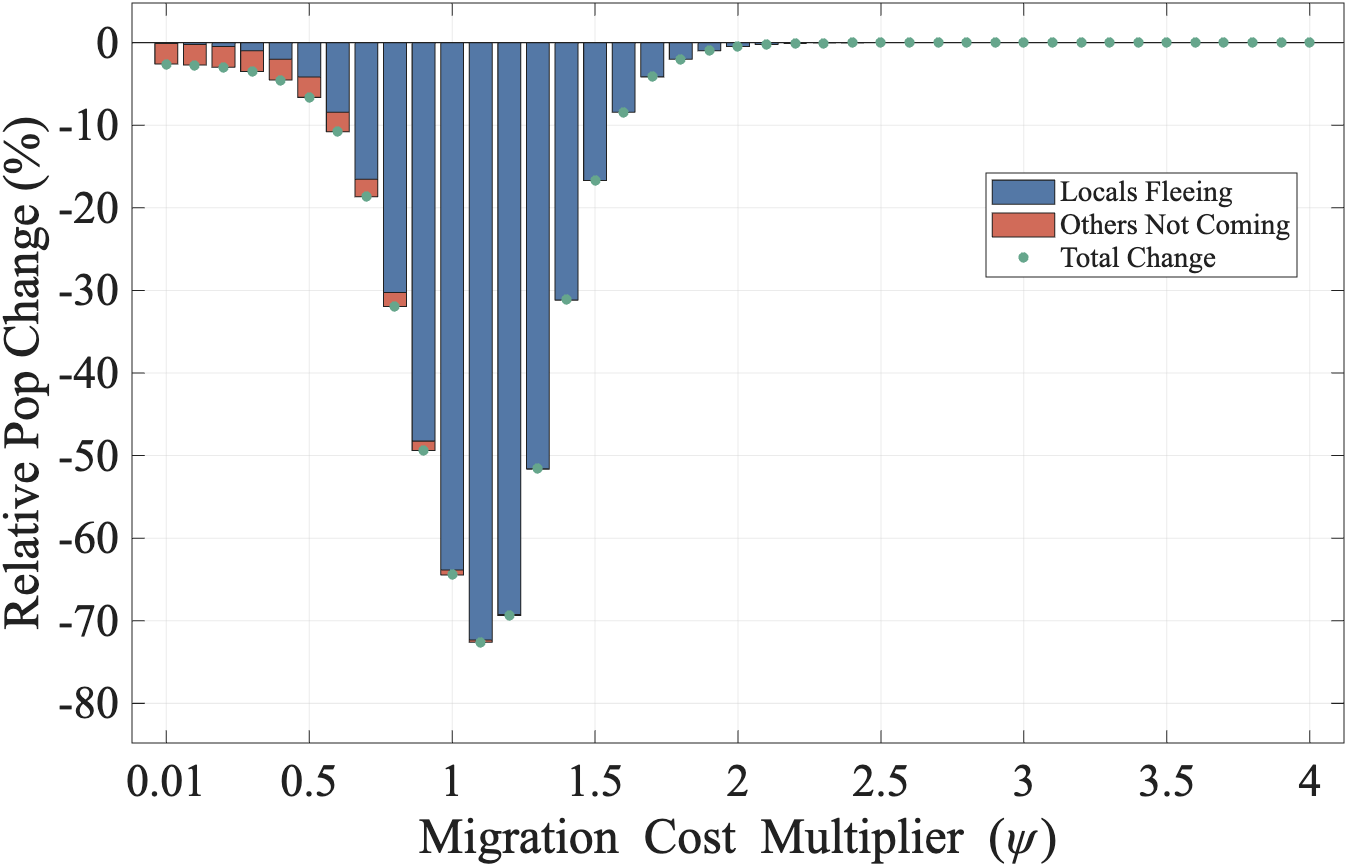
\includegraphics[width=\textwidth, height=0.40\textheight, keepaspectratio]{../Output/big_nu/graph_ushape/ushape_t500_florida.png}\\
            \vspace{0.02cm}
            \begin{tcolorbox}[leafbox]
                \tiny \textbf{Damaged State:} At low $\psi$, locals leave rapidly. At high $\psi$, locals are trapped, but outside inflows collapse, creating long-run population decline.
            \end{tcolorbox}
        \end{column}
        \begin{column}{0.485\textwidth}
            \centering
            \textbf{\scriptsize (b) Washington: Inflow Surge vs. Mobility Barrier}\\
            \vspace{0.02cm}
            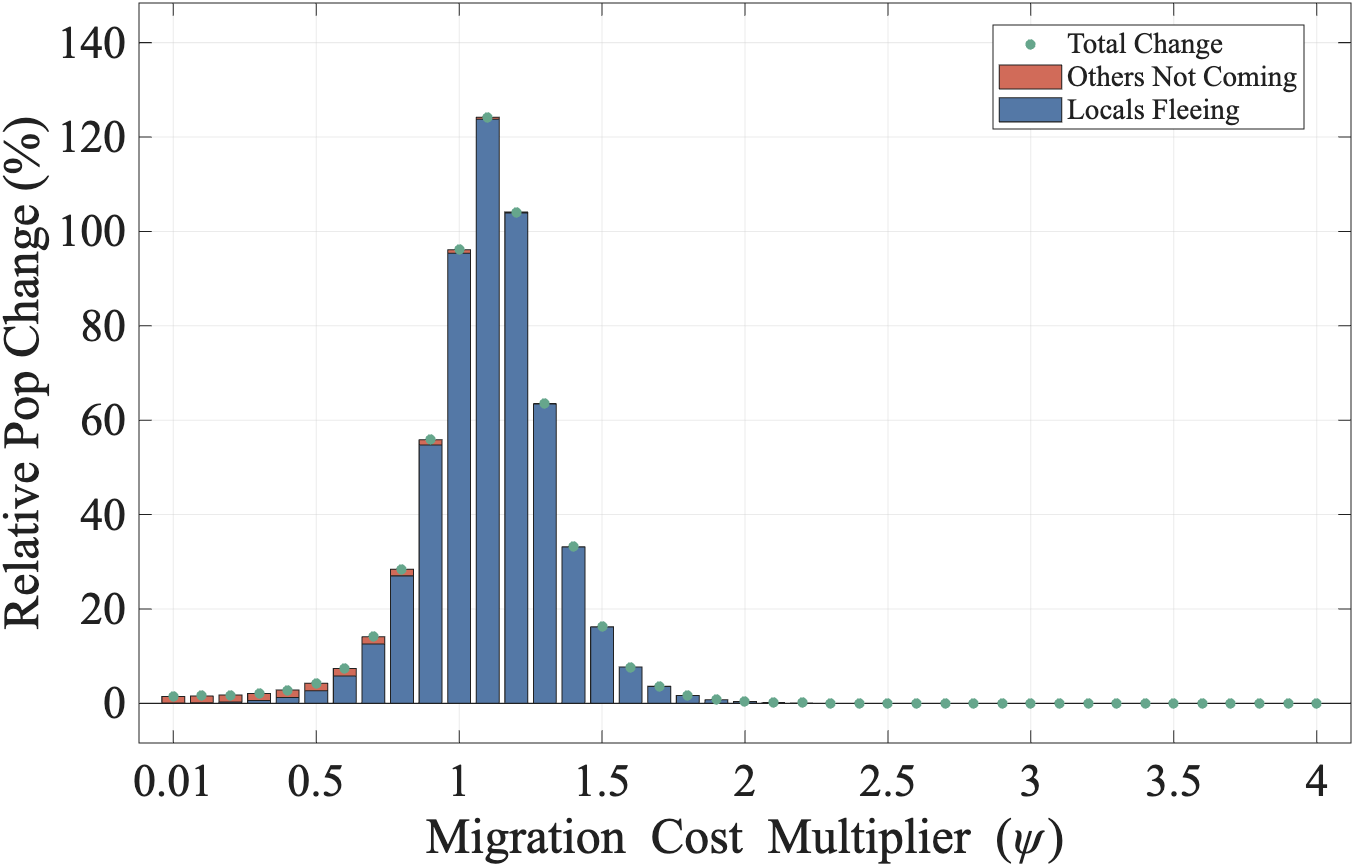
\includegraphics[width=\textwidth, height=0.40\textheight, keepaspectratio]{../Output/big_nu/graph_ushape/ushape_t500_washington.png}\\
            \vspace{0.02cm}
            \begin{tcolorbox}[leafbox]
                \tiny \textbf{Haven State:} Inflow surges when migration frictions are low, but higher frictions restrict haven access, dampening net population gains.
            \end{tcolorbox}
        \end{column}
    \end{columns}
\end{frame}

% R2 SLIDE 3: MECHANISM OF MYOPIA
\begin{frame}{Appendix: Mechanism of Myopia --- The Wealth Collapse \hfill \hyperlink{main:myopia}{\scriptsize\beamerreturnbutton{Return}}}\label{backup:myopia_dynamics}
    \begin{columns}[T]
        \begin{column}{0.485\textwidth}
            \centering
            \textbf{\scriptsize (a) National Wealth Trajectory under Myopia}\\
            \vspace{0.02cm}
            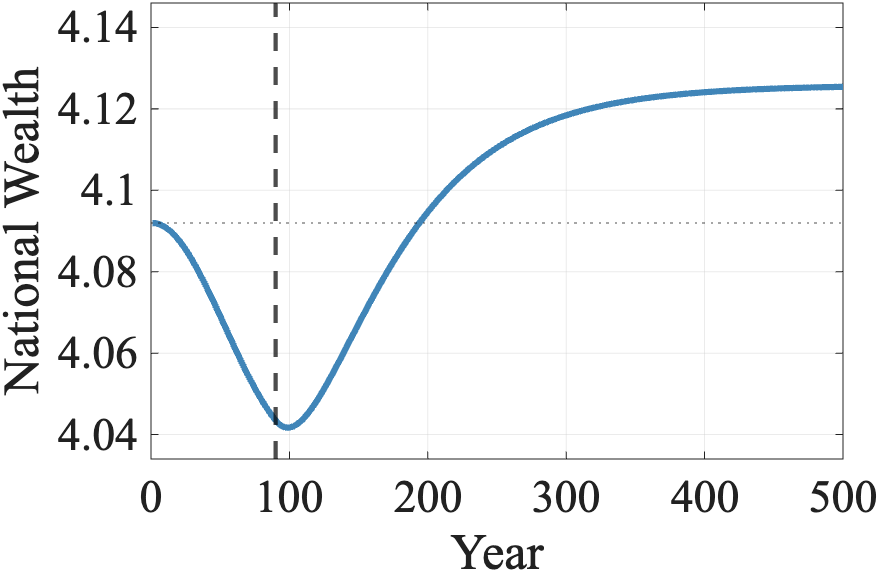
\includegraphics[width=\textwidth, height=0.38\textheight, keepaspectratio]{../Output/big_nu/graph_myopia/dynamic_moments/dynamic_moments_national_wealth.png}\\
            \vspace{0.02cm}
            \begin{itemize}\scriptsize\setlength{\itemsep}{1pt}
                \item Wealth collapses as shocks hit unexpectedly without advance precautionary saving.
            \end{itemize}
        \end{column}
        \begin{column}{0.485\textwidth}
            \centering
            \textbf{\scriptsize (b) Wealth-to-Income Ratio ($(W/Y)_t$)}\\
            \vspace{0.02cm}
            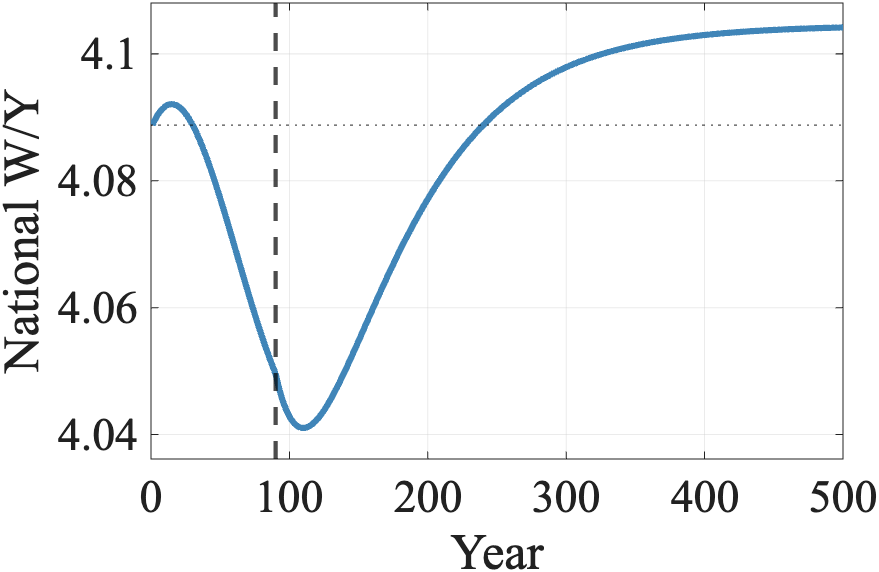
\includegraphics[width=\textwidth, height=0.38\textheight, keepaspectratio]{../Output/big_nu/graph_myopia/dynamic_moments/dynamic_moments_national_wy.png}\\
            \vspace{0.02cm}
            \begin{tcolorbox}[takeawaybox]
                \tiny \textbf{Welfare Penalty:} Myopic households suffer a $4\times$ larger welfare drop in 2100 ($-0.8\%$ vs $-0.2\%$) and take 400 years to reach steady state.
            \end{tcolorbox}
        \end{column}
    \end{columns}
\end{frame}

% R2 SLIDE 5: STRUCTURAL HAND-TO-MOUTH
\begin{frame}{Appendix: Hand-to-Mouth Adaptation --- Mobility without Savings \hfill \hyperlink{main:margins}{\scriptsize\beamerreturnbutton{Return}}}\label{backup:nosaving_struct}
    \begin{columns}[T]
        \begin{column}{0.485\textwidth}
            \centering
            \textbf{\scriptsize (a) Population Reallocation without Savings}\\
            \vspace{0.02cm}
            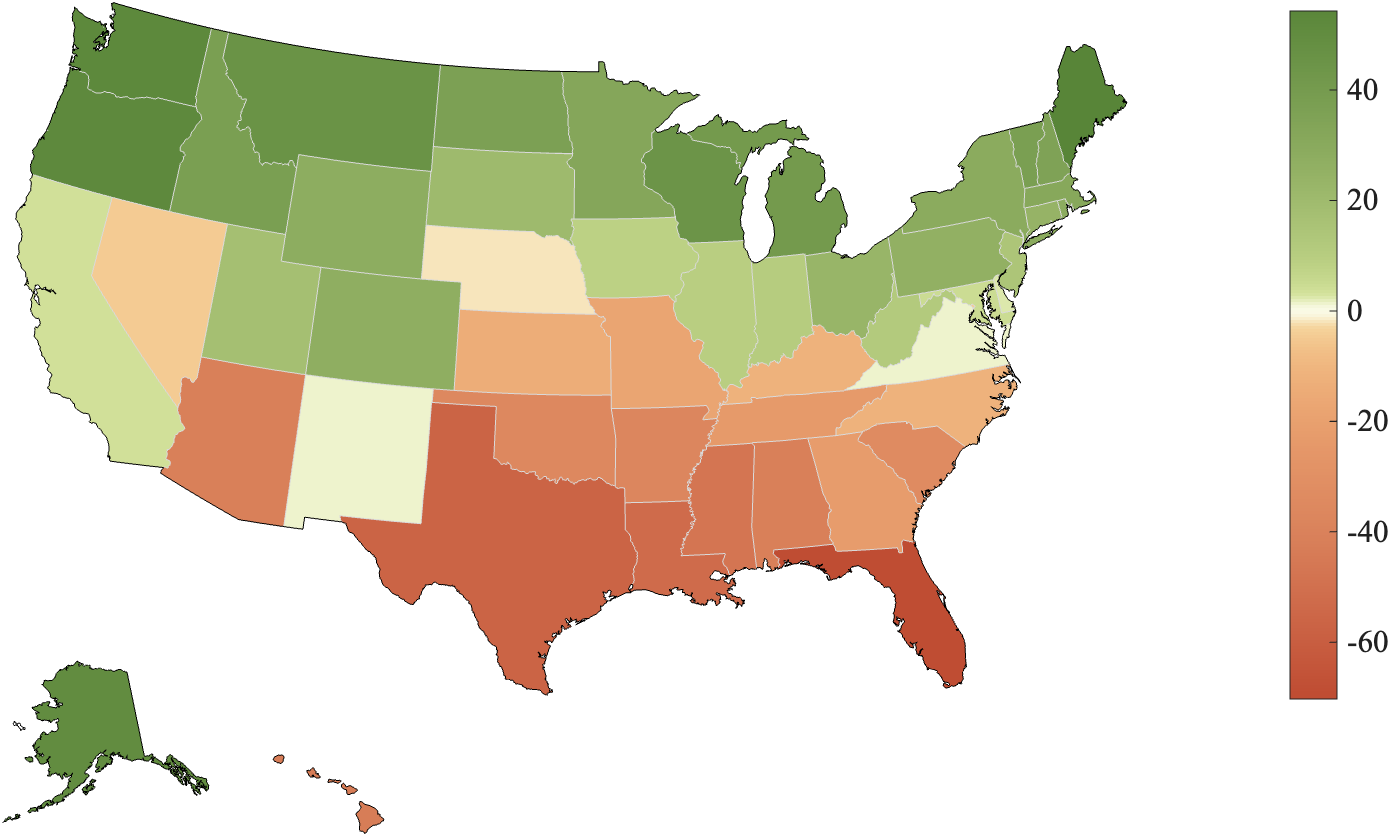
\includegraphics[width=\textwidth, height=0.38\textheight, keepaspectratio]{../Output/big_nu/graph_no_saving_struct/transition_maps/transition_maps_local_pop_changes_pct.png}\\
            \vspace{0.02cm}
            \begin{itemize}\scriptsize\setlength{\itemsep}{1pt}
                \item Gross mobility rises ($2.50\% \to 2.75\%$) as workers flee damaged South.
            \end{itemize}
        \end{column}
        \begin{column}{0.485\textwidth}
            \centering
            \textbf{\scriptsize (b) Local Welfare Drop ($\Delta\text{CE}_\ell$ [\%])}\\
            \vspace{0.02cm}
            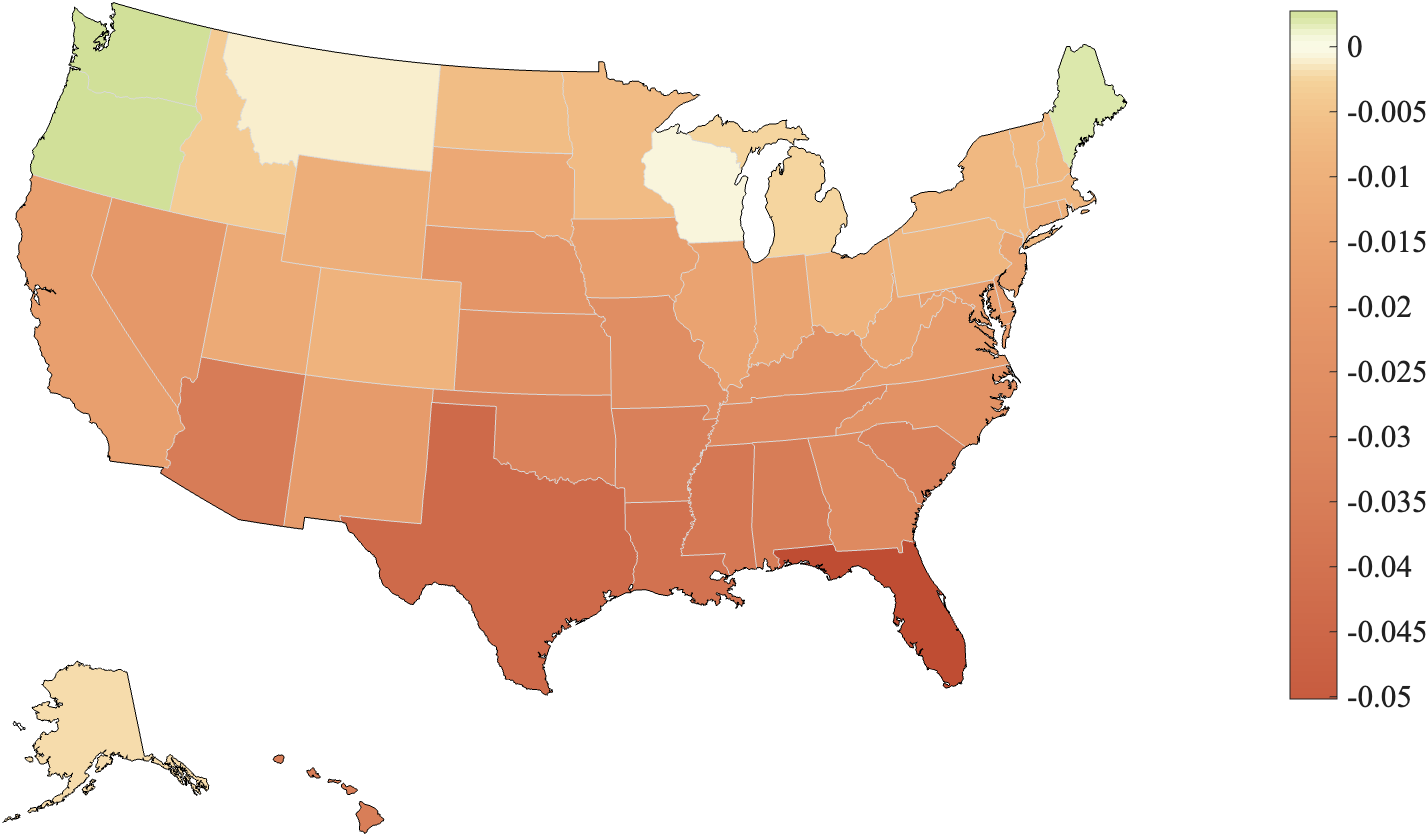
\includegraphics[width=\textwidth, height=0.38\textheight, keepaspectratio]{../Output/big_nu/graph_no_saving_struct/transition_maps/transition_maps_delta_mean_welfare_ce.png}\\
            \vspace{0.02cm}
            \begin{tcolorbox}[takeawaybox]
                \tiny \textbf{Variance Barrier:} High-wage Northern havens impose high uninsurable risk $\frac{1}{2}(\gamma\tilde{w}_\ell)^2\sigma_\eta^2$. Without savings, workers cannot buffer this risk $\to$ aggregate welfare loss reaches $-2.80\%$.
            \end{tcolorbox}
        \end{column}
    \end{columns}
\end{frame}

% R2 SLIDE 6: CLIMATE UNCERTAINTY & ENDOGENOUS VARIANCE SHOCKS
\begin{frame}{Appendix: Climate Volatility \& Precautionary Wealth Amplification \hfill \hyperlink{main:saving_risk}{\scriptsize\beamerreturnbutton{Return}}}\label{backup:uncertainty_var}
    \begin{columns}[T]
        \begin{column}{0.485\textwidth}
            \centering
            \textbf{\scriptsize (a) Spatial Variance Multiplier Map}\\
            \vspace{0.02cm}
            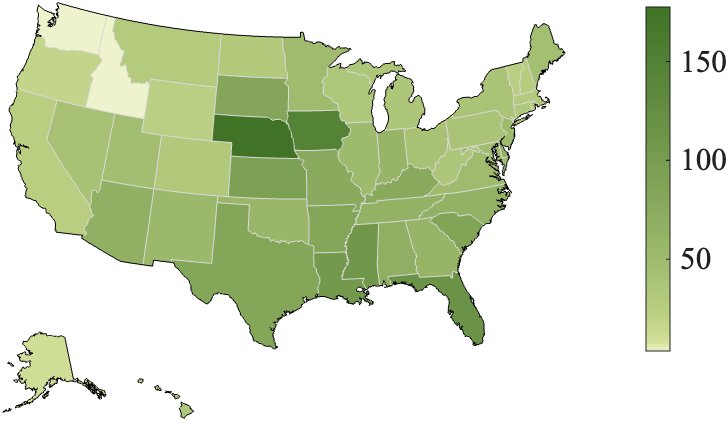
\includegraphics[width=\textwidth, height=0.38\textheight, keepaspectratio]{../Output/big_nu/graph_uncertainty_variance_shocks/variance_map.png}\\
            \vspace{0.02cm}
            \begin{itemize}\scriptsize\setlength{\itemsep}{1pt}
                \item Volatility scales with damage: $\sigma_{\eta,\ell,t}^2 = \bar{\sigma}_{\eta,\ell}^2 \left(1 + 50 |\Delta w_\ell| \frac{t}{T}\right)$.
            \end{itemize}
        \end{column}
        \begin{column}{0.485\textwidth}
            \centering
            \textbf{\scriptsize (b) Precautionary Wealth Surge}\\
            \vspace{0.02cm}
            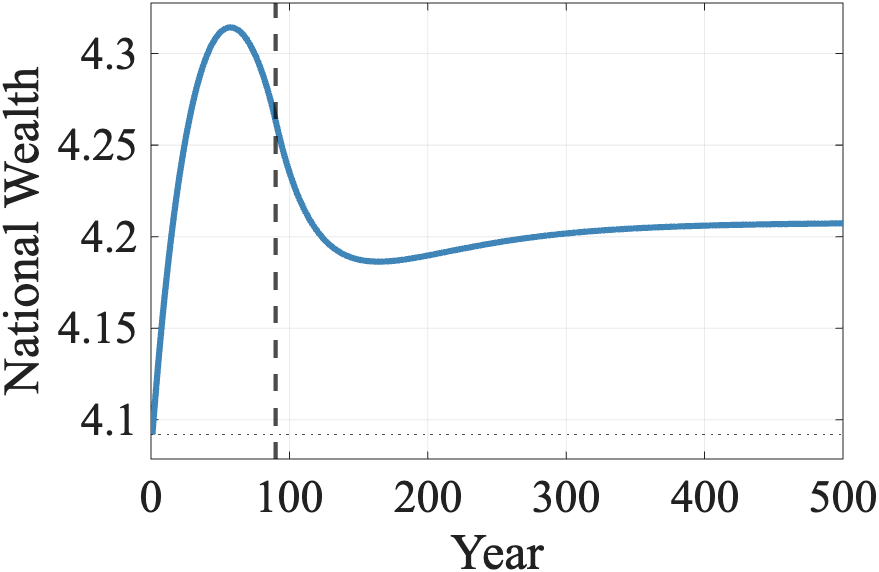
\includegraphics[width=\textwidth, height=0.38\textheight, keepaspectratio]{../Output/big_nu/graph_uncertainty_variance_shocks/dynamic_moments/dynamic_moments_national_wealth.png}\\
            \vspace{0.02cm}
            \begin{tcolorbox}[takeawaybox]
                \tiny \textbf{Precautionary Surge:} Endogenous climate volatility amplifies precautionary savings accumulation from $+4.5\%$ to \textbf{$+8.2\%$}, showing the heightened value of liquid self-insurance.
            \end{tcolorbox}
        \end{column}
    \end{columns}
\end{frame}

% R2 SLIDE 7: ROBUSTNESS TO MIGRATION ELASTICITY
\begin{frame}{Appendix: Robustness to Migration Elasticity ($\nu = 2.16$ vs $\nu = 4.0$) \hfill \hyperlink{main:calibration}{\scriptsize\beamerreturnbutton{Return}}}\label{backup:small_nu_robustness}
    \begin{columns}[T]
        \begin{column}{0.485\textwidth}
            \centering
            \textbf{\scriptsize (a) Precautionary Wealth Peak ($\nu = 2.16$)}\\
            \vspace{0.02cm}
            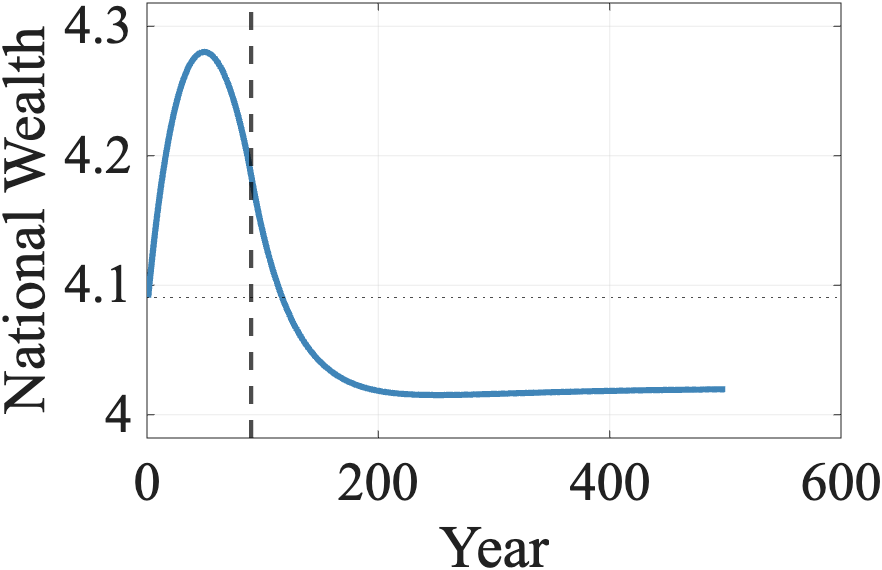
\includegraphics[width=\textwidth, height=0.38\textheight, keepaspectratio]{../Output/small_nu/graph_perfect_foresight/dynamic_moments/dynamic_moments_national_wealth.png}\\
            \vspace{0.02cm}
            \begin{itemize}\scriptsize\setlength{\itemsep}{1pt}
                \item Precautionary peak is robust: $+4.2\%$ vs $+4.5\%$.
            \end{itemize}
        \end{column}
        \begin{column}{0.485\textwidth}
            \centering
            \textbf{\scriptsize (b) Spatial Sorting against Dvorkin Target}\\
            \vspace{0.02cm}
            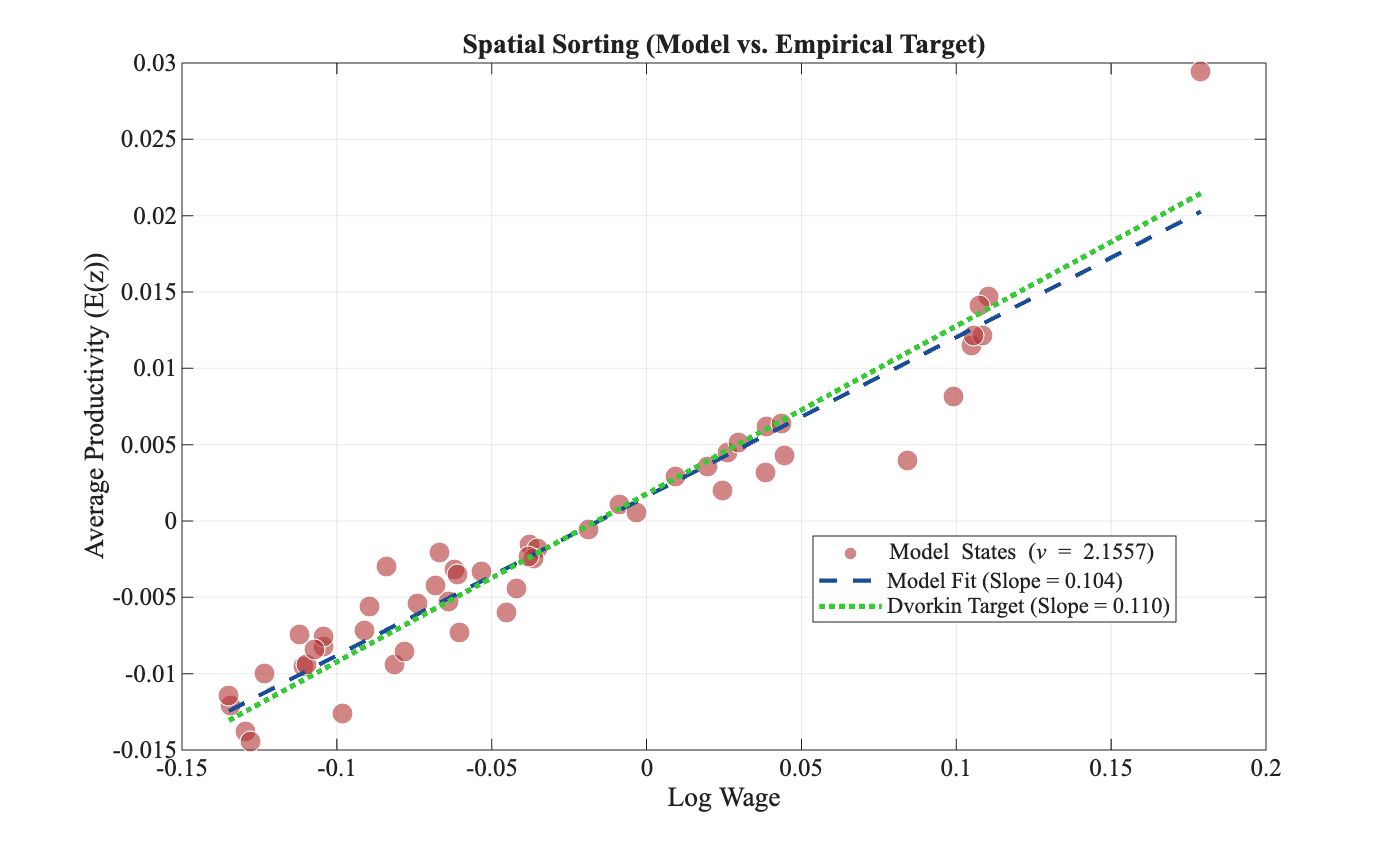
\includegraphics[width=\textwidth, height=0.38\textheight, keepaspectratio]{../Output/small_nu/graph_spatial_sorting/spatial_sorting.png}\\
            \vspace{0.02cm}
            \begin{tcolorbox}[takeawaybox]
                \tiny \textbf{Sorting Match:} $\nu = 2.16$ matches the empirical sorting slope of $E(z)$ on $\log(w)$ (0.110 target from Dvorkin \& Greaney 2025), confirming core model mechanics.
            \end{tcolorbox}
        \end{column}
    \end{columns}
\end{frame}

% R2 SLIDE 8: OUT-OF-SAMPLE EMPIRICAL FIT
\begin{frame}{Appendix: Out-of-Sample Empirical Fit (Geowealth-US \& ACS Migration) \hfill \hyperlink{main:calibration}{\scriptsize\beamerreturnbutton{Return}}}\label{backup:out_sample_fit}
    \begin{columns}[T]
        \begin{column}{0.485\textwidth}
            \centering
            \textbf{\scriptsize (a) State Mean Wealth (Model vs Geowealth-US)}\\
            \vspace{0.02cm}
            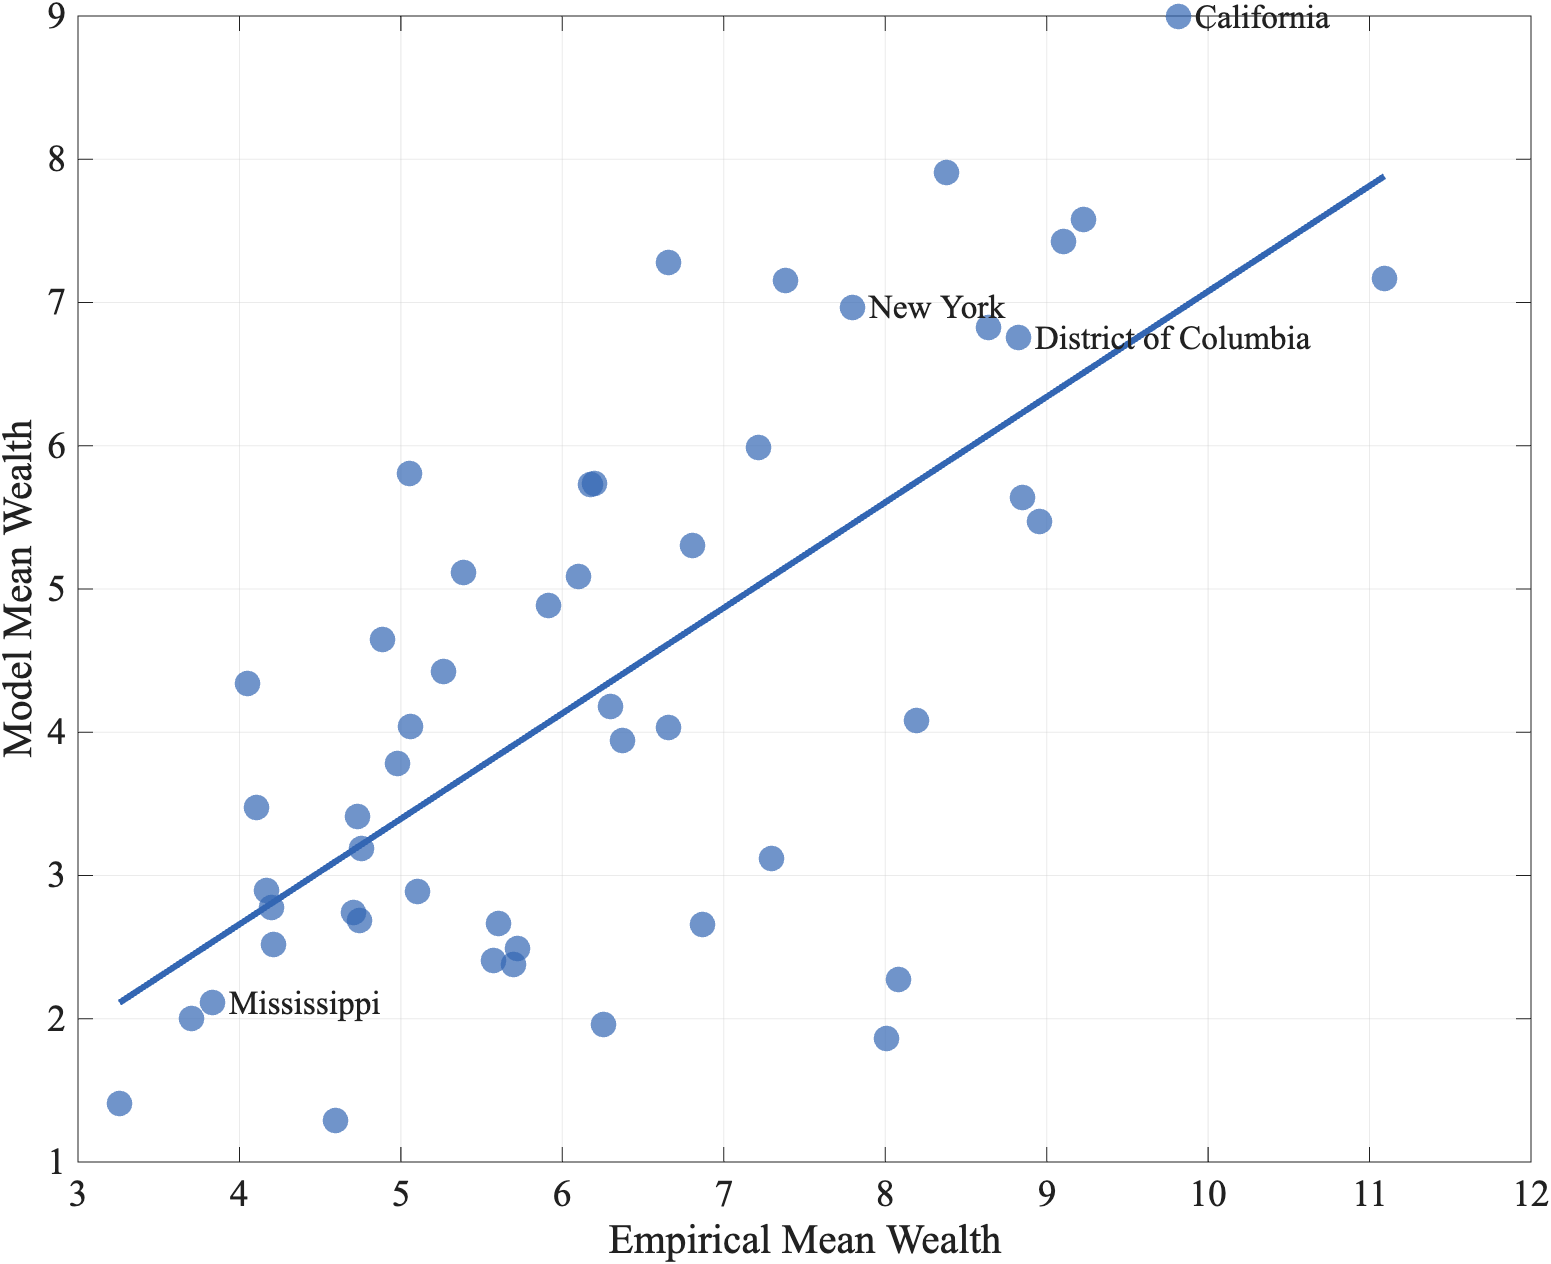
\includegraphics[width=\textwidth, height=0.38\textheight, keepaspectratio]{../Output/graph_comparison/out_sample_fit/out_sample_fit_model_mean_wealth.png}\\
            \vspace{0.02cm}
            \begin{itemize}\scriptsize\setlength{\itemsep}{1pt}
                \item Strong cross-state wealth correlation ($R^2 = 0.46, r = 0.68$).
            \end{itemize}
        \end{column}
        \begin{column}{0.485\textwidth}
            \centering
            \textbf{\scriptsize (b) Bilateral Migration Matrix Fit (Model vs ACS)}\\
            \vspace{0.02cm}
            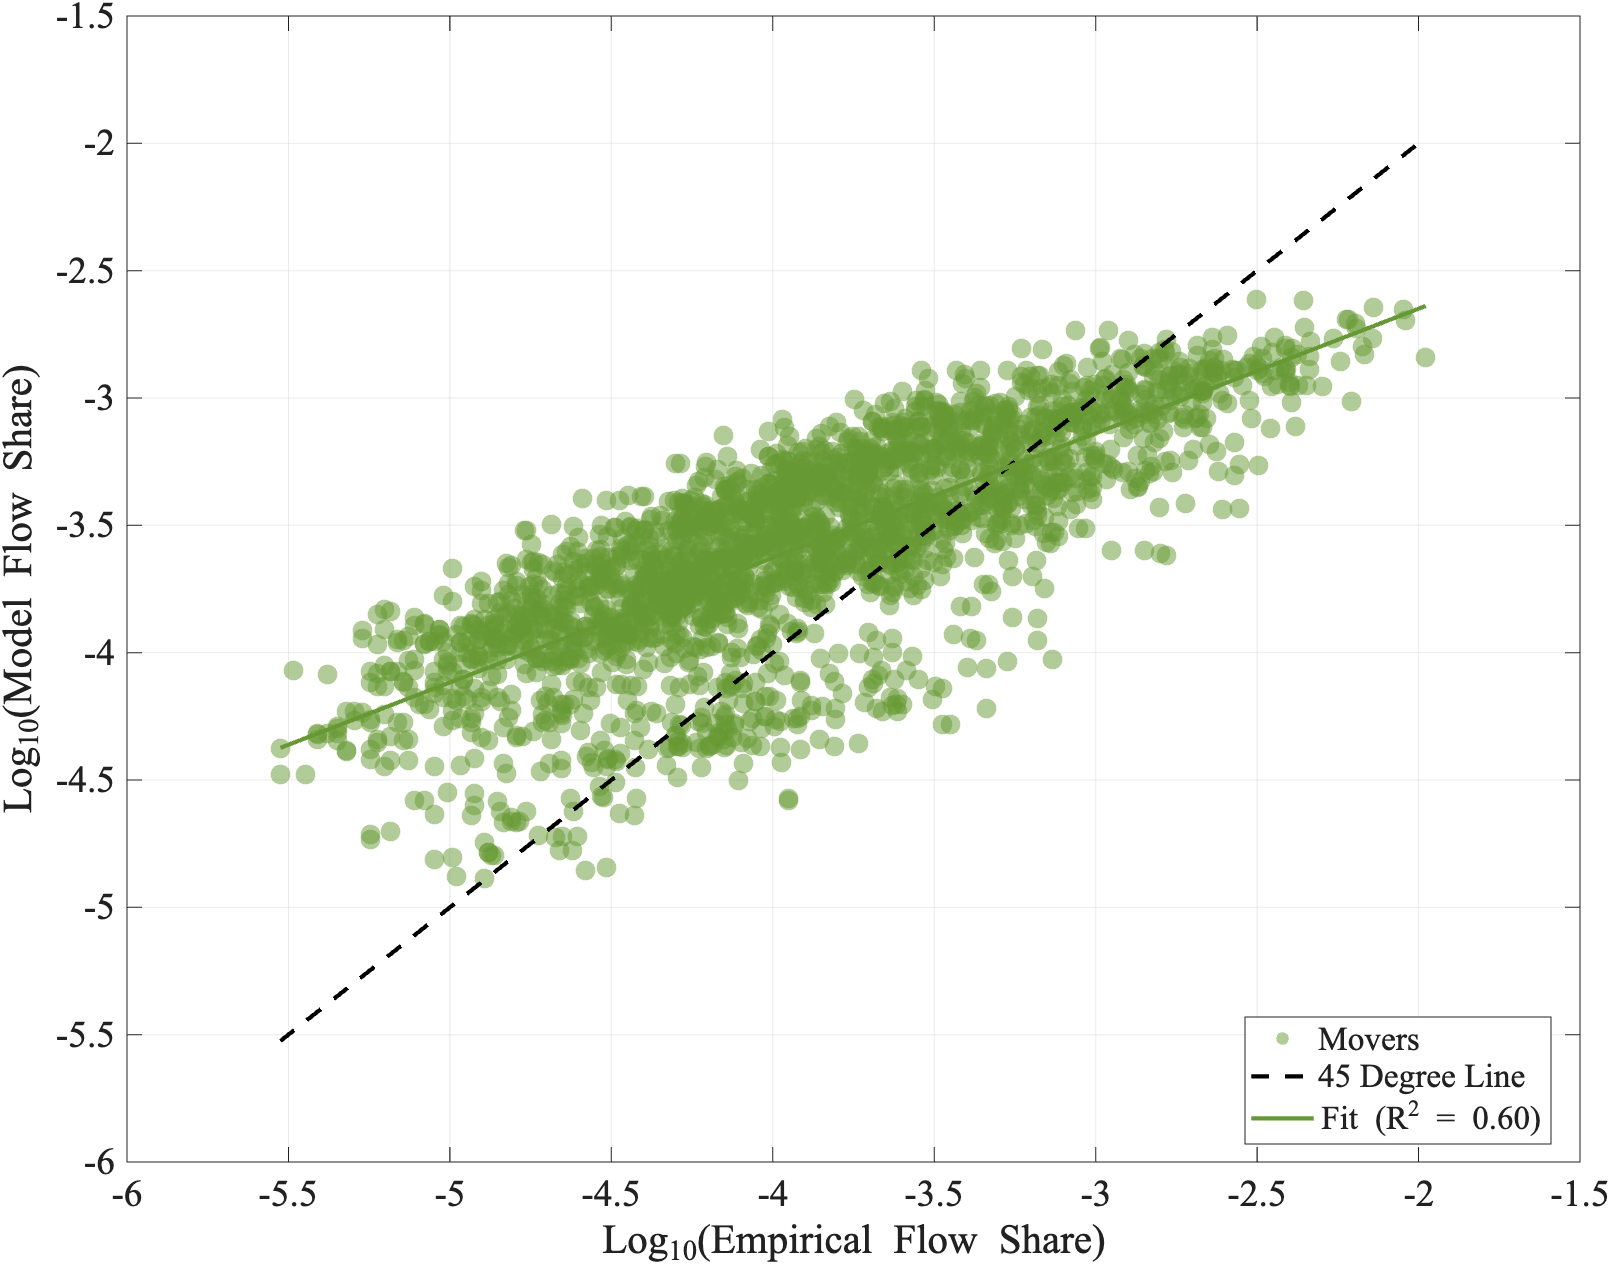
\includegraphics[width=\textwidth, height=0.38\textheight, keepaspectratio]{../Output/graph_comparison/out_sample_fit/out_sample_fit_log_10_model_flow_share.png}\\
            \vspace{0.02cm}
            \begin{tcolorbox}[takeawaybox]
                \tiny \textbf{Empirical Fit:} Log bilateral migration shares align tightly along the 45-degree line with ACS 2010--2019 inter-state mobility ($R^2 = 0.52, r = 0.72$).
            \end{tcolorbox}
        \end{column}
    \end{columns}
\end{frame}

% R2 SLIDE 9: DYNAMIC SPATIAL INEQUALITY
\begin{frame}{Appendix: Dynamic Spatial Inequality Across US States \hfill \hyperlink{main:spatial_hetero}{\scriptsize\beamerreturnbutton{Return}}}\label{backup:inequality_dynamics}
    \begin{columns}[T]
        \begin{column}{0.485\textwidth}
            \centering
            \textbf{\scriptsize (a) National Between-State Welfare Inequality}\\
            \vspace{0.02cm}
            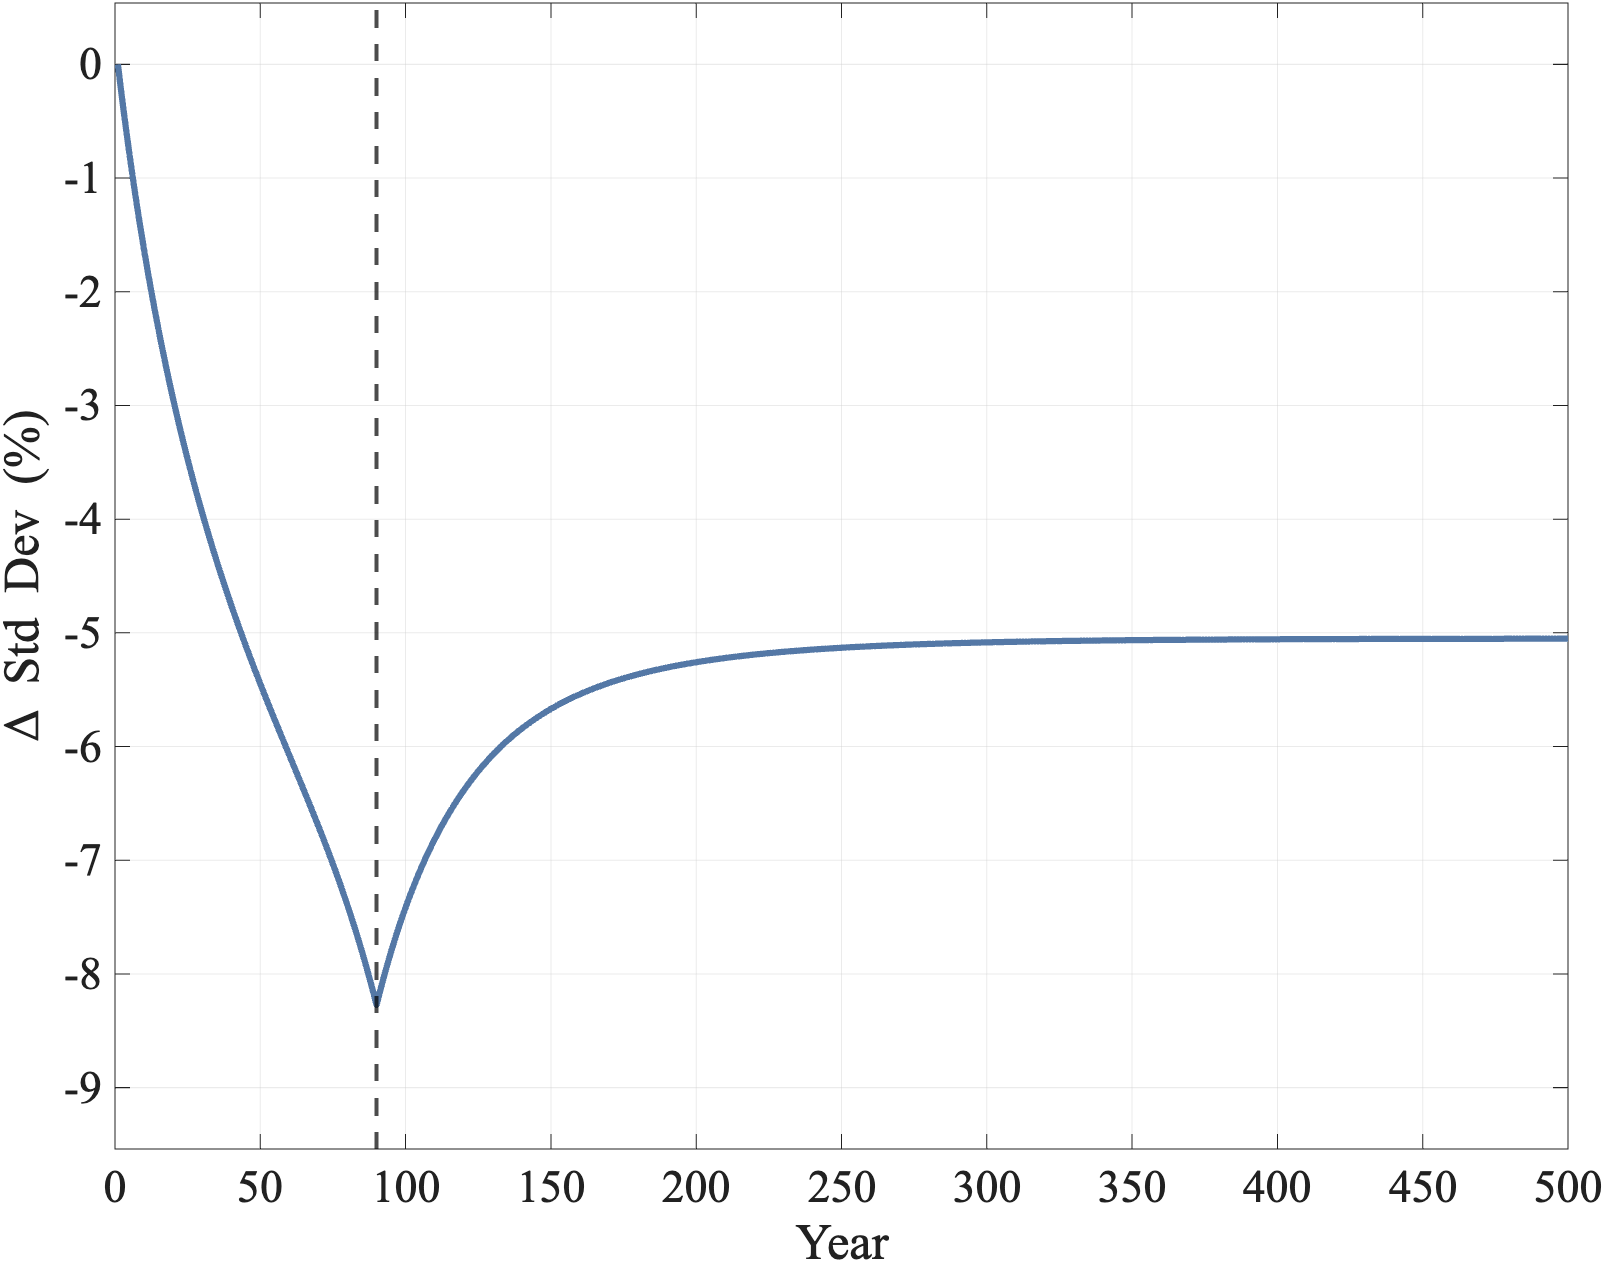
\includegraphics[width=\textwidth, height=0.38\textheight, keepaspectratio]{../Output/big_nu/graph_perfect_foresight/welfare_transition/welfare_transition_welfare_inequality.png}\\
            \vspace{0.02cm}
            \begin{itemize}\scriptsize\setlength{\itemsep}{1pt}
                \item Spatial standard deviation of Certainty Equivalent rises $+18\%$.
            \end{itemize}
        \end{column}
        \begin{column}{0.485\textwidth}
            \centering
            \textbf{\scriptsize (b) Spatial Welfare Variance Map ($\Delta\text{Var}(\text{CE})_\ell$)}\\
            \vspace{0.02cm}
            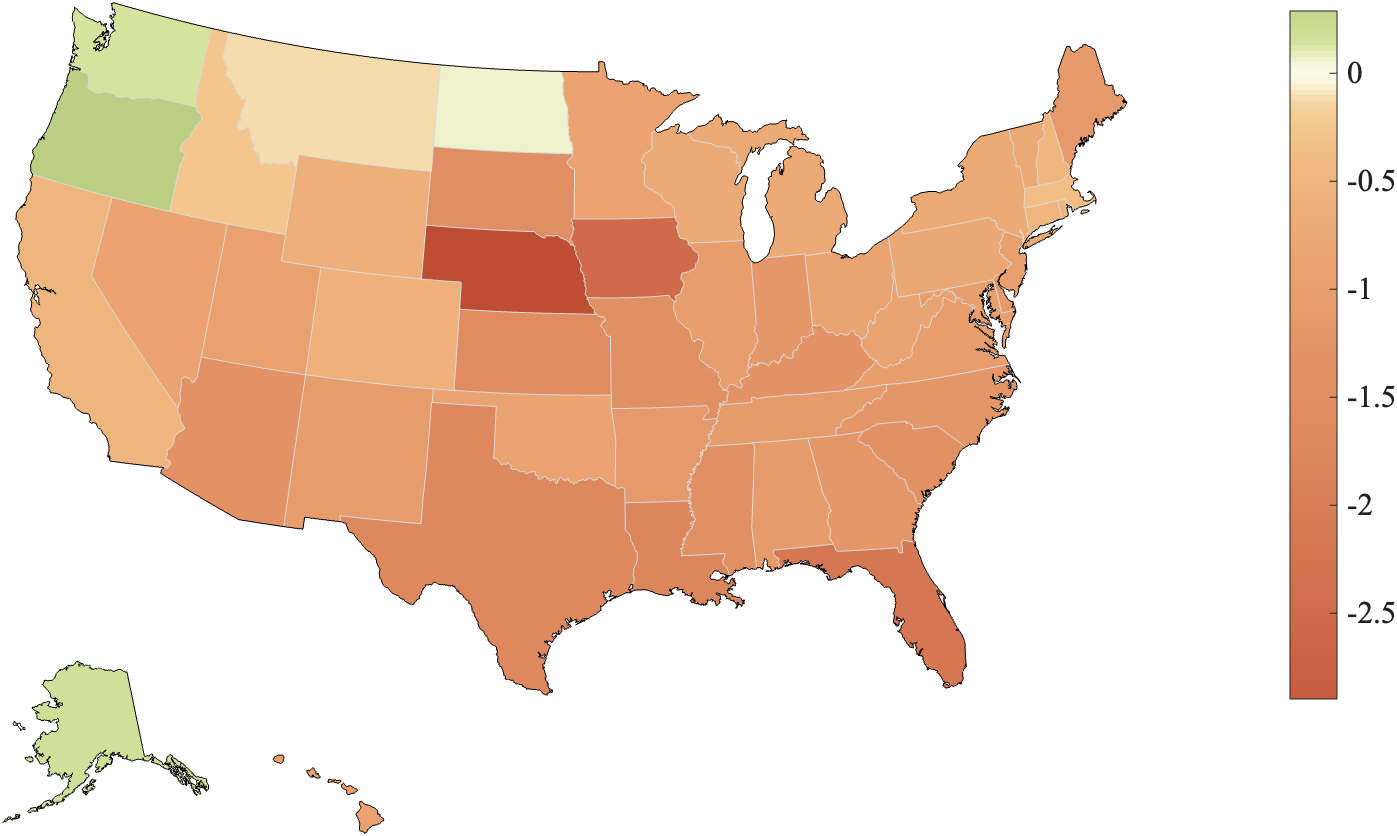
\includegraphics[width=\textwidth, height=0.38\textheight, keepaspectratio]{../Output/big_nu/graph_perfect_foresight/welfare_wealth_inequality_maps/welfare_wealth_inequality_maps_welfare_inequality.png}\\
            \vspace{0.02cm}
            \begin{tcolorbox}[takeawaybox]
                \tiny \textbf{Divergence:} Climate change significantly widens regional living standard disparities, with within-state inequality expanding most in receiving Northern states.
            \end{tcolorbox}
        \end{column}
    \end{columns}
\end{frame}

% R2 SLIDE 10: XI PRODUCTIVITY GRADIENTS
\begin{frame}{Appendix: Continuation Value Field ($\Xi$) and Productivity Gradients \hfill \hyperlink{main:spatial_hetero}{\scriptsize\beamerreturnbutton{Return}}}\label{backup:xi_mechanics}
    \begin{columns}[T]
        \begin{column}{0.485\textwidth}
            \centering
            \textbf{\scriptsize (a) Policy Gradient $\Xi(z)$ across Productivity Grid}\\
            \vspace{0.02cm}
            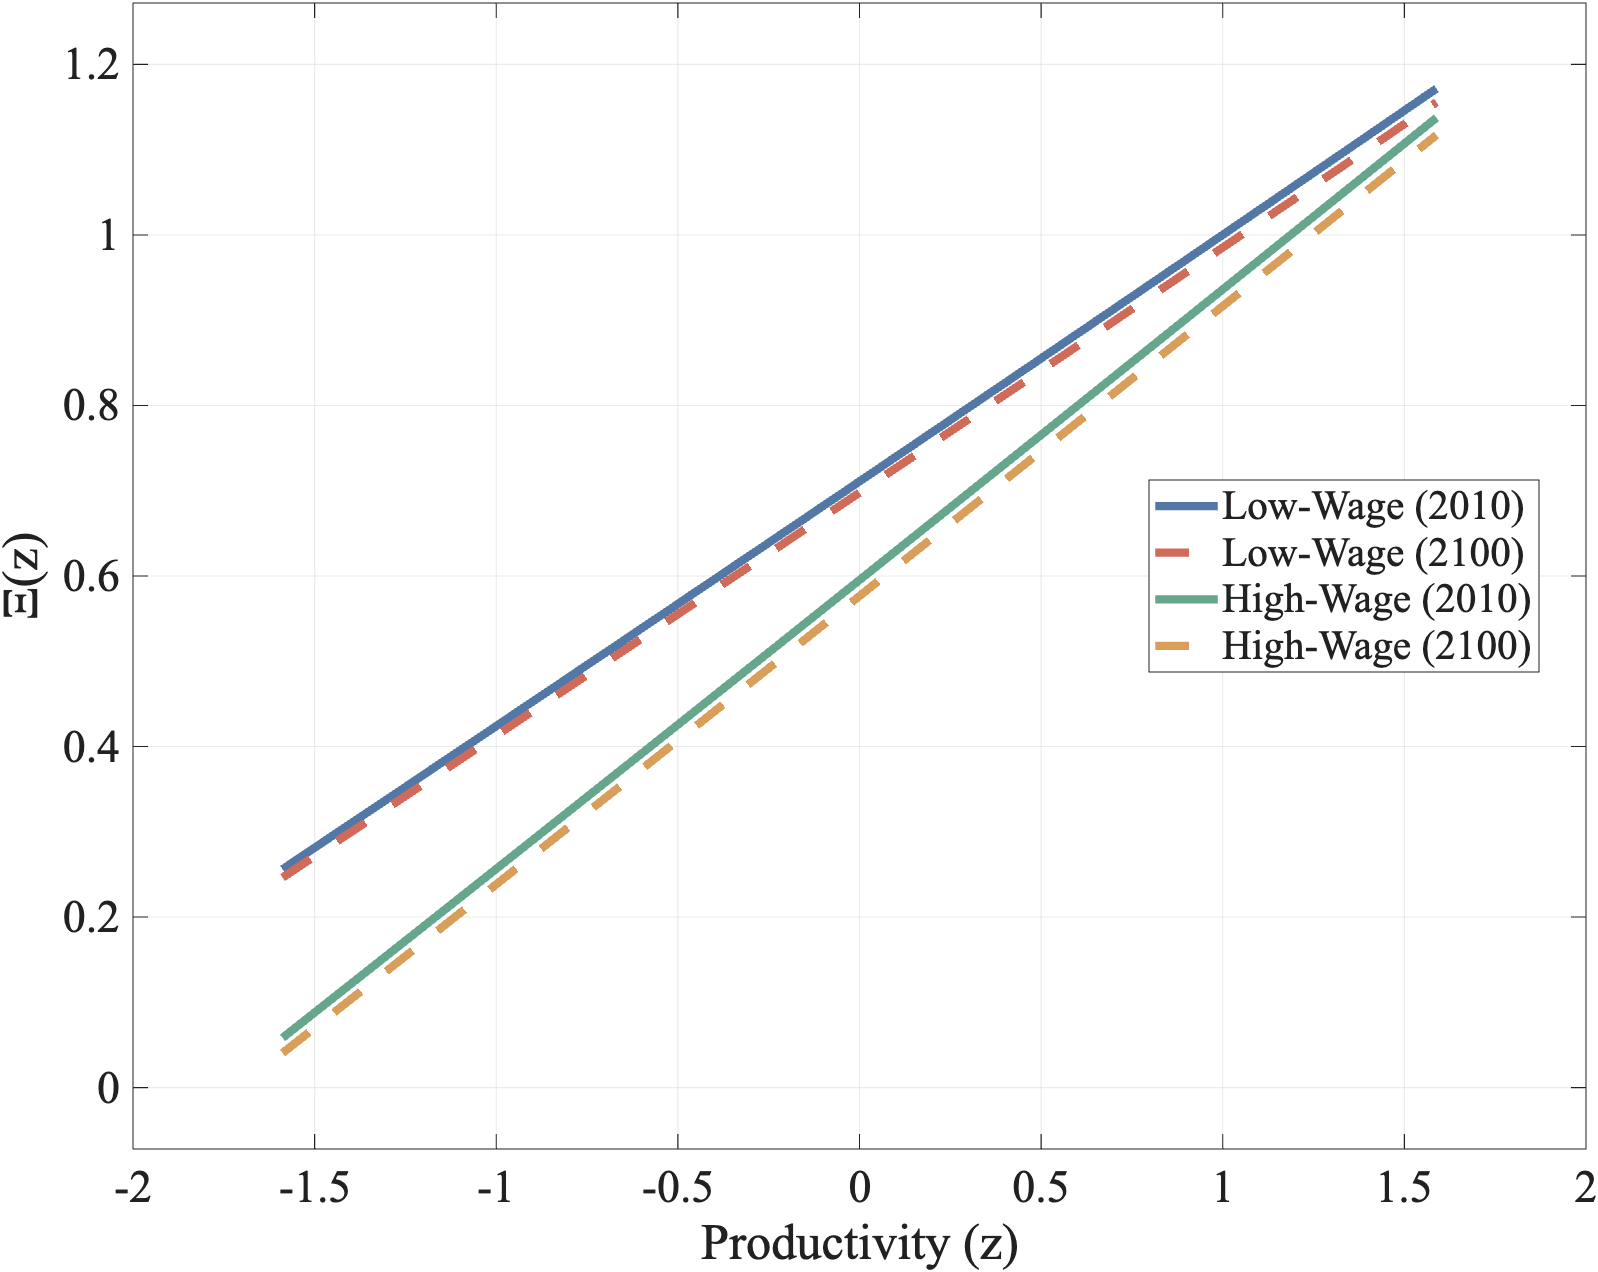
\includegraphics[width=\textwidth, height=0.38\textheight, keepaspectratio]{../Output/big_nu/graph_perfect_foresight/xi_transition/xi_transition_gradient_productivity.png}\\
            \vspace{0.02cm}
        \end{column}
        \begin{column}{0.485\textwidth}
            \centering
            \textbf{\scriptsize (b) Evolution of $\Xi_t(z=0)$ Across State Groups}\\
            \vspace{0.02cm}
            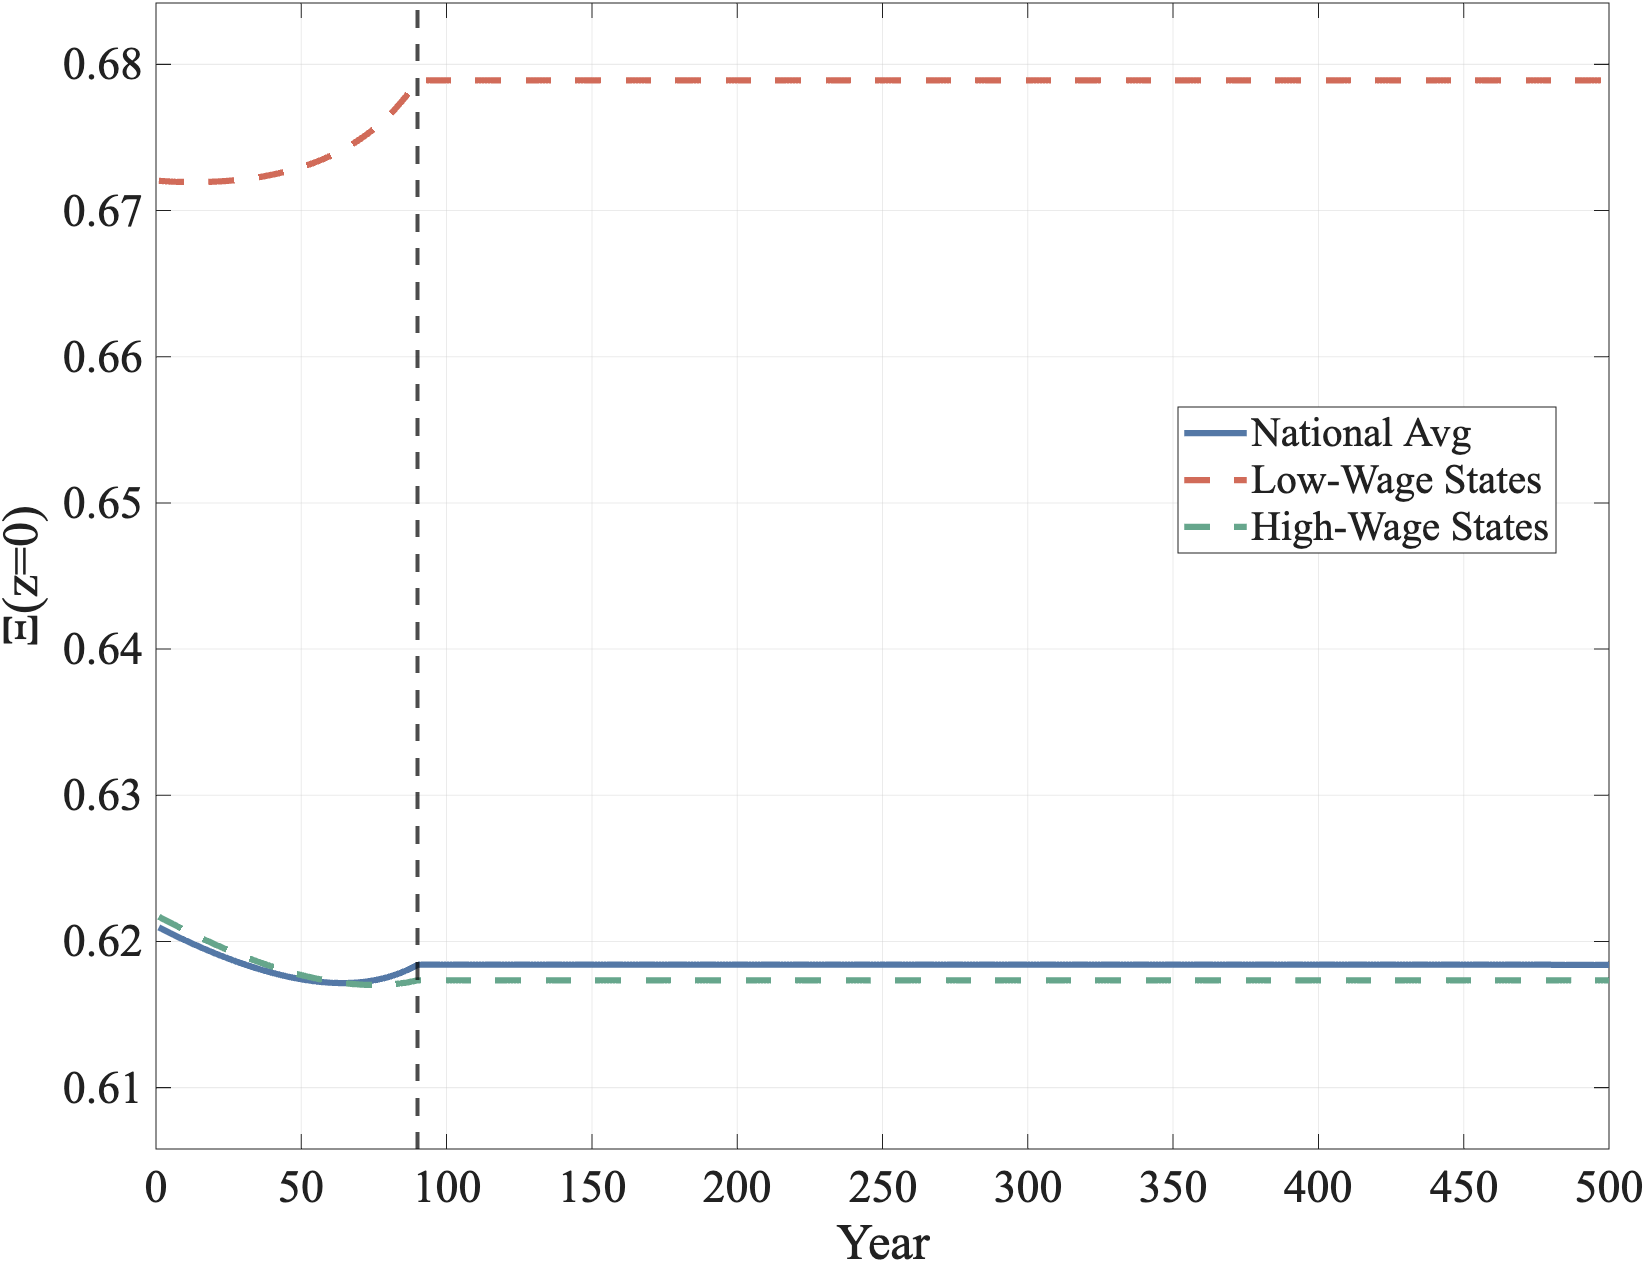
\includegraphics[width=\textwidth, height=0.38\textheight, keepaspectratio]{../Output/big_nu/graph_perfect_foresight/xi_transition/xi_transition_average_evolution.png}\\
            \vspace{0.02cm}
            \begin{tcolorbox}[takeawaybox]
                \tiny \textbf{Divergence in $\Xi$:} Continuation values in high-wage havens remain resilient, while low-wage and Southern states suffer sustained declines in their baseline consumption intercepts.
            \end{tcolorbox}
        \end{column}
    \end{columns}
\end{frame}

% R2 SLIDE 12: PRECAUTIONARY SAVING PEAK GEOGRAPHY
\begin{frame}{Appendix: Precautionary Saving Peak Geography ($t = 45$) \hfill \hyperlink{main:agg_dynamics}{\scriptsize\beamerreturnbutton{Return}}}\label{backup:peak_maps}
            \centering
            \textbf{\scriptsize (a) Wealth Accumulation at Peak ($t=45$)}\\
            \vspace{0.02cm}
            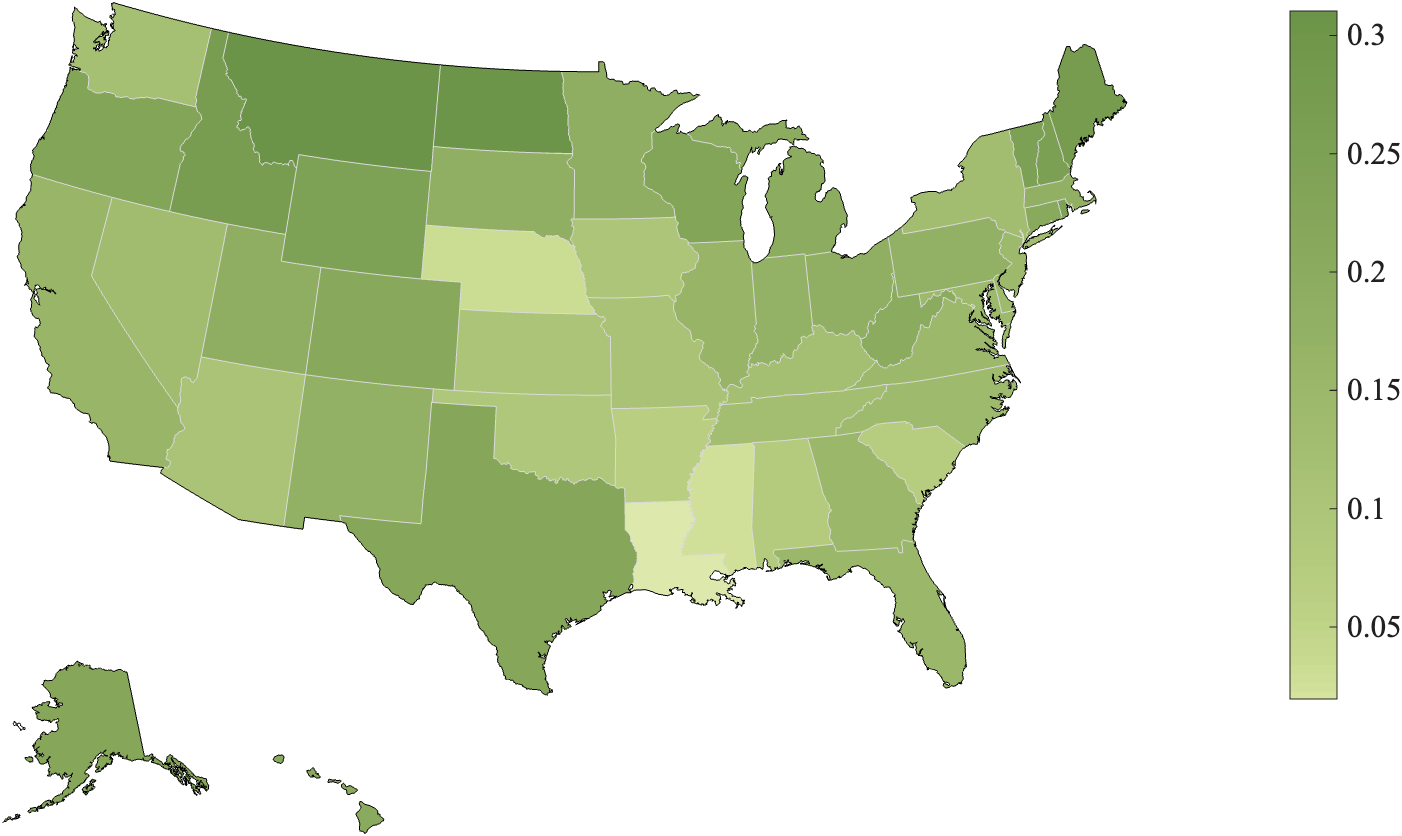
\includegraphics[width=\textwidth, height=0.38\textheight, keepaspectratio]{../Output/big_nu/graph_perfect_foresight/peak_transition_maps/peak_transition_maps_wealth_accumulation_peak.png}\\
            \vspace{0.02cm}
            \begin{itemize}\scriptsize\setlength{\itemsep}{1pt}
                \item Southern coastal states accumulate largest emergency wealth.
            \end{itemize}
\end{frame}

% ADDITIONAL POLICY SCENARIO: HIGH MOBILITY
\begin{frame}{Appendix: Policy Counterfactual: High Migration Mobility ($0.9\times\psi$) \hfill \hyperlink{main:margins}{\scriptsize\beamerreturnbutton{Return}}}\label{backup:big_migration_did}
    \begin{columns}[onlytextwidth, T]
        \begin{column}{0.485\textwidth}
            \centering
            \textbf{\scriptsize Population Changes ($\Delta\text{Pop}_\ell$ [pp])}\\
            \vspace{0.02cm}
            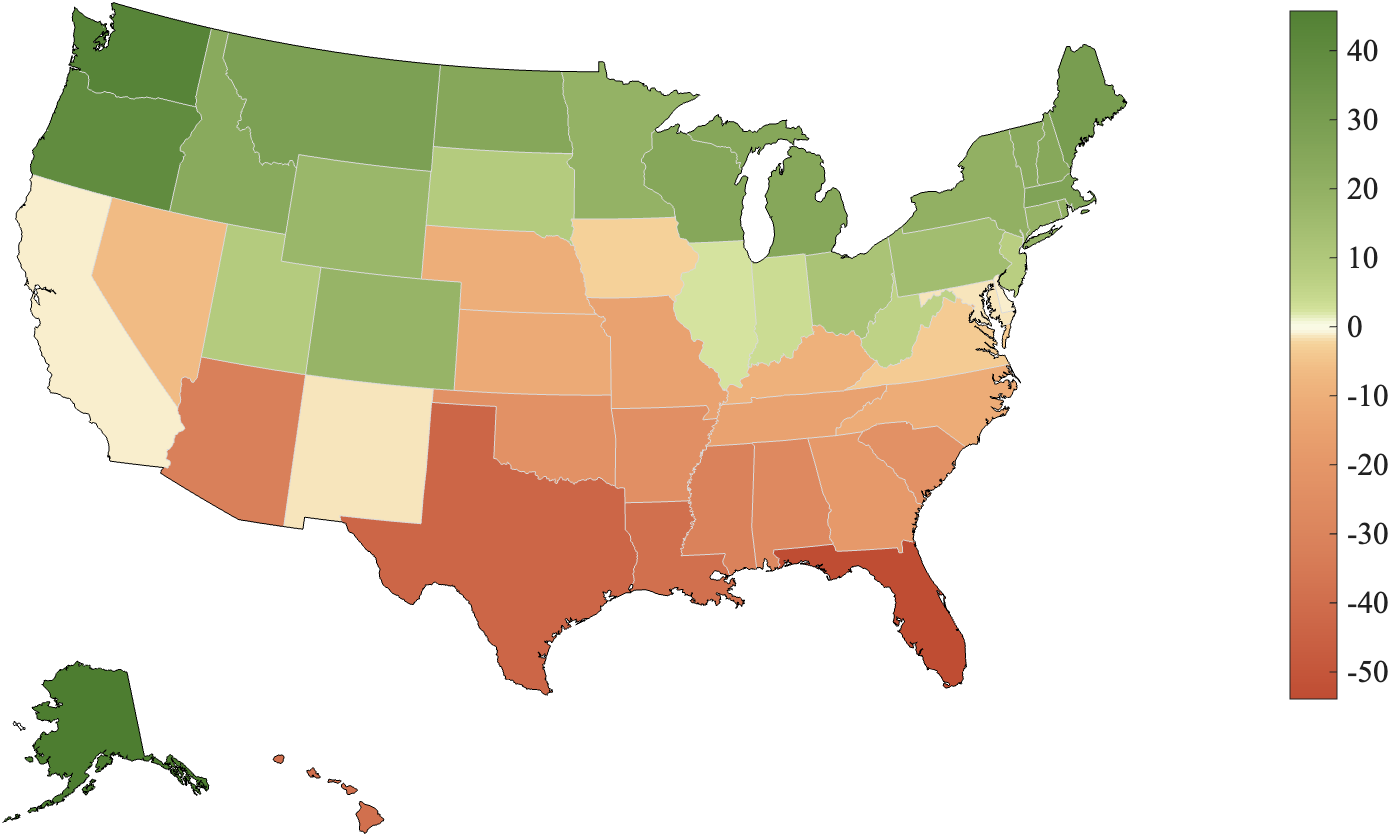
\includegraphics[width=\textwidth, height=0.38\textheight, keepaspectratio]{../Output/big_nu/graph_big_migration_did/transition_maps/transition_maps_local_pop_changes_pct.png}\\
            \vspace{0.02cm}
            \begin{itemize}\scriptsize\setlength{\itemsep}{1pt}
                \item Lower moving frictions reduceout-migration from vulnerable regions. (Weird Explanation)
            \end{itemize}
        \end{column}
        \begin{column}{0.485\textwidth}
            \centering
            \textbf{\scriptsize Wealth/Income Changes ($\Delta (W/Y)_\ell$)}\\
            \vspace{0.02cm}
            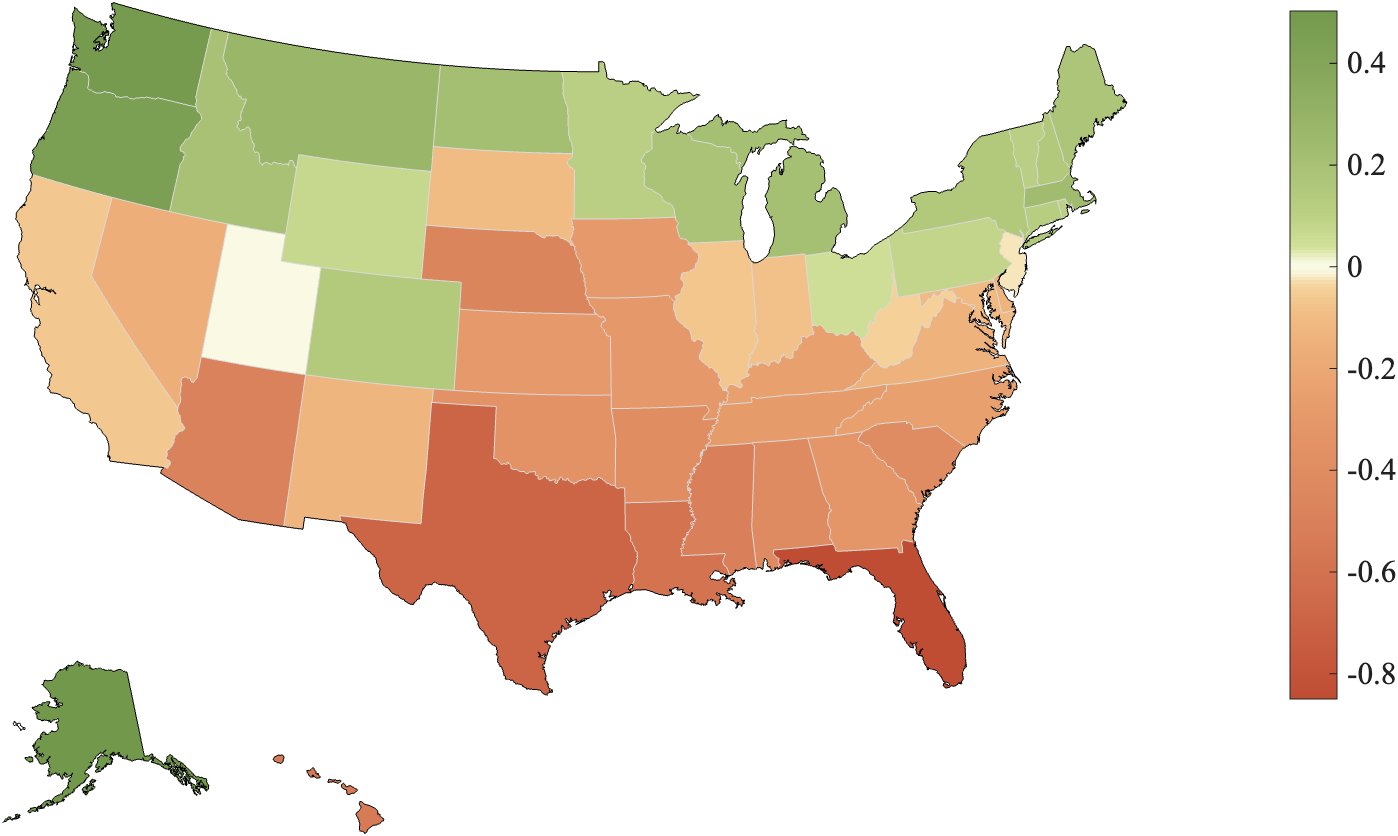
\includegraphics[width=\textwidth, height=0.38\textheight, keepaspectratio]{../Output/big_nu/graph_big_migration_did/transition_maps/transition_maps_wealth_income_ratio_changes.png}\\
            \vspace{0.02cm}
        \end{column}
    \end{columns}
\end{frame}

\end{document}


